\documentclass[aspectratio=169]{beamer}

\usepackage[T5]{fontenc}
\usepackage[utf8]{inputenc}
\usepackage{lmodern}

\usetheme{Madrid}

\usepackage{graphicx}
\usepackage{multicol}
\usepackage{amsmath,amssymb}

% Outline look: blue text, numbered, no balls
\setbeamertemplate{section in toc}{%
  \leavevmode\inserttocsectionnumber.~\inserttocsection\par}
\setbeamercolor{section in toc}{fg=blue}

\hypersetup{colorlinks=true, urlcolor=blue}

\newcommand{\backbtn}{%
  \hfill\hyperlink{outline}{\beamerbutton{Mục lục}}}


% Giảm khoảng cách trên/dưới công thức hiển thị để slide gọn hơn
\makeatletter
\def\tight@disp{\setlength\abovedisplayskip{4pt plus 2pt}%
  \setlength\belowdisplayskip{4pt plus 2pt}%
  \setlength\abovedisplayshortskip{2pt plus 1pt}%
  \setlength\belowdisplayshortskip{2pt plus 1pt}}
\g@addto@macro\normalsize{\tight@disp}
\g@addto@macro\small{\tight@disp}
\g@addto@macro\footnotesize{\tight@disp}
\g@addto@macro\scriptsize{\tight@disp}
\makeatother

\title[Tải trọng dọc trục]{Ứng suất và biến dạng: Tải trọng dọc trục}
\author[© N. V. Sỹ]{Nguyễn Văn Sỹ}
\institute[TNUT]{%
  Bộ môn Hệ thống Công nghiệp \\
  Trường Đại học Kỹ thuật Công nghiệp \\
  \href{mailto:vansy@tnut.edu.vn}{vansy@tnut.edu.vn}}
\date[Cơ học vật liệu]{\large Cơ học vật liệu – Tải trọng dọc trục \\[0.5em] \footnotesize \copyright\ Nguyễn Văn Sỹ}

\begin{document}

\begin{frame}
  \titlepage
\end{frame}
%====================
\begin{frame}{Tài liệu tham khảo}
	\small
	F. P. Beer, E. R. Johnston, Jr., J. T. DeWolf, D. F. Mazurek,
	\emph{Mechanics of Materials}, 6th ed., McGraw-Hill, New York, 2012.
	
	\vspace{1em}
	\footnotesize\color{gray}
	Toàn bộ hình vẽ trong bài giảng được trích từ giáo trình trên, chỉ sử dụng
	cho mục đích giảng dạy nội bộ.
\end{frame}
% ===== OUTLINE SLIDE =====
\begin{frame}[t]{Nội dung}
  \hypertarget{outline}{}
  \tiny
  \begin{multicols}{3}
    \tableofcontents[hideallsubsections]
  \end{multicols}
\end{frame}

% ===== CONTENT SLIDES =====
\section{Ứng suất và biến dạng: tải trọng dọc trục}
\begin{frame}[t]{Ứng suất và biến dạng: tải trọng dọc trục}
  \small
  \begin{itemize}
    \setlength{\itemsep}{1em}
    \item Khả năng làm việc của một kết cấu hay máy móc có thể phụ thuộc
          vào biến dạng của kết cấu cũng như ứng suất phát sinh khi chịu
          tải. Chỉ phân tích tĩnh học là không đủ.
    \item Xem kết cấu là vật thể biến dạng được cho phép xác định nội
          lực và phản lực trong các bài toán siêu tĩnh.
    \item Việc xác định phân bố ứng suất trong một cấu kiện cũng đòi hỏi
          phải xét đến biến dạng của cấu kiện đó.
    \item Chương 2 nghiên cứu biến dạng của cấu kiện chịu tải trọng dọc
          trục. Các chương sau sẽ xét đến tải trọng xoắn và uốn thuần túy.
  \end{itemize}
\end{frame}
% ===========
\section{Biến dạng dài (biến dạng pháp)}
\begin{frame}[t]{Biến dạng dài (biến dạng pháp)}
  \begin{columns}[T]
    \column{0.32\textwidth}
      \centering
      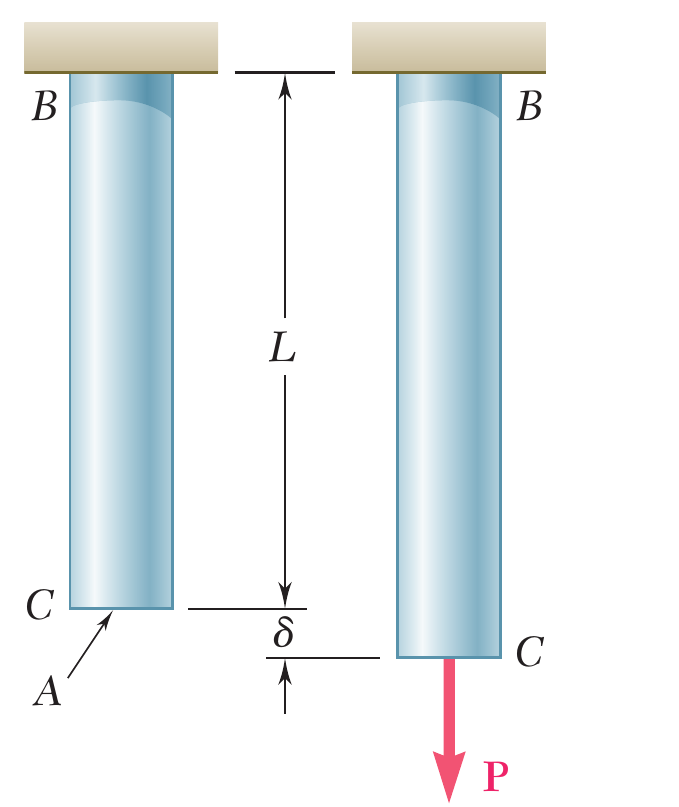
\includegraphics[width=\linewidth,height=4.9cm,keepaspectratio]{Chap_2/fig_2_1.png}\\
      \tiny Hình 2.1
      \[
        \sigma = \frac{P}{A} = \text{ứng suất}
      \]
      \[
        \varepsilon = \frac{\delta}{L} = \text{biến dạng dài tỉ đối}
      \]
    \column{0.32\textwidth}
      \centering
      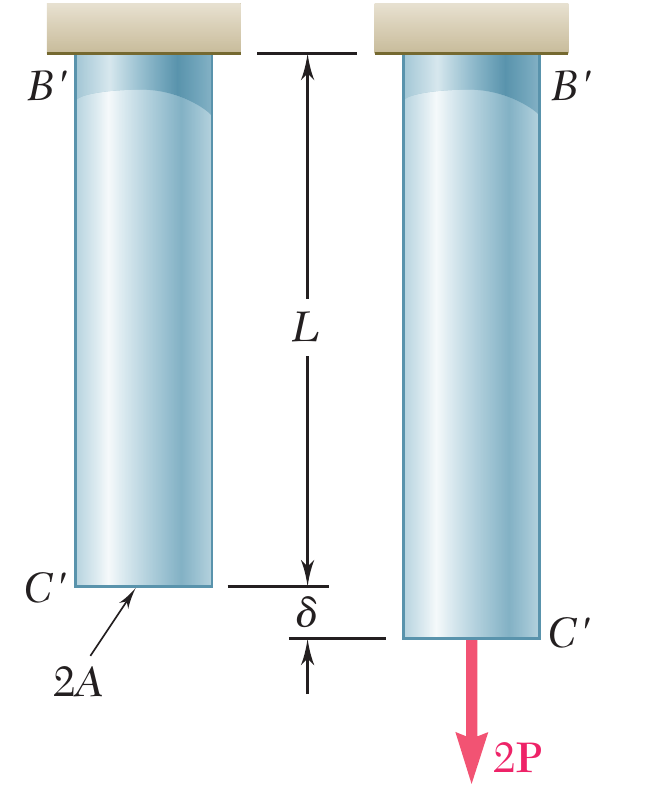
\includegraphics[width=\linewidth,height=4.9cm,keepaspectratio]{Chap_2/fig_2_3.png}\\
      \tiny Hình 2.3
      \[
        \sigma = \frac{2P}{2A} = \frac{P}{A}
      \]
      \[
        \varepsilon = \frac{\delta}{L}
      \]
    \column{0.32\textwidth}
      \centering
      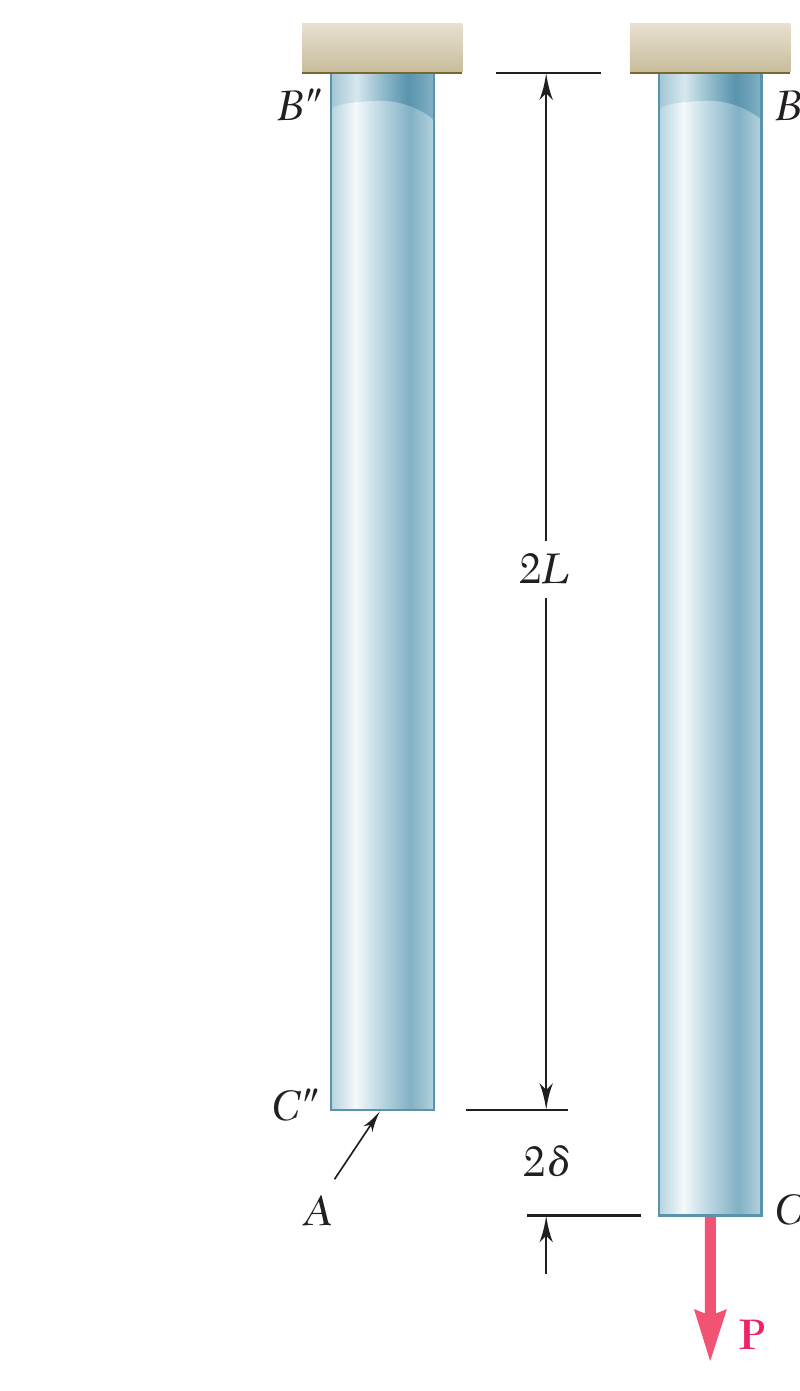
\includegraphics[width=\linewidth,height=4.9cm,keepaspectratio]{Chap_2/fig_2_4.png}\\
      \tiny Hình 2.4
      \[
        \sigma = \frac{P}{A}
      \]
      \[
        \varepsilon = \frac{2\delta}{2L} = \frac{\delta}{L}
      \]
  \end{columns}
\end{frame}
% ===========
\section{Thí nghiệm kéo}
\begin{frame}[t]{Thí nghiệm ứng suất -- biến dạng}
  \begin{columns}[T]
    \column{0.49\textwidth}
      \centering
      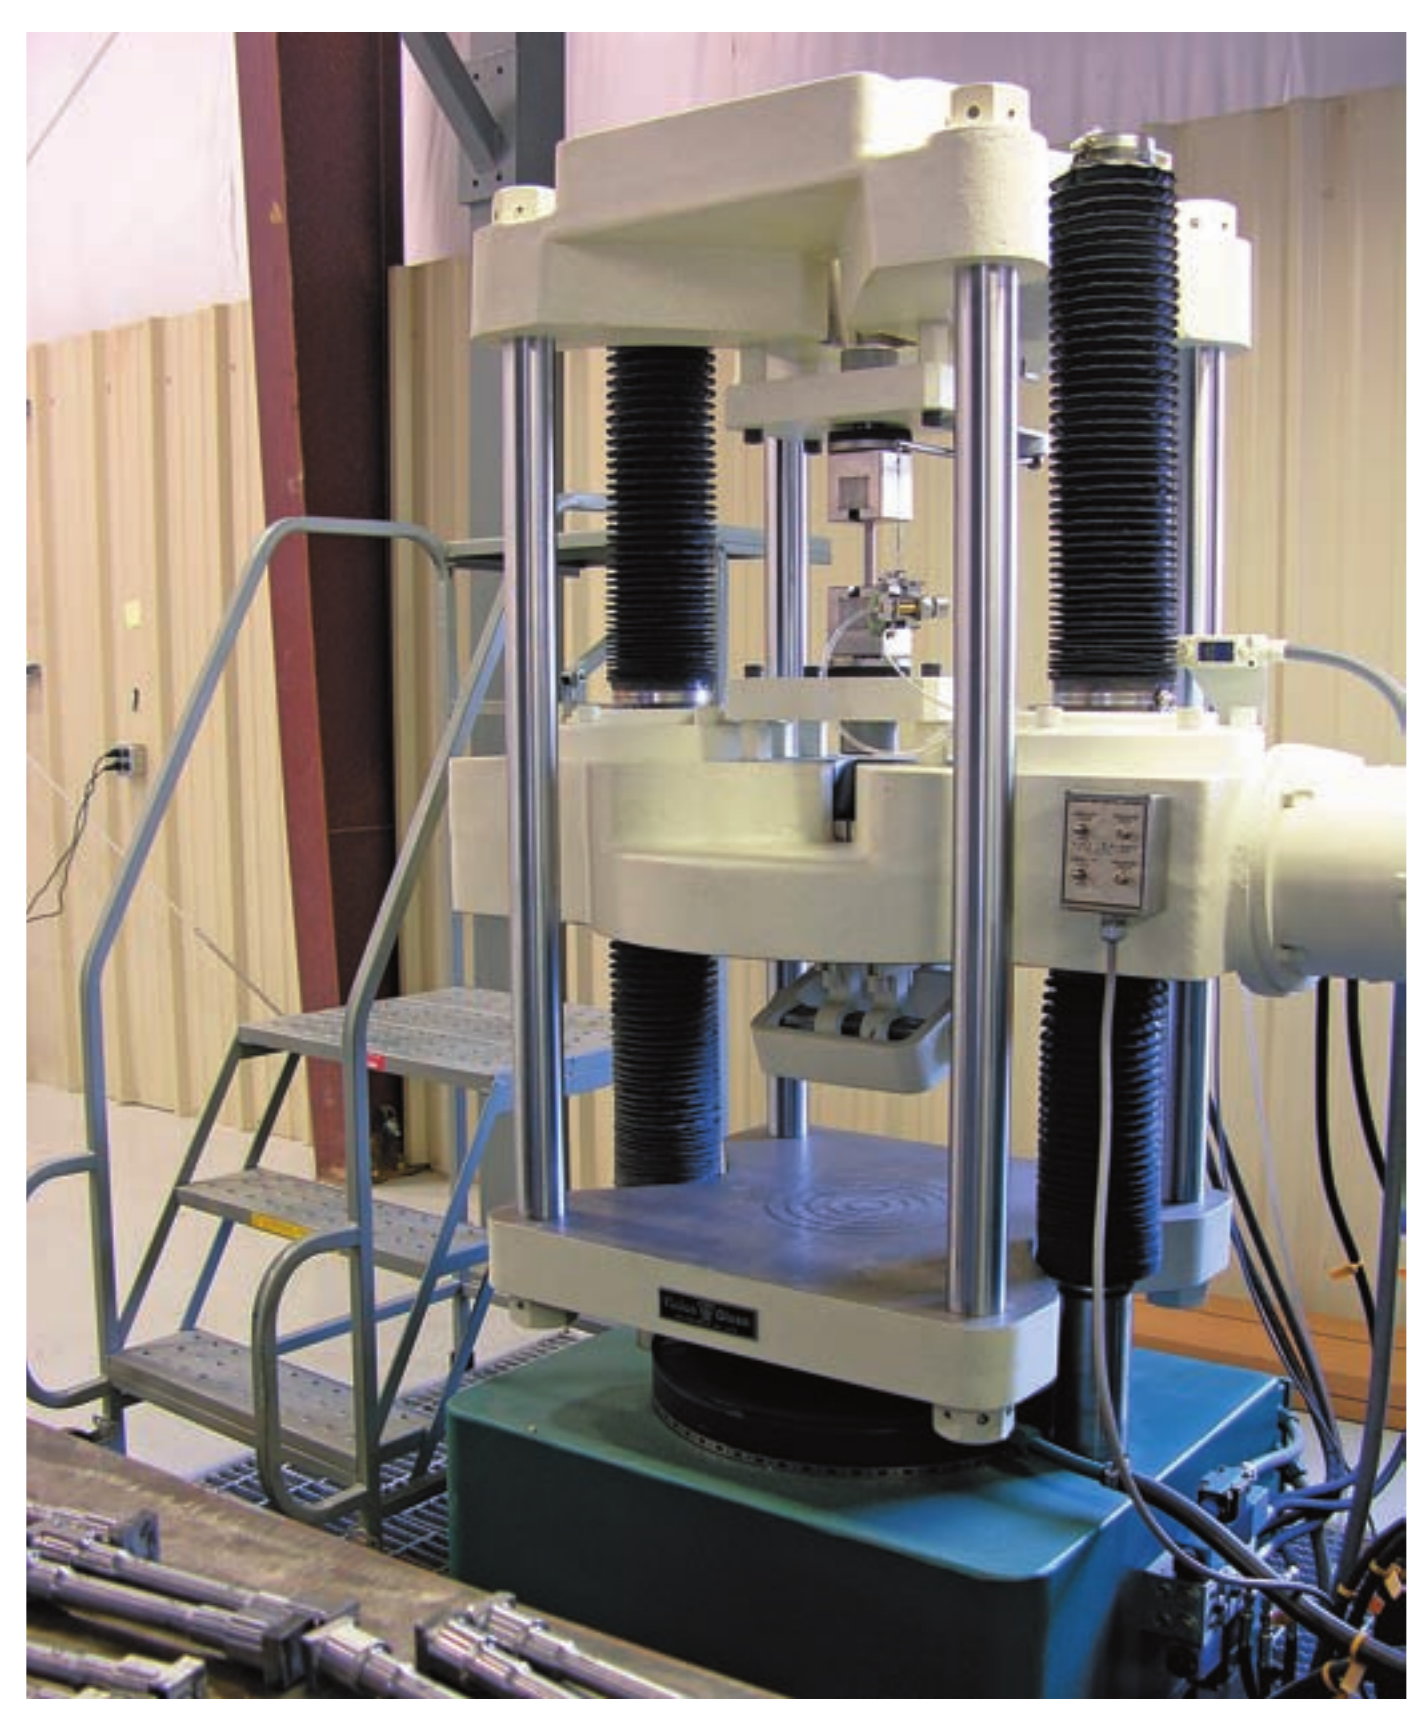
\includegraphics[width=\linewidth,height=5.5cm,keepaspectratio]{Chap_2/photo_2_2.png}\\[0.3em]
      \scriptsize Ảnh 2.2: Máy dùng để thử kéo các mẫu thí nghiệm như
      các mẫu được trình bày trong chương này.
    \column{0.49\textwidth}
      \centering
      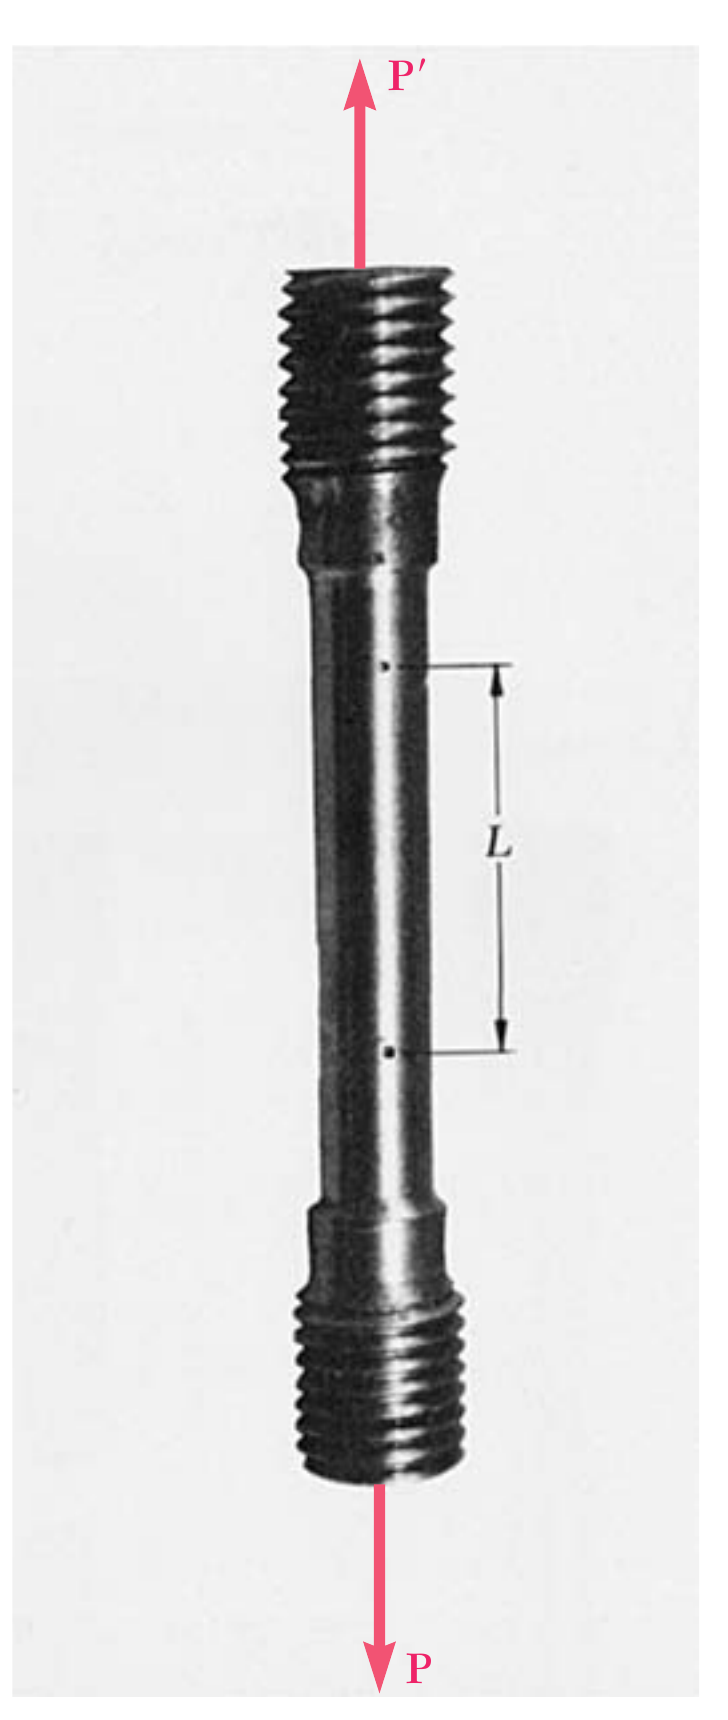
\includegraphics[width=\linewidth,height=5.5cm,keepaspectratio]{Chap_2/photo_2_3.png}\\[0.3em]
      \scriptsize Ảnh 2.3: Mẫu thí nghiệm chịu tải trọng kéo.
  \end{columns}
\end{frame}
% ===========
\section{Biểu đồ ứng suất -- biến dạng: vật liệu dẻo}
\begin{frame}[t]{Biểu đồ ứng suất -- biến dạng: vật liệu dẻo}
  \centering
  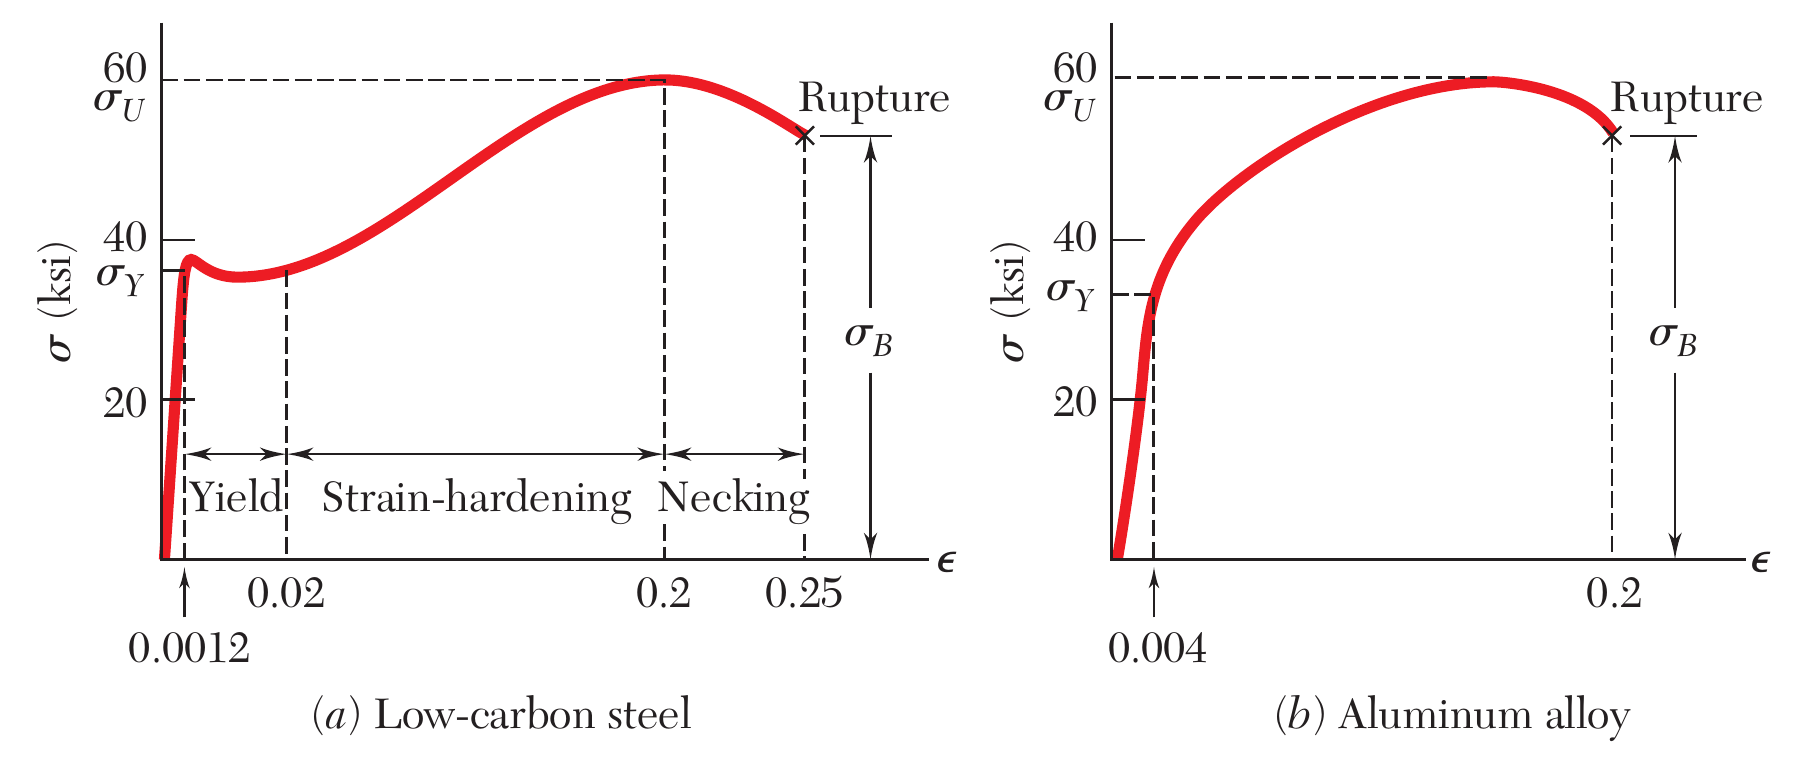
\includegraphics[width=0.9\textwidth,height=6.5cm,keepaspectratio]{Chap_2/fig_2_6.png}
\end{frame}
% ===========
\section{Biểu đồ ứng suất -- biến dạng: vật liệu giòn}
\begin{frame}[t]{Biểu đồ ứng suất -- biến dạng: vật liệu giòn}
  \begin{columns}[T]
    \column{0.49\textwidth}
      \centering
      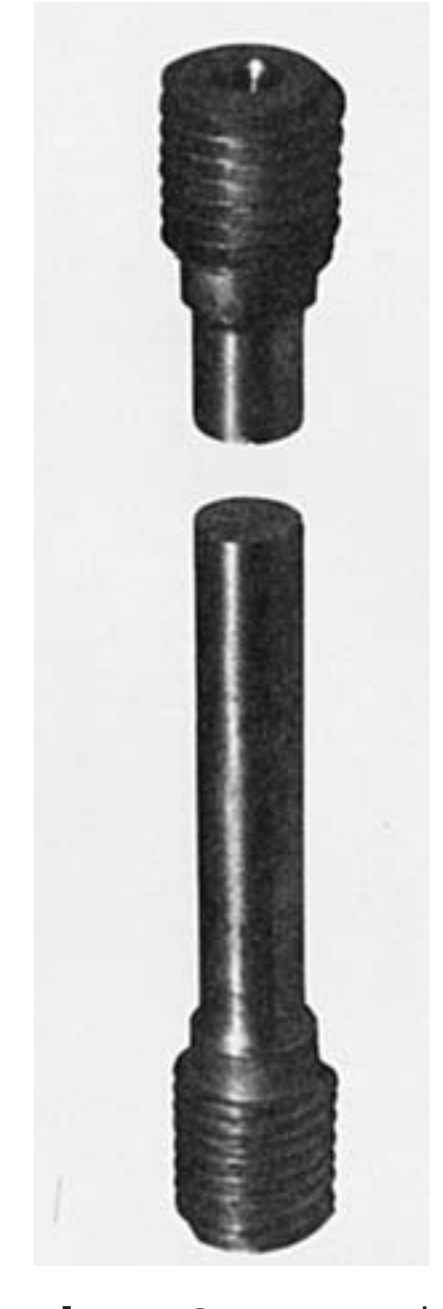
\includegraphics[width=\linewidth,height=5.5cm,keepaspectratio]{Chap_2/photo_2_5.png}
    \column{0.49\textwidth}
      \centering
      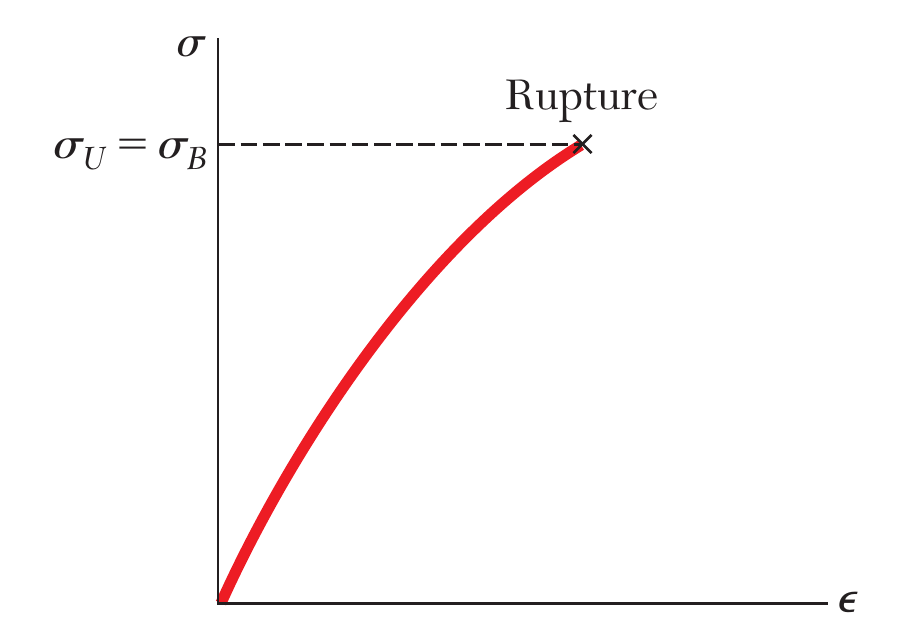
\includegraphics[width=\linewidth,height=5.5cm,keepaspectratio]{Chap_2/fig_2_7.png}\\[0.3em]
      \scriptsize Hình 2.7: Biểu đồ ứng suất -- biến dạng của một vật
      liệu giòn điển hình.
  \end{columns}
\end{frame}
% ===========
\section{Định luật Hooke: mô đun đàn hồi}
\begin{frame}[t]{Định luật Hooke: mô đun đàn hồi}
  \begin{columns}[T]
    \column{0.48\textwidth}
      \small
      \begin{itemize}
        \setlength{\itemsep}{1em}
        \item Khi ứng suất nhỏ hơn giới hạn chảy:
        \[
          \sigma = E\varepsilon
        \]
        $E$ = mô đun Young, hay mô đun đàn hồi.
        \item Độ bền chịu ảnh hưởng của thành phần hợp kim, nhiệt luyện
              và quá trình chế tạo, nhưng độ cứng (mô đun đàn hồi) thì
              không.
      \end{itemize}
    \column{0.50\textwidth}
      \centering
      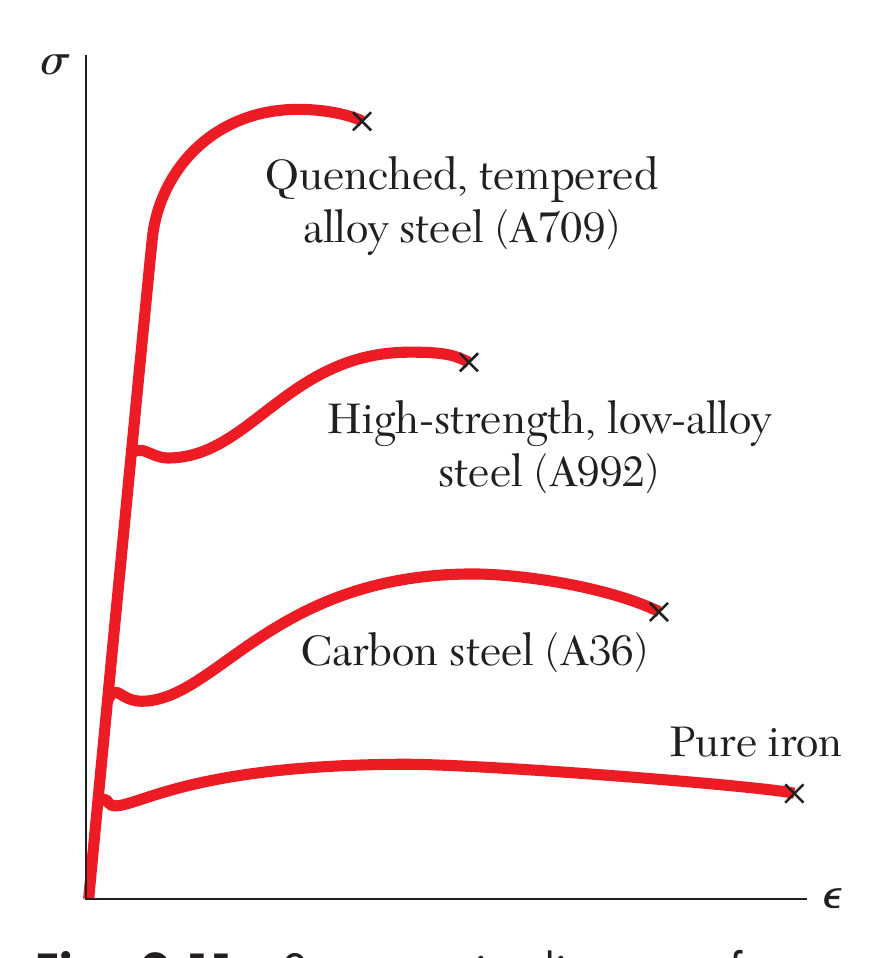
\includegraphics[width=\linewidth,height=5.3cm,keepaspectratio]{Chap_2/fig_2_11.png}\\[0.3em]
      \scriptsize Hình 2.11: Biểu đồ ứng suất -- biến dạng của sắt và
      các mác thép khác nhau.
  \end{columns}
\end{frame}
% ===========
\section{Ứng xử đàn hồi và ứng xử dẻo}
\begin{frame}[t]{Ứng xử đàn hồi và ứng xử dẻo}
  \begin{columns}[T]
    \column{0.52\textwidth}
      \small
      \begin{itemize}
        \setlength{\itemsep}{1em}
        \item Nếu biến dạng biến mất khi bỏ ứng suất, vật liệu được
              gọi là có ứng xử \emph{đàn hồi}.
        \item Ứng suất lớn nhất mà tại đó điều này còn xảy ra được gọi
              là \emph{giới hạn đàn hồi}.
        \item Khi biến dạng không trở về 0 sau khi bỏ ứng suất, vật liệu
              được gọi là có ứng xử \emph{dẻo}.
      \end{itemize}
    \column{0.46\textwidth}
      \centering
      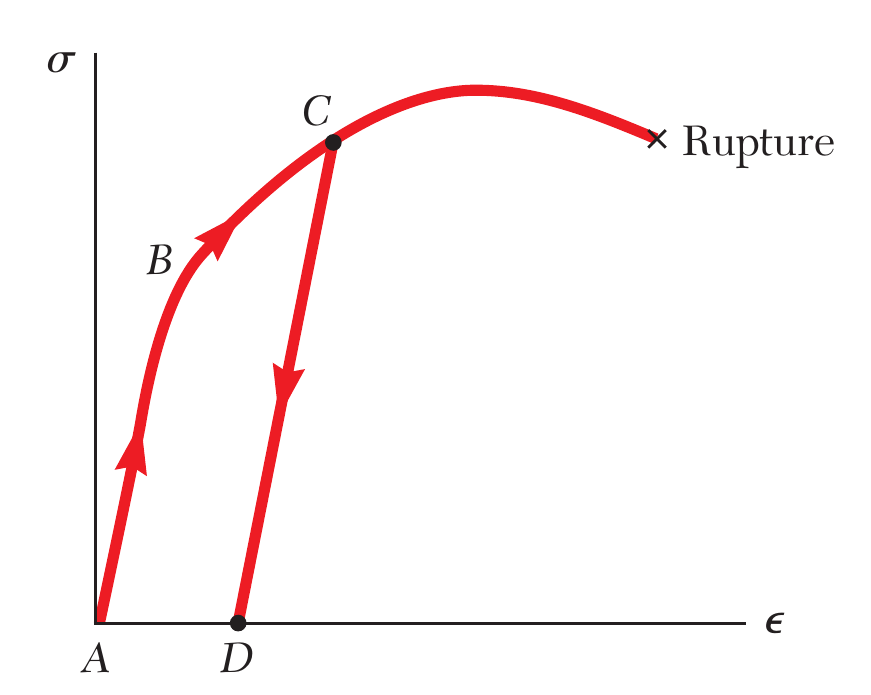
\includegraphics[width=\linewidth,height=5.3cm,keepaspectratio]{Chap_2/fig_2_13.png}\\[0.3em]
      \scriptsize Hình 2.13
  \end{columns}
\end{frame}
% ===========
\section{Mỏi}
\begin{frame}[t]{Mỏi}
  \begin{columns}[T]
    \column{0.52\textwidth}
      \small
      \begin{itemize}
        \setlength{\itemsep}{1em}
        \item Các đặc trưng mỏi được biểu diễn trên biểu đồ S--N
              (ứng suất -- số chu kỳ).
        \item Một cấu kiện có thể bị phá hủy do mỏi ở mức ứng suất thấp
              hơn đáng kể so với giới hạn bền nếu phải chịu nhiều chu kỳ
              tải trọng.
        \item Khi ứng suất giảm xuống dưới \emph{giới hạn mỏi}, phá hủy
              do mỏi không xảy ra với bất kỳ số chu kỳ nào.
      \end{itemize}
    \column{0.46\textwidth}
      \centering
      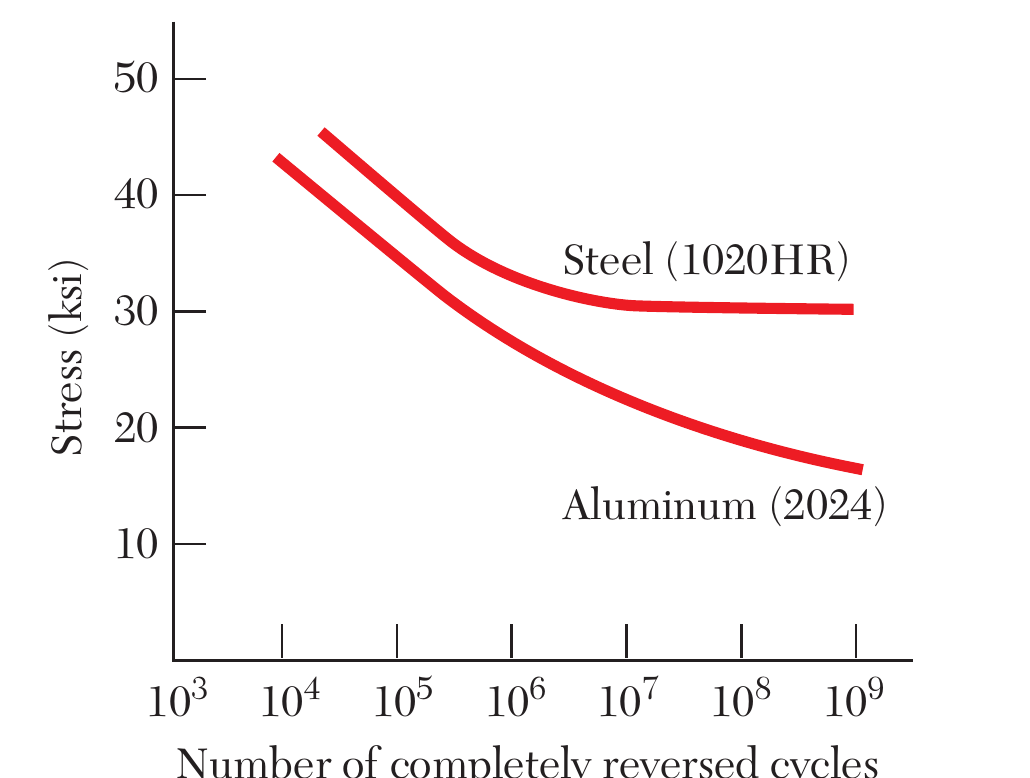
\includegraphics[width=\linewidth,height=5.3cm,keepaspectratio]{Chap_2/fig_2_16.png}
  \end{columns}
\end{frame}
% ===========
\section{Biến dạng dưới tác dụng của tải trọng dọc trục}
\begin{frame}[t]{Biến dạng dưới tác dụng của tải trọng dọc trục}
  \begin{columns}[T]
    \column{0.58\textwidth}
      \small
      \begin{itemize}
        \setlength{\itemsep}{0.5em}
        \item Từ định luật Hooke:
        \[
          \sigma = E\varepsilon \qquad
          \varepsilon = \frac{\sigma}{E} = \frac{P}{AE}
        \]
        \item Từ định nghĩa biến dạng:
        \[
          \varepsilon = \frac{\delta}{L}
        \]
        \item Cân bằng hai biểu thức và giải ra độ biến dạng:
        \[
          \delta = \frac{PL}{AE}
        \]
        \item Khi tải trọng, mặt cắt ngang hoặc đặc tính vật liệu thay
              đổi:
        \[
          \delta = \sum_i \frac{P_i L_i}{A_i E_i}
        \]
      \end{itemize}
    \column{0.40\textwidth}
      \centering
      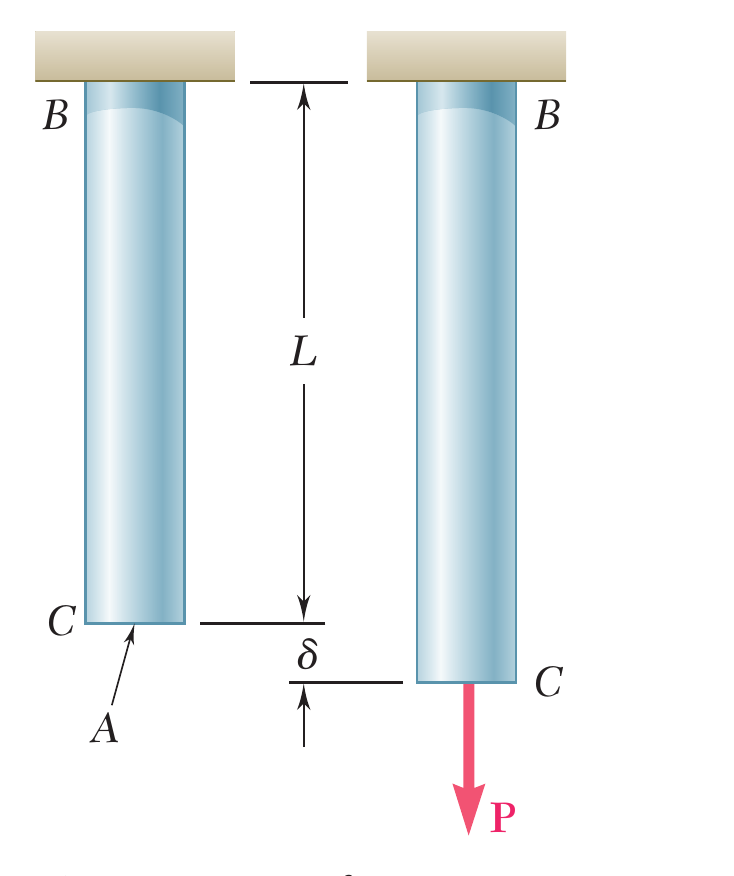
\includegraphics[width=\linewidth,height=5.5cm,keepaspectratio]{Chap_2/fig_2_17.png}\\[0.3em]
      \tiny Hình 2.17
  \end{columns}
\end{frame}
% ===========
\section{Ví dụ 2.01}
\begin{frame}[t]{Ví dụ 2.01}
  \begin{columns}[T]
    \column{0.44\textwidth}
      \centering
      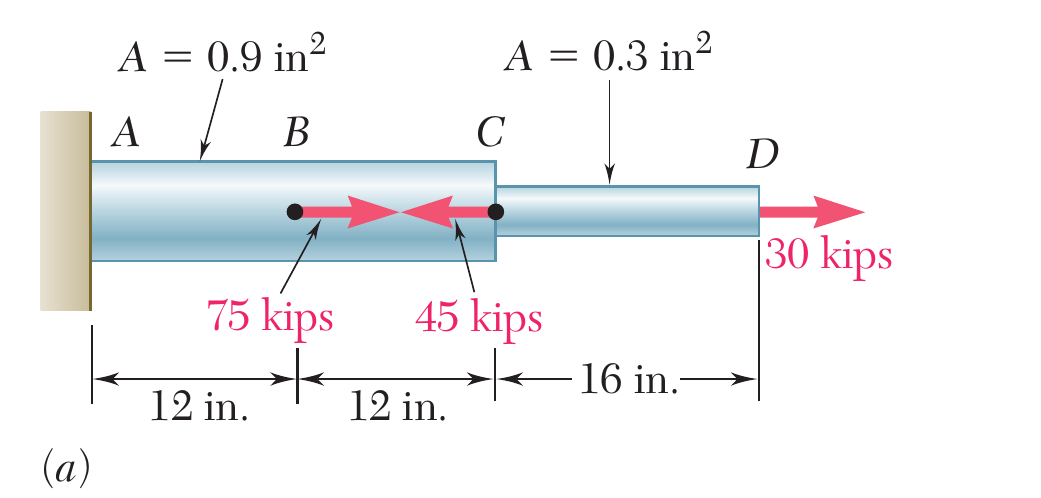
\includegraphics[width=\linewidth,height=2.9cm,keepaspectratio]{Chap_2/fig_2_19a.png}\\[2pt]
      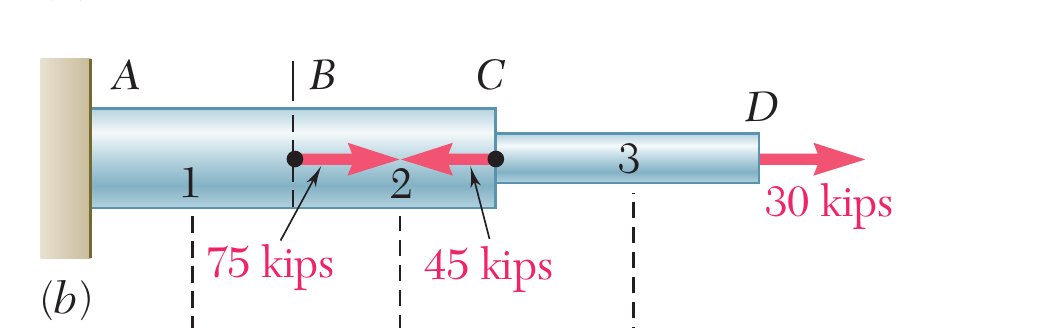
\includegraphics[width=\linewidth,height=2.9cm,keepaspectratio]{Chap_2/fig_2_19b.png}
    \column{0.54\textwidth}
      \small
      Xác định biến dạng của thanh thép như hình vẽ dưới tác dụng của
      các tải trọng đã cho.

      \vspace{0.8em}
      \textbf{LỜI GIẢI:}
      \begin{itemize}
        \setlength{\itemsep}{0.6em}
        \item Chia thanh thành các đoạn tại các điểm đặt tải trọng.
        \item Áp dụng phân tích vật thể tự do cho từng đoạn để xác định
              nội lực.
        \item Tính tổng biến dạng của các đoạn.
      \end{itemize}
  \end{columns}
\end{frame}
% ===========
\begin{frame}[t]{Ví dụ 2.01 (tiếp)}
  \begin{columns}[T]
    \column{0.36\textwidth}
      \centering
      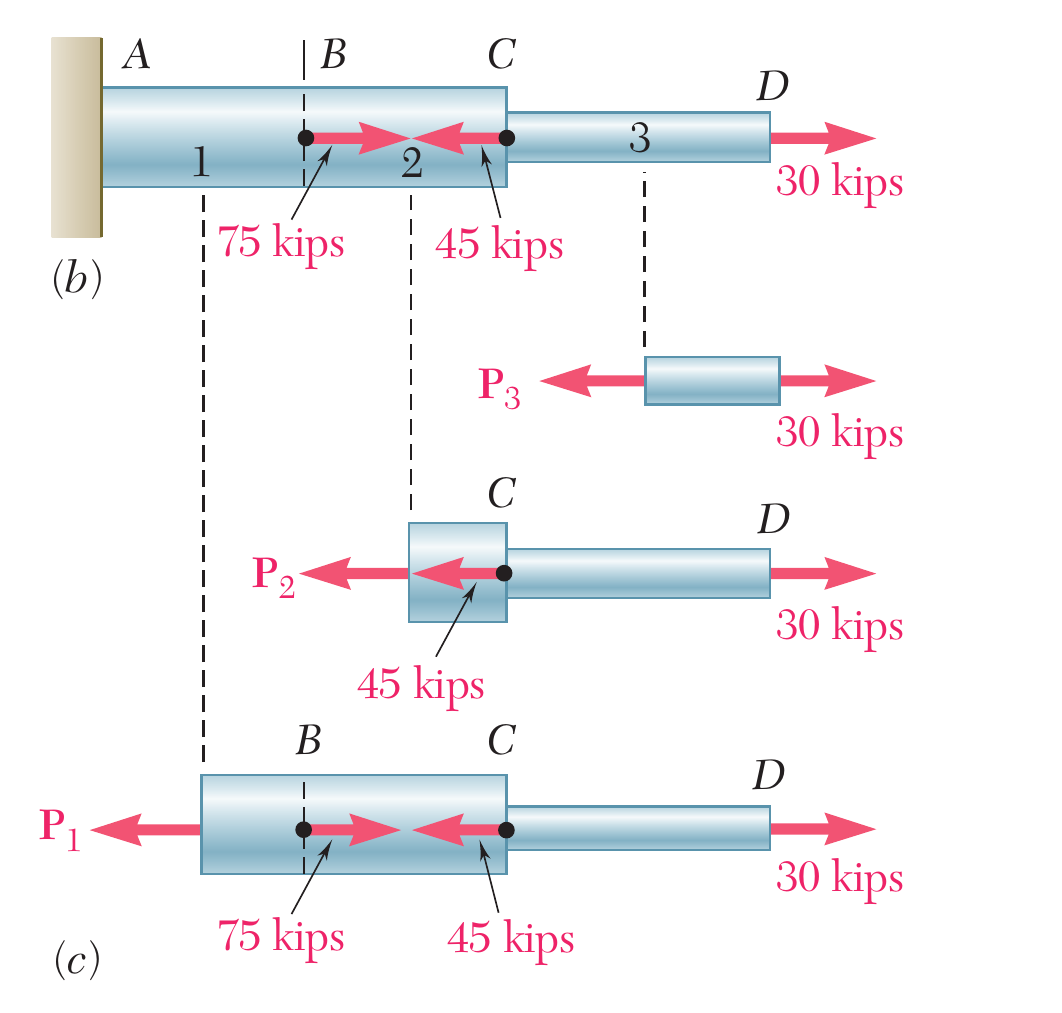
\includegraphics[width=\linewidth,height=7cm,keepaspectratio]{Chap_2/fig_2_19bc.png}
    \column{0.62\textwidth}
      \scriptsize
      \textbf{LỜI GIẢI:}
      \begin{itemize}
        \setlength{\itemsep}{0.25em}
        \item Chia thanh thành ba đoạn:
        \[
          L_1 = L_2 = 0{,}3\,\mathrm{m}, \quad L_3 = 0{,}4\,\mathrm{m}
        \]
        \[
          A_1 = A_2 = 581\times10^{-6}\,\mathrm{m}^2, \quad
          A_3 = 194\times10^{-6}\,\mathrm{m}^2
        \]
        \item Phân tích vật thể tự do cho từng đoạn để xác định nội lực:
        \[
          P_1 = 240\times10^{3}\,\mathrm{N}, \quad
          P_2 = -60\times10^{3}\,\mathrm{N}, \quad
          P_3 = 120\times10^{3}\,\mathrm{N}
        \]
        \item Tính tổng biến dạng:
        \[
          \delta = \sum_i \frac{P_i L_i}{A_i E_i}
          = \frac{1}{E}\left(\frac{P_1L_1}{A_1} + \frac{P_2L_2}{A_2}
            + \frac{P_3L_3}{A_3}\right)
        \]
        \[
          = \frac{1}{200\times10^{9}}\left[
            \frac{(240\times10^{3})0{,}3}{581\times10^{-6}}
          + \frac{(-60\times10^{3})0{,}3}{581\times10^{-6}}\right.
        \]
        \[
          \left.\qquad + \frac{(120\times10^{3})0{,}4}{194\times10^{-6}}\right]
        \]
        \[
          = 1{,}73\times10^{-3}\,\mathrm{m}
          \qquad \boxed{\delta = 1{,}73\,\mathrm{mm}}
        \]
      \end{itemize}
  \end{columns}
\end{frame}
% ===========
\section{Bài mẫu 2.1}
\begin{frame}[t]{Bài mẫu 2.1}
  \begin{columns}[T]
    \column{0.40\textwidth}
      \centering
      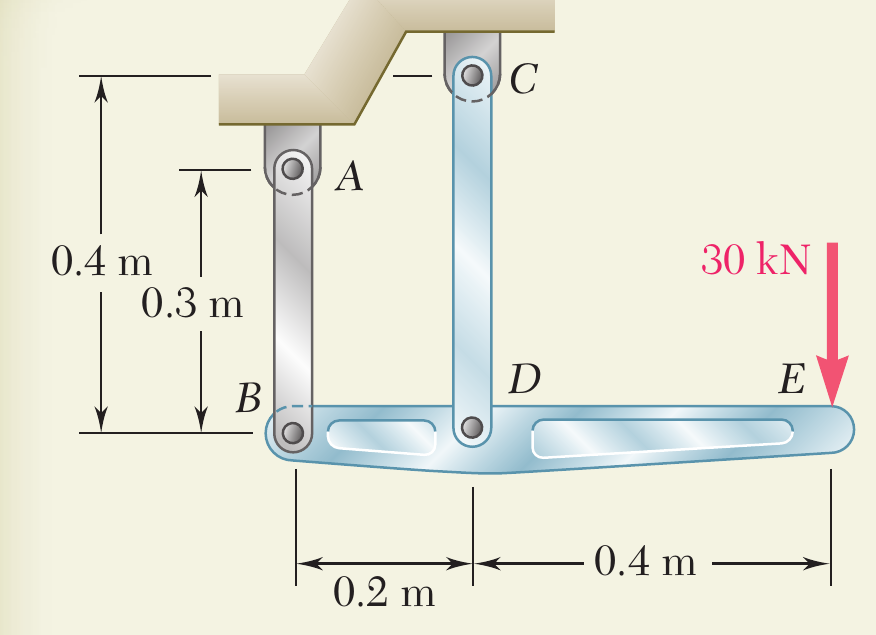
\includegraphics[width=\linewidth,height=5.5cm,keepaspectratio]{Chap_2/sp_2_1_1.png}
    \column{0.58\textwidth}
      \footnotesize
      Thanh cứng $BDE$ được đỡ bởi hai thanh liên kết $AB$ và $CD$.

      Thanh $AB$ bằng nhôm ($E = 70\,\mathrm{GPa}$), diện tích mặt cắt
      ngang $500\,\mathrm{mm}^2$. Thanh $CD$ bằng thép
      ($E = 200\,\mathrm{GPa}$), diện tích mặt cắt ngang
      $600\,\mathrm{mm}^2$.

      Với lực 30 kN như hình vẽ, xác định chuyển vị a) của $B$, b) của
      $D$ và c) của $E$.

      \vspace{0.5em}
      \textbf{LỜI GIẢI:}
      \begin{itemize}
        \setlength{\itemsep}{0.4em}
        \item Phân tích vật thể tự do của thanh $BDE$ để tìm lực do các
              thanh $AB$ và $DC$ tác dụng.
        \item Tính biến dạng của các thanh $AB$ và $DC$, tức là chuyển
              vị của $B$ và $D$.
        \item Dùng quan hệ hình học để tìm chuyển vị tại $E$ từ chuyển
              vị tại $B$ và $D$.
      \end{itemize}
  \end{columns}
\end{frame}
% ===========
\begin{frame}[t]{Bài mẫu 2.1 (tiếp)}
  \begin{columns}[T]
    % ----- Trái: vật thể tự do của thanh BDE -----
    \column{0.44\textwidth}
      \footnotesize
      \textbf{LỜI GIẢI:} Vật thể tự do: thanh $BDE$
      \[
        \begin{aligned}
          \textstyle\sum M_B &= 0 = -(30\,\mathrm{kN}\times0{,}6\,\mathrm{m})
              + F_{CD}\times0{,}2\,\mathrm{m}\\
          F_{CD} &= +90\,\mathrm{kN}\ \text{(kéo)}\\[0.4em]
          \textstyle\sum M_D &= 0 = -(30\,\mathrm{kN}\times0{,}4\,\mathrm{m})
              - F_{AB}\times0{,}2\,\mathrm{m}\\
          F_{AB} &= -60\,\mathrm{kN}\ \text{(nén)}
        \end{aligned}
      \]
      \centering
      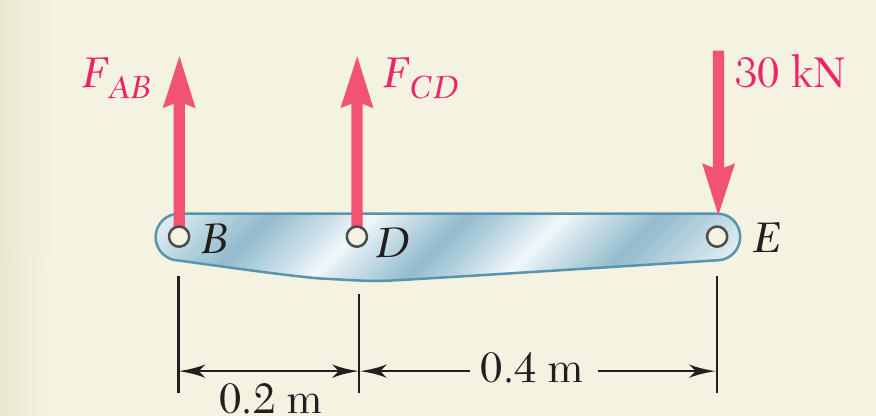
\includegraphics[width=\linewidth,height=2.8cm,keepaspectratio]{Chap_2/sp_2_1_2.png}
    % ----- Phải: chuyển vị của B và D, mỗi phần kèm hình thanh tương ứng -----
    \column{0.54\textwidth}
      \footnotesize
      % --- Chuyển vị của B: hình thanh AB + công thức ---
      \begin{minipage}[c]{0.27\linewidth}
        \centering
        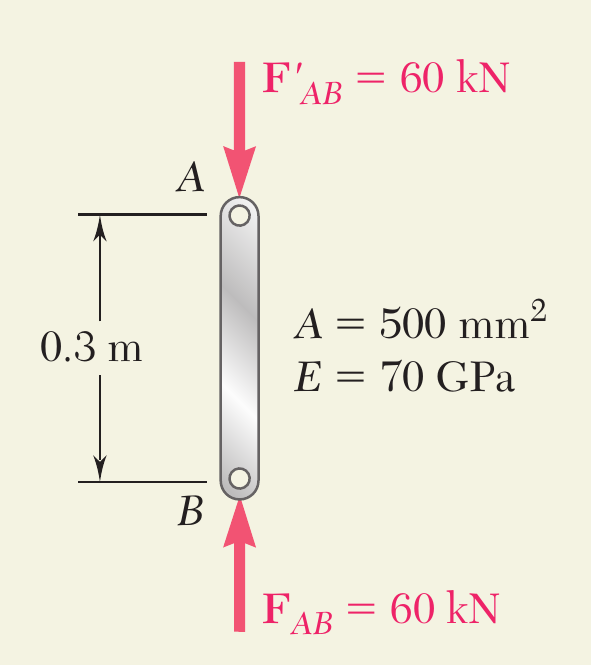
\includegraphics[width=\linewidth,height=3.3cm,keepaspectratio]{Chap_2/sp_2_1_3a.png}
      \end{minipage}\hfill
      \begin{minipage}[c]{0.71\linewidth}
        Chuyển vị của $B$:
        \[
          \delta_B = \frac{PL}{AE}
          = \frac{(-60\times10^{3})(0{,}3)}{(500\times10^{-6})(70\times10^{9})}
        \]
        \[
          \delta_B = -514\times10^{-6}\,\mathrm{m}
        \]
        \[
          \boxed{\delta_B = 0{,}514\,\mathrm{mm}\uparrow}
        \]
      \end{minipage}

      \vspace{0.4em}
      % --- Chuyển vị của D: hình thanh CD + công thức ---
      \begin{minipage}[c]{0.27\linewidth}
        \centering
        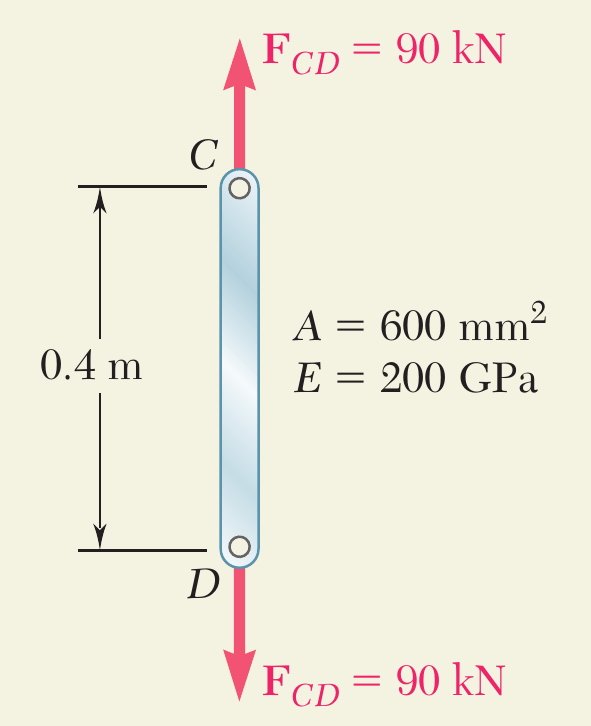
\includegraphics[width=\linewidth,height=3.3cm,keepaspectratio]{Chap_2/sp_2_1_3b.png}
      \end{minipage}\hfill
      \begin{minipage}[c]{0.71\linewidth}
        Chuyển vị của $D$:
        \[
          \delta_D = \frac{PL}{AE}
          = \frac{(90\times10^{3})(0{,}4)}{(600\times10^{-6})(200\times10^{9})}
        \]
        \[
          \delta_D = 300\times10^{-6}\,\mathrm{m}
        \]
        \[
          \boxed{\delta_D = 0{,}300\,\mathrm{mm}\downarrow}
        \]
      \end{minipage}
  \end{columns}
\end{frame}
% ===========
\begin{frame}[t]{Bài mẫu 2.1 (tiếp)}
  \begin{columns}[T]
    \column{0.42\textwidth}
      \centering
      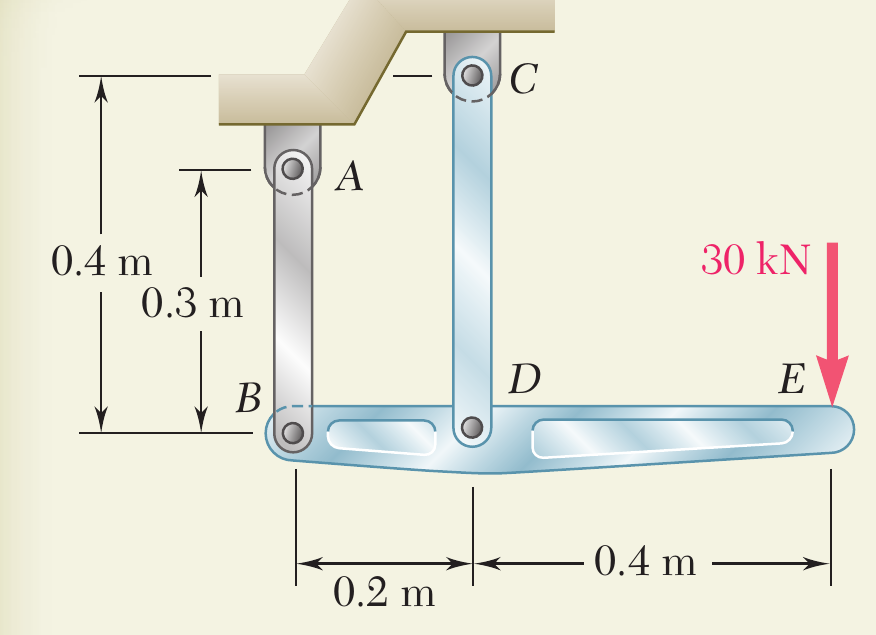
\includegraphics[width=\linewidth,height=2.9cm,keepaspectratio]{Chap_2/sp_2_1_1.png}\\[2pt]
      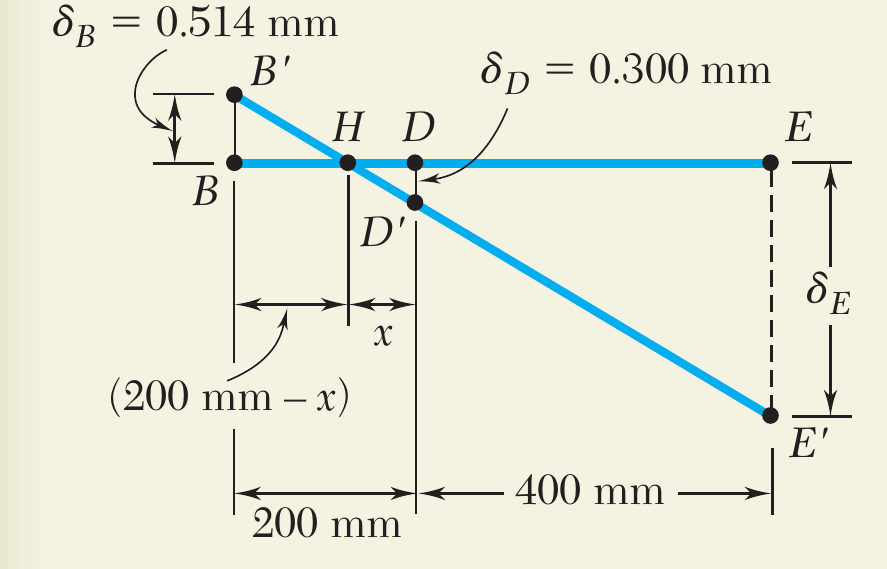
\includegraphics[width=\linewidth,height=2.9cm,keepaspectratio]{Chap_2/sp_2_1_4.png}
    \column{0.56\textwidth}
      \small
      Chuyển vị của $E$ (từ quan hệ tam giác đồng dạng):
      \[
        \frac{BB'}{DD'} = \frac{BH}{HD}
        \quad\Rightarrow\quad
        \frac{0{,}514\,\mathrm{mm}}{0{,}300\,\mathrm{mm}}
          = \frac{(200\,\mathrm{mm}) - x}{x}
      \]
      \[
        x = 73{,}7\,\mathrm{mm}
      \]
      \[
        \frac{EE'}{DD'} = \frac{HE}{HD}
        \quad\Rightarrow\quad
        \frac{\delta_E}{0{,}300\,\mathrm{mm}}
          = \frac{(400 + 73{,}7)\,\mathrm{mm}}{73{,}7\,\mathrm{mm}}
      \]
      \[
        \delta_E = 1{,}928\,\mathrm{mm}
        \qquad \boxed{\delta_E = 1{,}928\,\mathrm{mm}\downarrow}
      \]
  \end{columns}
\end{frame}
% ===========
\section{Bài toán siêu tĩnh}
\begin{frame}[t]{Bài toán siêu tĩnh}
  \begin{columns}[T]
    \column{0.58\textwidth}
      \small
      \begin{itemize}
        \setlength{\itemsep}{0.5em}
        \item Các kết cấu mà nội lực và phản lực không thể xác định chỉ
              bằng tĩnh học được gọi là kết cấu \emph{siêu tĩnh}.
        \item Một kết cấu sẽ là siêu tĩnh khi nó có nhiều liên kết hơn
              số liên kết cần thiết để duy trì cân bằng.
        \item Các phản lực thừa được thay bằng các lực chưa biết; cùng
              với các tải trọng khác, chúng phải gây ra các biến dạng
              tương thích.
        \item Biến dạng do tải trọng thực và do các phản lực thừa được
              xác định riêng rẽ rồi cộng lại (nguyên lý cộng tác dụng):
        \[
          \delta = \delta_L + \delta_R = 0
        \]
      \end{itemize}
    \column{0.40\textwidth}
      \centering
      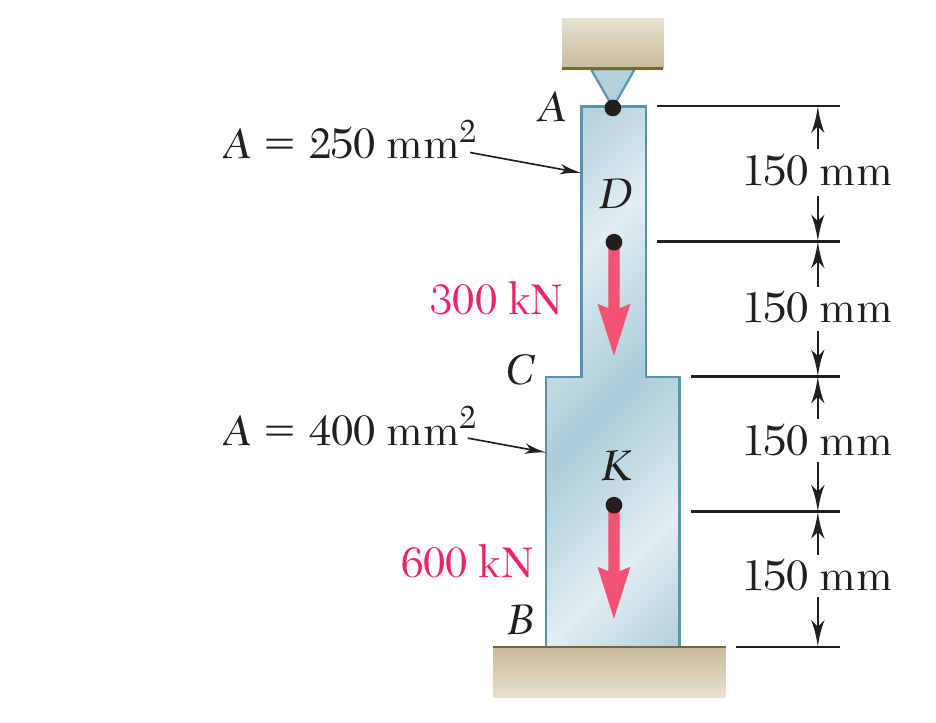
\includegraphics[width=\linewidth,height=2.9cm,keepaspectratio]{Chap_2/fig_2_24.png}\\[2pt]
      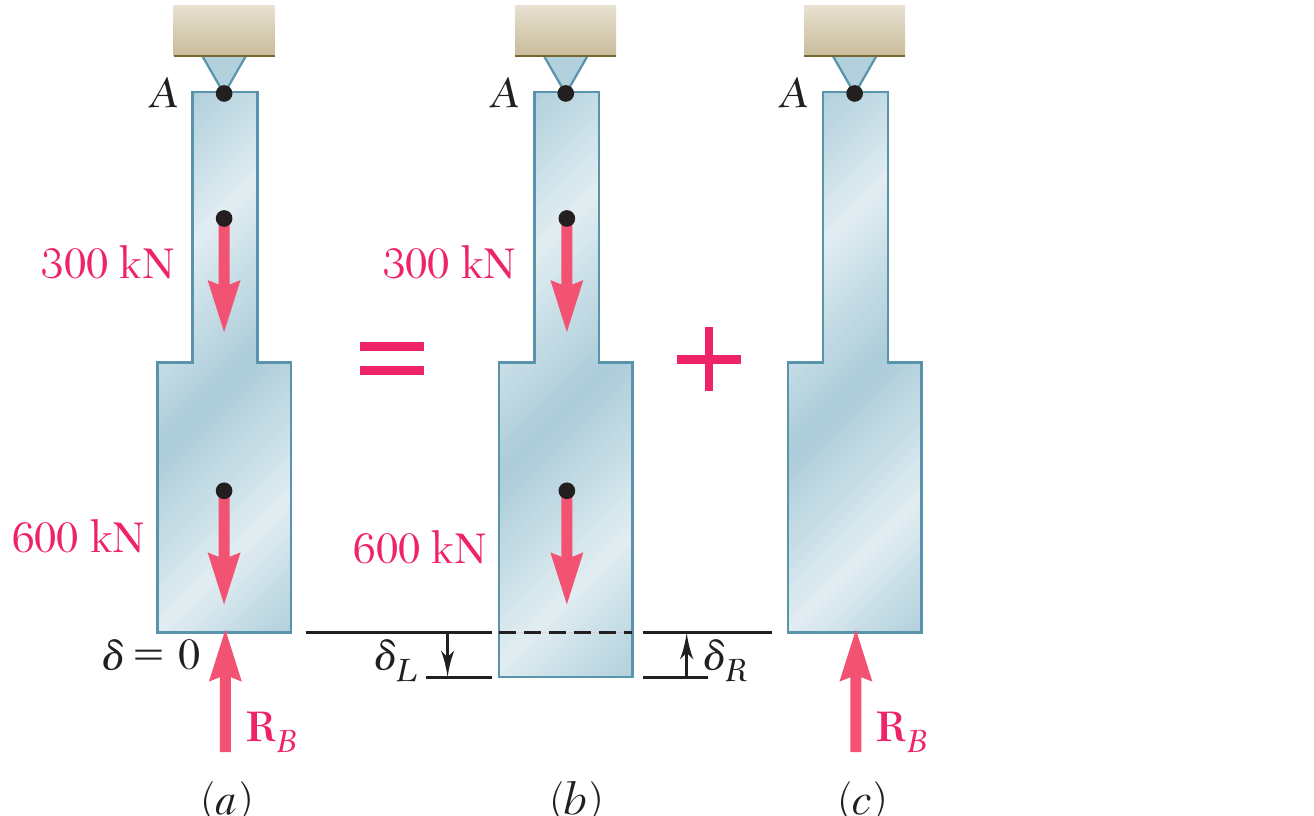
\includegraphics[width=\linewidth,height=2.9cm,keepaspectratio]{Chap_2/fig_2_25.png}
  \end{columns}
\end{frame}
% ===========
\section{Ví dụ 2.04}
\begin{frame}[t]{Ví dụ 2.04}
  \begin{columns}[T]
    \column{0.38\textwidth}
      \centering
      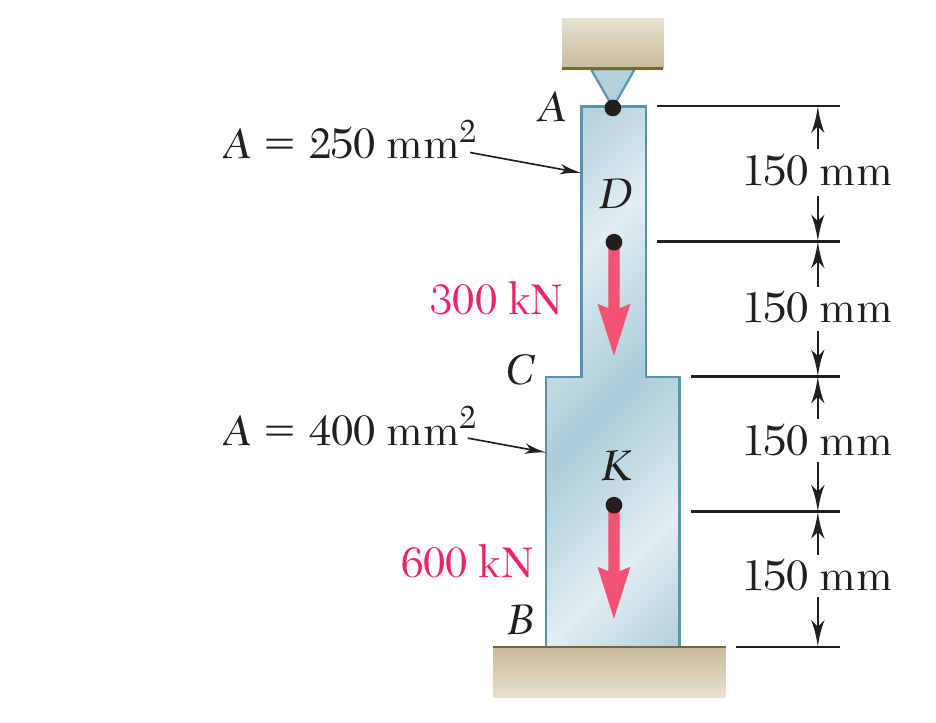
\includegraphics[width=\linewidth,height=2.9cm,keepaspectratio]{Chap_2/fig_2_24.png}\\[2pt]
      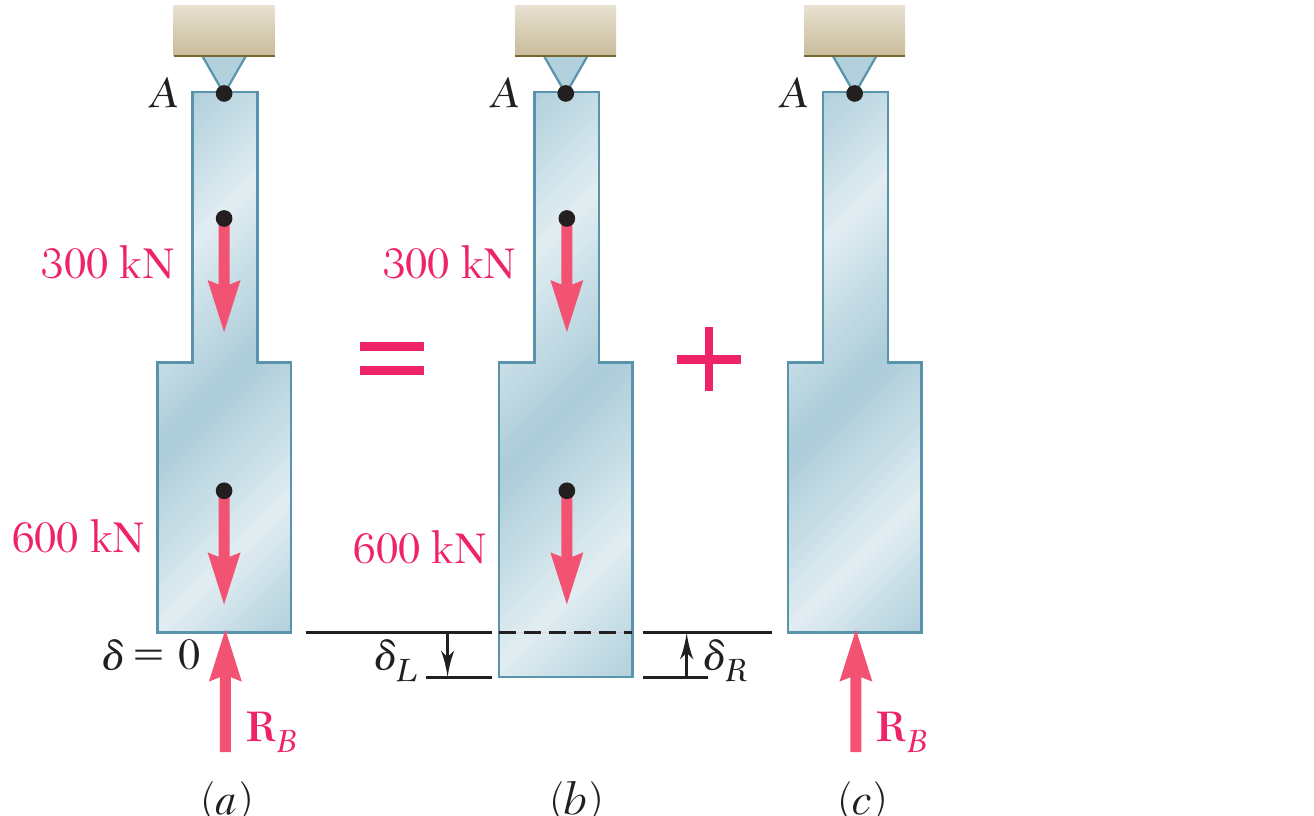
\includegraphics[width=\linewidth,height=2.9cm,keepaspectratio]{Chap_2/fig_2_25.png}
    \column{0.60\textwidth}
      \footnotesize
      Xác định phản lực tại $A$ và $B$ của thanh thép chịu tải như hình
      vẽ, giả thiết thanh vừa khít với cả hai gối trước khi đặt tải.

      \vspace{0.5em}
      \textbf{LỜI GIẢI:}
      \begin{itemize}
        \setlength{\itemsep}{0.4em}
        \item Coi phản lực tại $B$ là phản lực thừa, giải phóng thanh
              khỏi gối đó và tính chuyển vị tại $B$ do tải trọng gây ra.
        \item Tính chuyển vị tại $B$ do phản lực thừa tại $B$ gây ra.
        \item Yêu cầu các chuyển vị do tải trọng và do phản lực thừa
              phải tương thích, tức là tổng của chúng bằng 0.
        \item Tính phản lực tại $A$ từ tải trọng và phản lực $B$ vừa tìm
              được.
      \end{itemize}
  \end{columns}
\end{frame}
% ===========
\begin{frame}[t]{Ví dụ 2.04 (tiếp)}
  \begin{columns}[T]
    \column{0.30\textwidth}
      \centering
      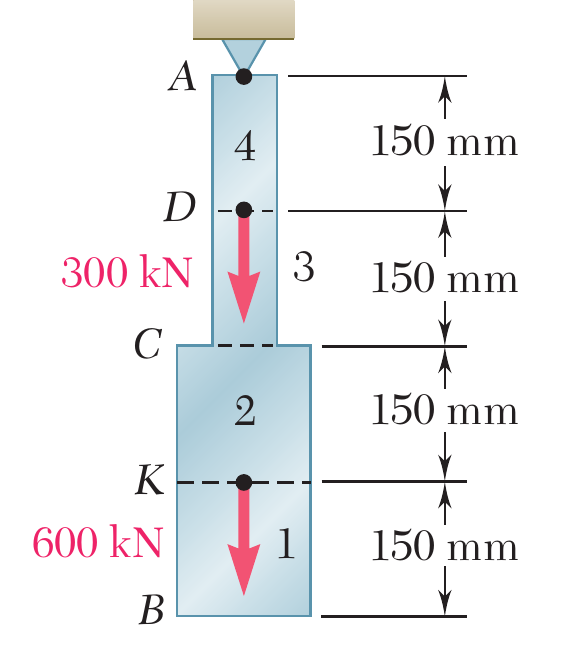
\includegraphics[width=\linewidth,height=2.9cm,keepaspectratio]{Chap_2/fig_2_26.png}\\[2pt]
      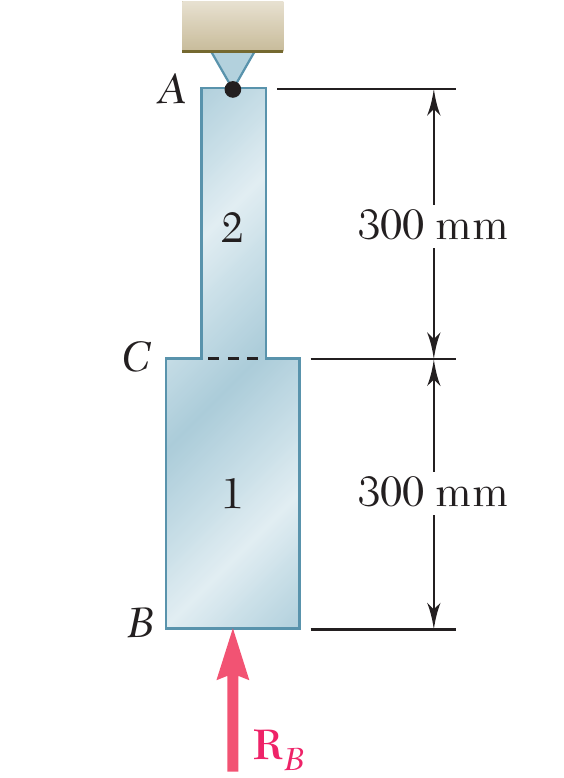
\includegraphics[width=\linewidth,height=2.9cm,keepaspectratio]{Chap_2/fig_2_27.png}
    \column{0.68\textwidth}
      \footnotesize
      \begin{itemize}
        \setlength{\itemsep}{0.3em}
        \item Tính chuyển vị tại $B$ do tải trọng khi đã bỏ liên kết thừa:
        \[
          P_1 = 0, \quad P_2 = P_3 = 600\times10^{3}\,\mathrm{N}, \quad
          P_4 = 900\times10^{3}\,\mathrm{N}
        \]
        \[
          A_1 = A_2 = 400\times10^{-6}\,\mathrm{m}^2, \quad
          A_3 = A_4 = 250\times10^{-6}\,\mathrm{m}^2
        \]
        \[
          L_1 = L_2 = L_3 = L_4 = 0{,}150\,\mathrm{m}
        \]
        \[
          \delta_L = \sum_i \frac{P_iL_i}{A_iE_i}
                   = \frac{1{,}125\times10^{9}}{E}
        \]
        \item Tính chuyển vị tại $B$ do phản lực thừa:
        \[
          P_1 = P_2 = -R_B, \quad L_1 = L_2 = 0{,}300\,\mathrm{m}
        \]
        \[
          A_1 = 400\times10^{-6}\,\mathrm{m}^2, \quad
          A_2 = 250\times10^{-6}\,\mathrm{m}^2
        \]
        \[
          \delta_R = \sum_i \frac{P_iL_i}{A_iE_i}
                   = -\frac{(1{,}95\times10^{3})R_B}{E}
        \]
      \end{itemize}
  \end{columns}
\end{frame}
% ===========
\begin{frame}[t]{Ví dụ 2.04 (tiếp)}
  \begin{columns}[T]
    \column{0.36\textwidth}
      \centering
      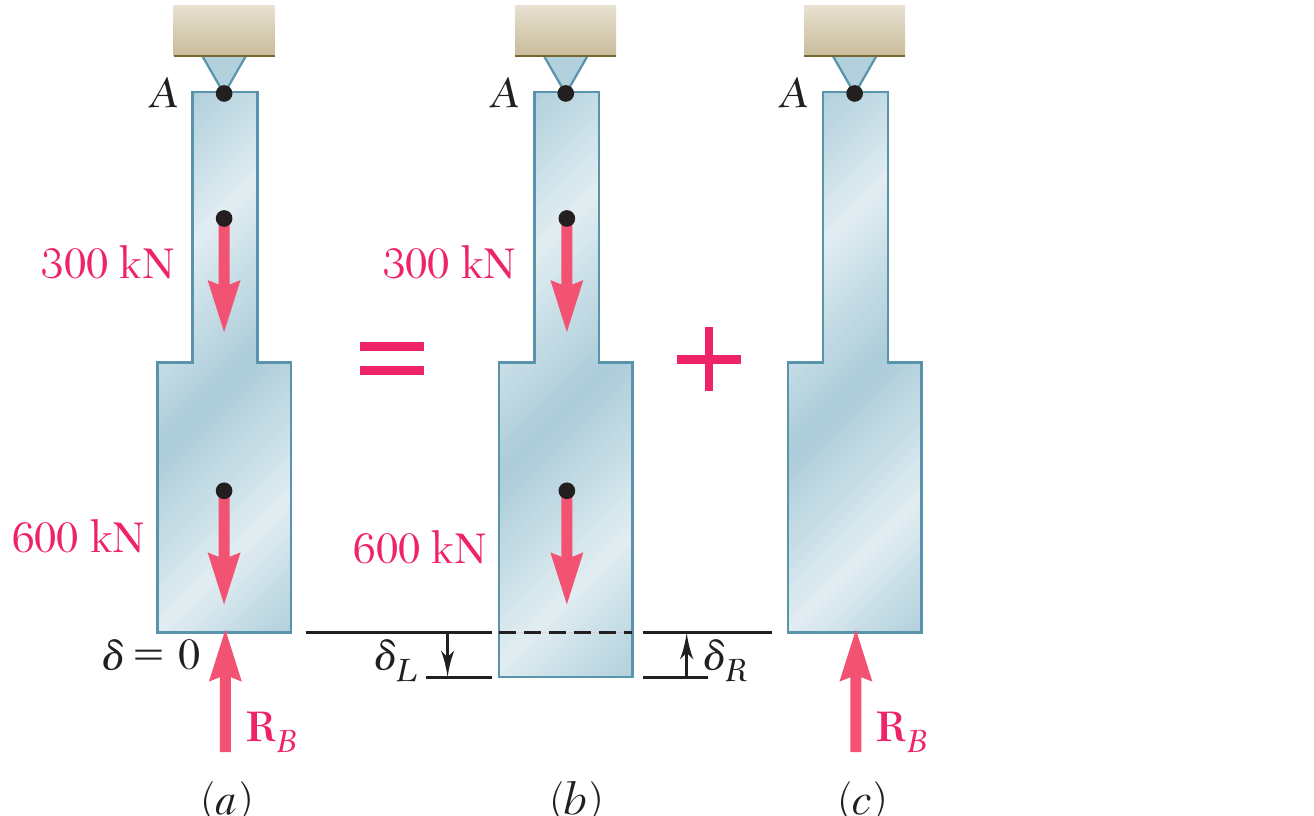
\includegraphics[width=\linewidth,height=2.9cm,keepaspectratio]{Chap_2/fig_2_25.png}\\[2pt]
      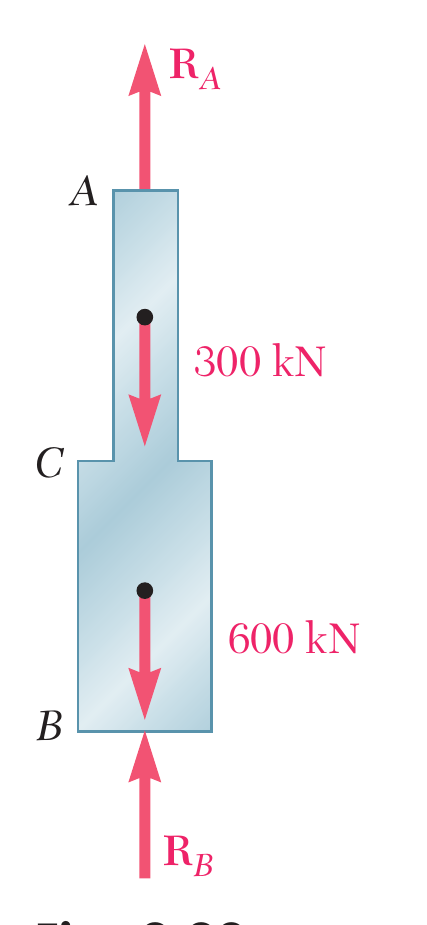
\includegraphics[width=\linewidth,height=2.9cm,keepaspectratio]{Chap_2/fig_2_28.png}
    \column{0.62\textwidth}
      \small
      \begin{itemize}
        \setlength{\itemsep}{0.6em}
        \item Yêu cầu chuyển vị do tải trọng và do phản lực thừa tương
              thích:
        \[
          \delta = \delta_L + \delta_R = 0
        \]
        \[
          \delta = \frac{1{,}125\times10^{9}}{E}
                 - \frac{(1{,}95\times10^{3})R_B}{E} = 0
        \]
        \[
          R_B = 577\times10^{3}\,\mathrm{N} = 577\,\mathrm{kN}
        \]
        \item Tìm phản lực tại $A$ từ tải trọng và phản lực tại $B$:
        \[
          \textstyle\sum F_y = 0 = R_A - 300\,\mathrm{kN} - 600\,\mathrm{kN}
              + 577\,\mathrm{kN}
        \]
        \[
          \boxed{R_A = 323\,\mathrm{kN}, \qquad R_B = 577\,\mathrm{kN}}
        \]
      \end{itemize}
  \end{columns}
\end{frame}
% ===========
\section{Ứng suất nhiệt}
\begin{frame}[t]{Ứng suất nhiệt}
  \begin{columns}[T]
    \column{0.36\textwidth}
      \centering
      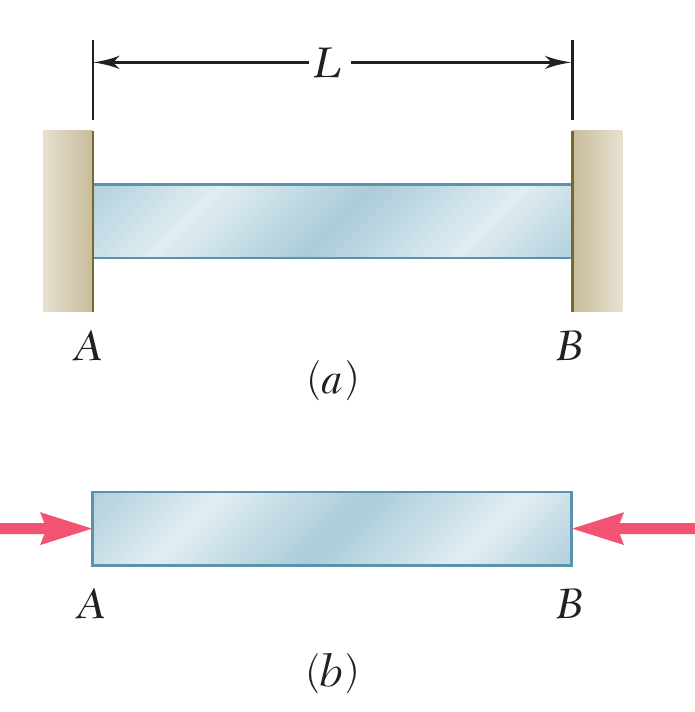
\includegraphics[width=\linewidth,height=2.9cm,keepaspectratio]{Chap_2/fig_2_31.png}\\[2pt]
      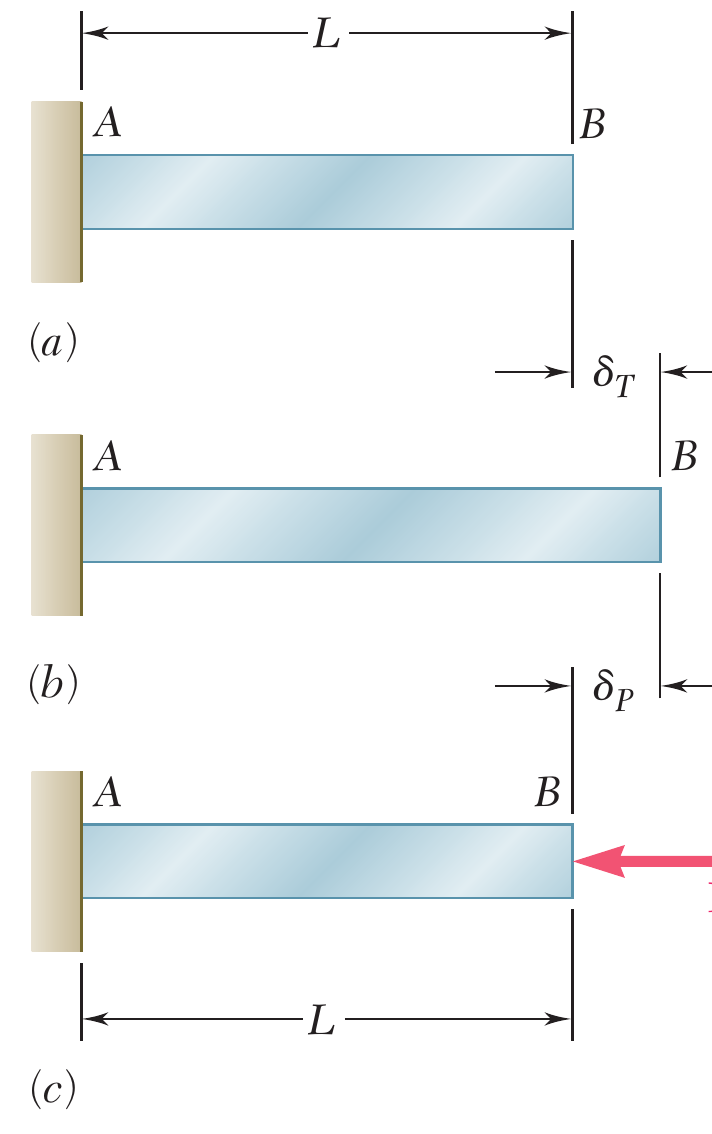
\includegraphics[width=\linewidth,height=2.9cm,keepaspectratio]{Chap_2/fig_2_32.png}
    \column{0.62\textwidth}
      \small
      \begin{itemize}
        \setlength{\itemsep}{0.5em}
        \item Sự thay đổi nhiệt độ làm thay đổi chiều dài, gọi là biến
              dạng nhiệt. Biến dạng nhiệt không gây ra ứng suất trừ khi
              sự giãn dài bị các gối đỡ ngăn cản.
        \item Coi gối đỡ bổ sung là liên kết thừa và áp dụng nguyên lý
              cộng tác dụng:
        \[
          \delta_T = \alpha(\Delta T)L \qquad
          \delta_P = \frac{PL}{AE}
        \]
        $\alpha$ = hệ số giãn nở nhiệt.
        \item Biến dạng nhiệt và biến dạng do liên kết thừa phải tương
              thích:
        \[
          \delta = \delta_T + \delta_P = 0
          \quad\Rightarrow\quad
          \alpha(\Delta T)L + \frac{PL}{AE} = 0
        \]
        \[
          P = -AE\alpha(\Delta T) \qquad
          \sigma = \frac{P}{A} = -E\alpha(\Delta T)
        \]
      \end{itemize}
  \end{columns}
\end{frame}
% ===========
\section{Hệ số Poisson}
\begin{frame}[t]{Hệ số Poisson}
  \begin{columns}[T]
    \column{0.58\textwidth}
      \small
      \begin{itemize}
        \setlength{\itemsep}{0.7em}
        \item Với thanh mảnh chịu tải trọng dọc trục:
        \[
          \varepsilon_x = \frac{\sigma_x}{E} \qquad \sigma_y = \sigma_z = 0
        \]
        \item Sự giãn dài theo phương $x$ đi kèm với sự co ngắn theo các
              phương khác. Giả thiết vật liệu là đẳng hướng (tính chất
              không phụ thuộc phương):
        \[
          \varepsilon_y = \varepsilon_z \neq 0
        \]
        \item Hệ số Poisson được định nghĩa là:
        \[
          \nu = \left|\frac{\text{biến dạng ngang}}{\text{biến dạng dọc}}\right|
              = -\frac{\varepsilon_y}{\varepsilon_x}
              = -\frac{\varepsilon_z}{\varepsilon_x}
        \]
      \end{itemize}
    \column{0.40\textwidth}
      \centering
      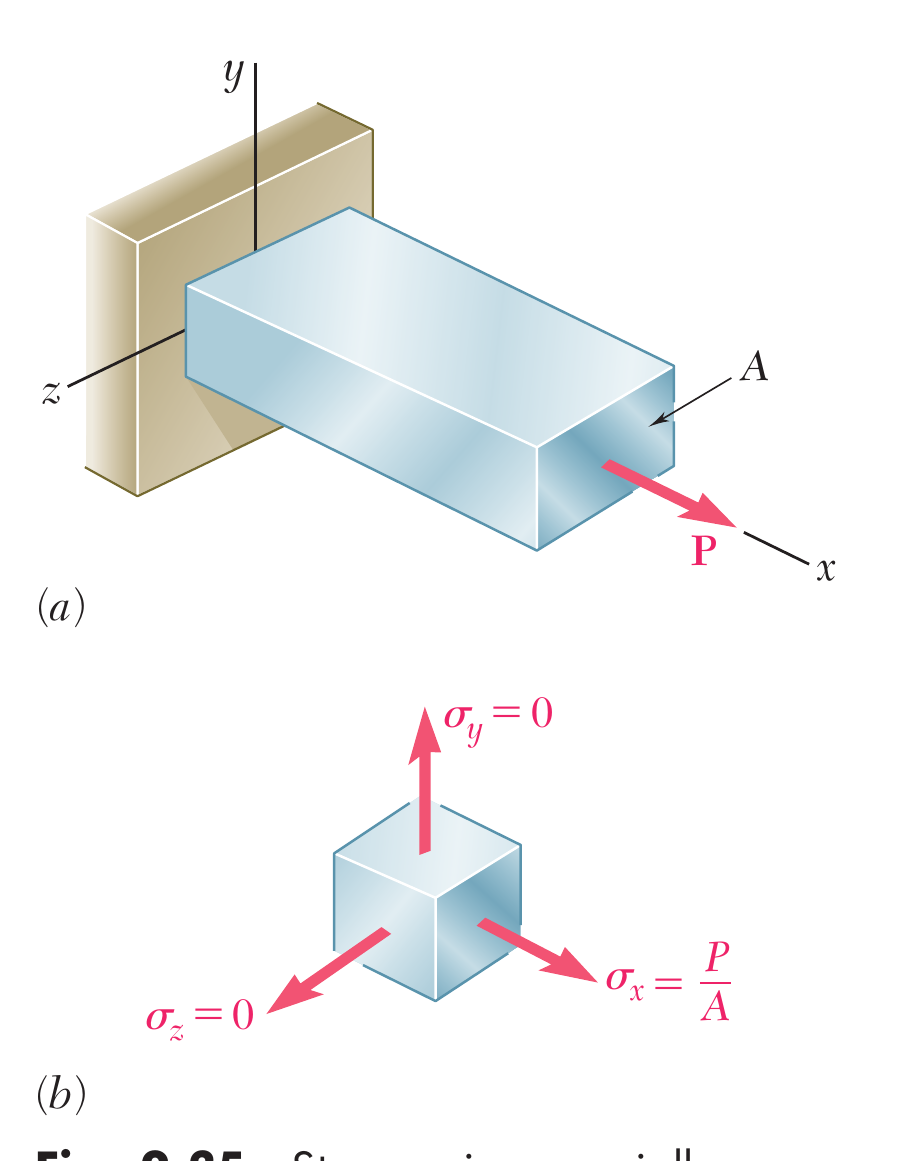
\includegraphics[width=\linewidth,height=2.9cm,keepaspectratio]{Chap_2/fig_2_35.png}\\[2pt]
      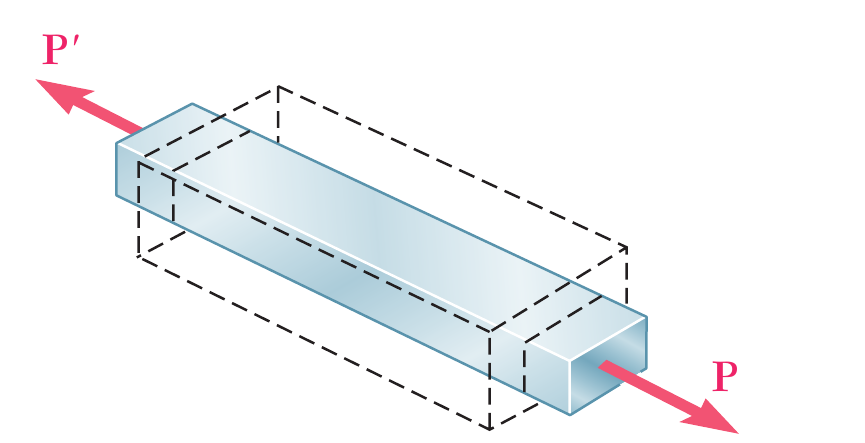
\includegraphics[width=\linewidth,height=2.9cm,keepaspectratio]{Chap_2/fig_2_36.png}
  \end{columns}
\end{frame}
% ===========
\section{Định luật Hooke tổng quát}
\begin{frame}[t]{Định luật Hooke tổng quát}
  \begin{columns}[T]
    \column{0.60\textwidth}
      \small
      \begin{itemize}
        \setlength{\itemsep}{0.6em}
        \item Với phân tố chịu tải trọng nhiều phương, các thành phần
              biến dạng dài do các thành phần ứng suất gây ra có thể xác
              định theo nguyên lý cộng tác dụng. Điều này đòi hỏi:
              \begin{enumerate}
                \item biến dạng quan hệ tuyến tính với ứng suất
                \item biến dạng là nhỏ
              \end{enumerate}
        \item Với các giới hạn trên:
        \[
          \begin{aligned}
            \varepsilon_x &= +\frac{\sigma_x}{E} - \frac{\nu\sigma_y}{E}
                             - \frac{\nu\sigma_z}{E}\\
            \varepsilon_y &= -\frac{\nu\sigma_x}{E} + \frac{\sigma_y}{E}
                             - \frac{\nu\sigma_z}{E}\\
            \varepsilon_z &= -\frac{\nu\sigma_x}{E} - \frac{\nu\sigma_y}{E}
                             + \frac{\sigma_z}{E}
          \end{aligned}
        \]
      \end{itemize}
    \column{0.38\textwidth}
      \centering
      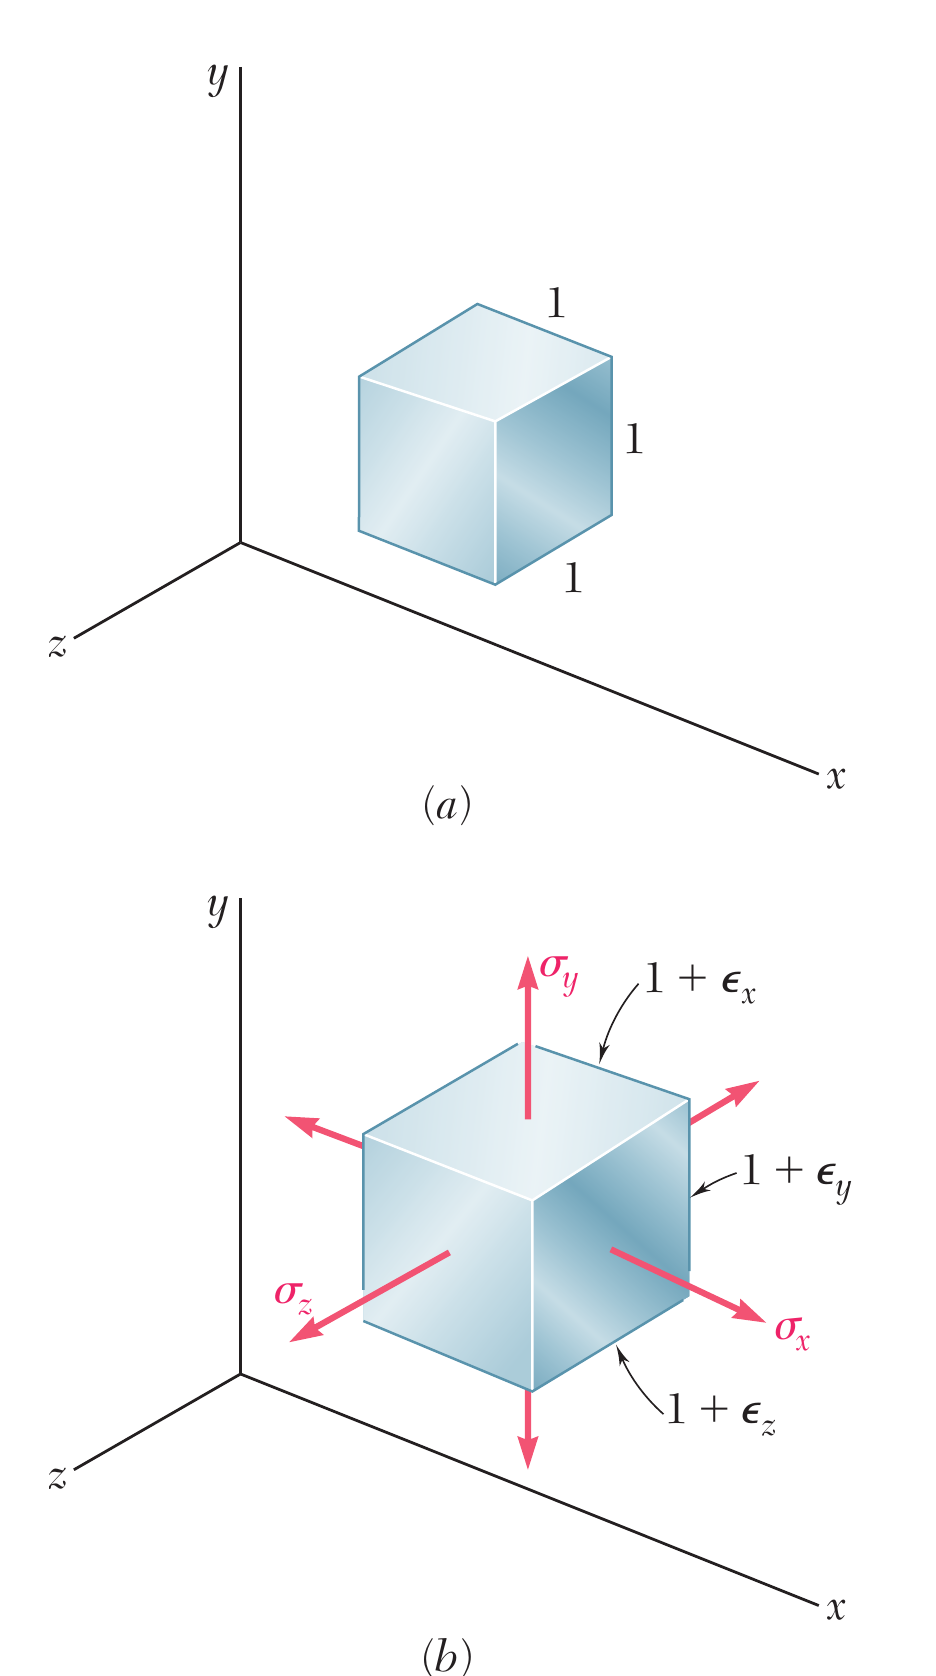
\includegraphics[width=\linewidth,height=5.5cm,keepaspectratio]{Chap_2/fig_2_39.png}
  \end{columns}
\end{frame}
% ===========
\section{Biến dạng thể tích: mô đun đàn hồi khối}
\begin{frame}[t]{Biến dạng thể tích: mô đun đàn hồi khối}
  \begin{columns}[T]
    \column{0.64\textwidth}
      \footnotesize
      \begin{itemize}
        \setlength{\itemsep}{0.4em}
        \item So với trạng thái không có ứng suất, sự thay đổi thể tích:
        \[
          e = (1+\varepsilon_x)(1+\varepsilon_y)(1+\varepsilon_z) - 1
            \approx (1 + \varepsilon_x + \varepsilon_y + \varepsilon_z) - 1
        \]
        \[
          e = \varepsilon_x + \varepsilon_y + \varepsilon_z
            = \frac{1-2\nu}{E}(\sigma_x + \sigma_y + \sigma_z)
        \]
        $e$ = biến dạng thể tích tỉ đối (độ thay đổi thể tích trên một
        đơn vị thể tích).
        \item Với phân tố chịu áp suất thủy tĩnh đều:
        \[
          e = -p\,\frac{3(1-2\nu)}{E} = -\frac{p}{k}
        \]
        \[
          k = \frac{E}{3(1-2\nu)} = \text{mô đun đàn hồi khối}
        \]
        \item Khi chịu áp suất đều, biến dạng thể tích phải âm, do đó:
        \[
          0 < \nu < \tfrac{1}{2}
        \]
      \end{itemize}
    \column{0.34\textwidth}
      \centering
      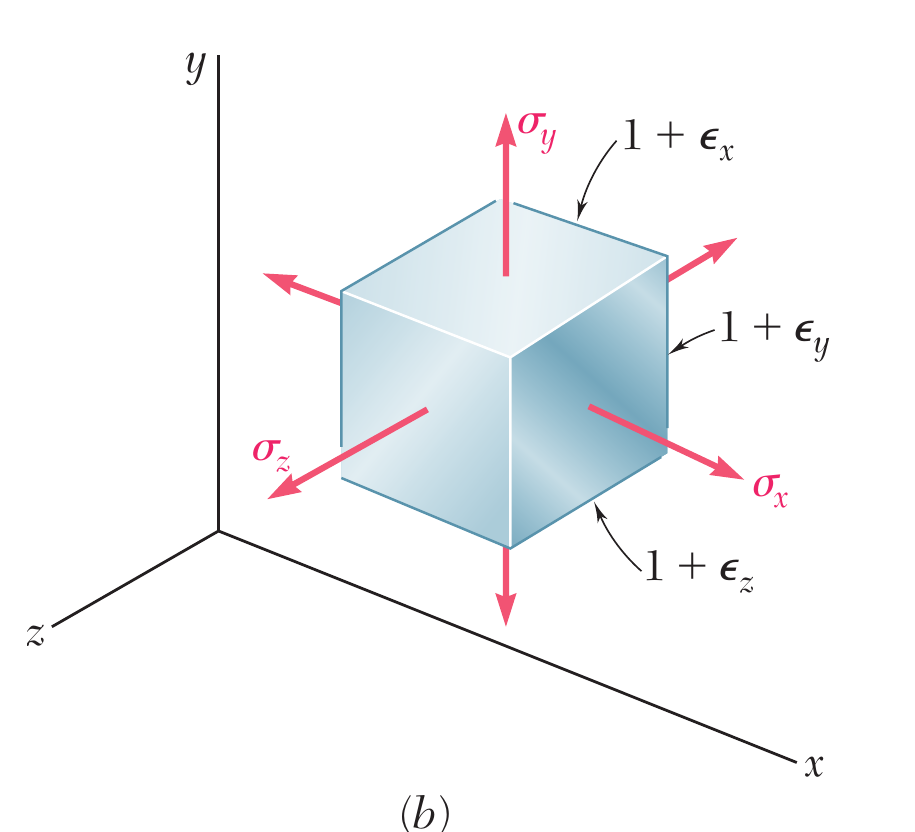
\includegraphics[width=\linewidth,height=5.5cm,keepaspectratio]{Chap_2/fig_2_39b.png}
  \end{columns}
\end{frame}
% ===========
\section{Biến dạng trượt}
\begin{frame}[t]{Biến dạng trượt}
  \begin{columns}[T]
    \column{0.36\textwidth}
      \centering
      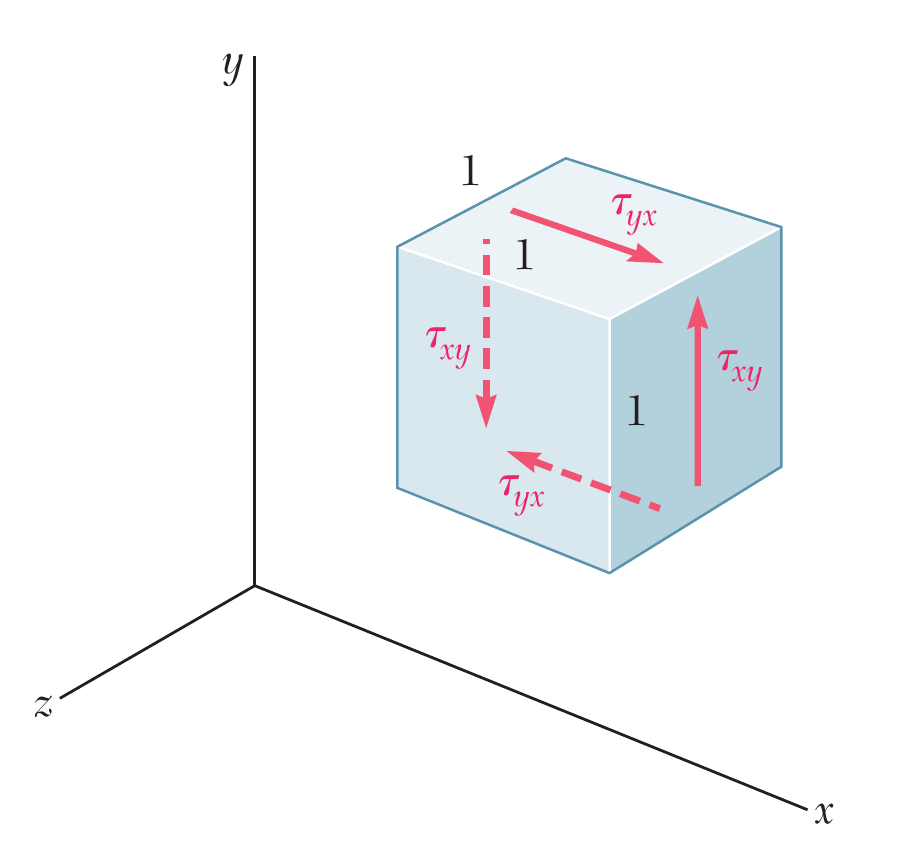
\includegraphics[width=\linewidth,height=2.9cm,keepaspectratio]{Chap_2/fig_2_42.png}\\
      \scriptsize Hình 2.42\\[2pt]
      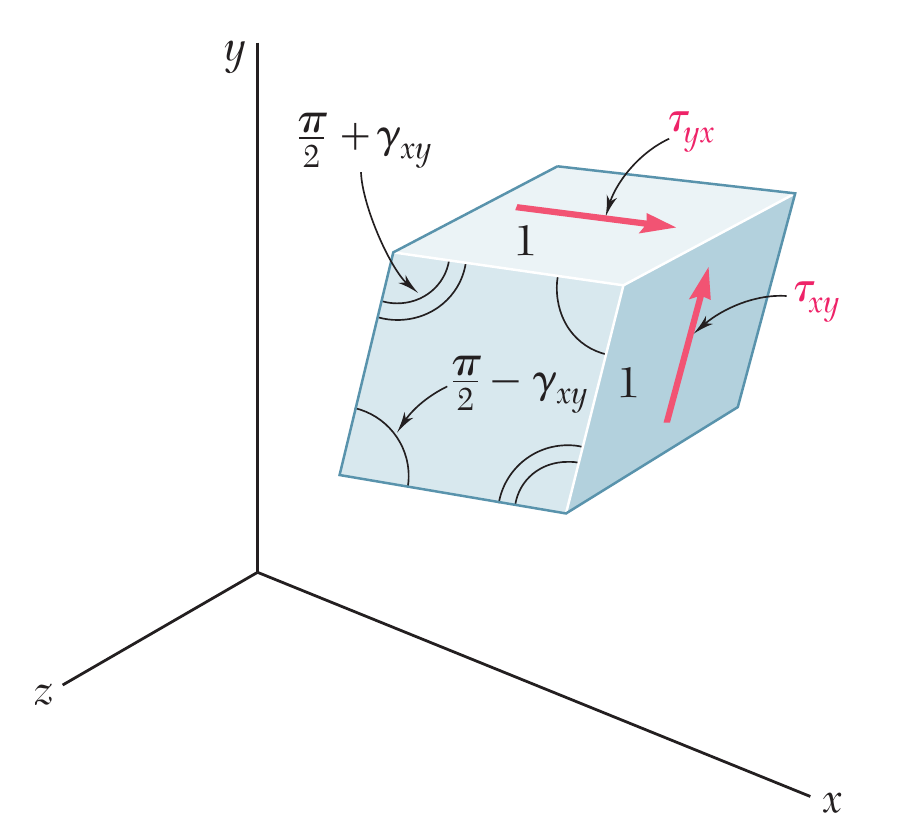
\includegraphics[width=\linewidth,height=2.6cm,keepaspectratio]{Chap_2/fig_2_43.png}\\
      \scriptsize Hình 2.43
    \column{0.62\textwidth}
      \small
      \begin{itemize}
        \setlength{\itemsep}{0.6em}
        \item Một phân tố lập phương chịu ứng suất tiếp sẽ biến dạng
              thành hình hộp xiên. Biến dạng trượt tương ứng được đo bằng
              độ thay đổi góc giữa các cạnh:
        \[
          \tau_{xy} = f(\gamma_{xy})
        \]
        \item Đồ thị ứng suất tiếp theo biến dạng trượt tương tự đồ thị
              ứng suất pháp theo biến dạng dài, chỉ khác là các giá trị
              độ bền xấp xỉ bằng một nửa. Với biến dạng nhỏ:
        \[
          \tau_{xy} = G\gamma_{xy} \quad
          \tau_{yz} = G\gamma_{yz} \quad
          \tau_{zx} = G\gamma_{zx}
        \]
        trong đó $G$ là mô đun trượt (mô đun đàn hồi trượt).
      \end{itemize}
  \end{columns}
\end{frame}
% ===========
\section{Ví dụ 2.10}
\begin{frame}[t]{Ví dụ 2.10}
  \begin{columns}[T]
    \column{0.40\textwidth}
      \centering
      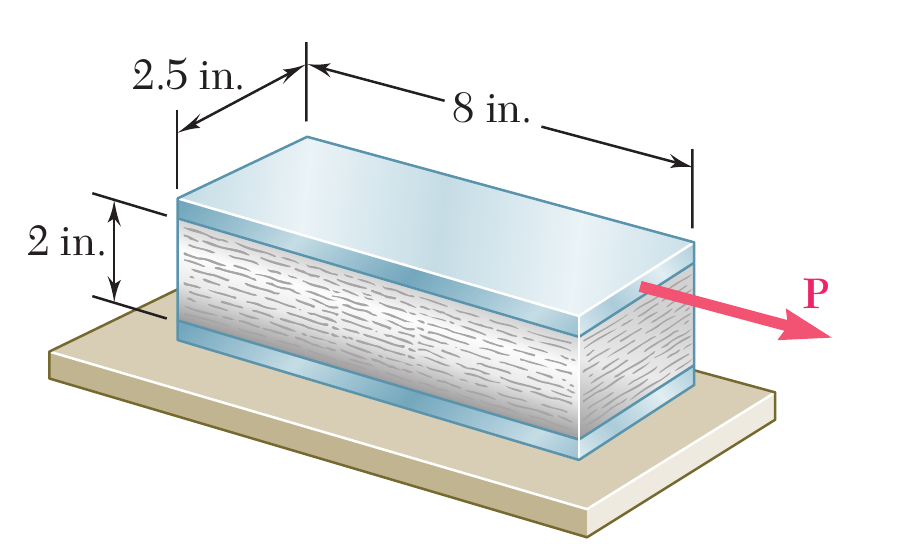
\includegraphics[width=\linewidth,height=5.5cm,keepaspectratio]{Chap_2/fig_2_47.png}
    \column{0.58\textwidth}
      \footnotesize
      Một khối vật liệu hình hộp chữ nhật có mô đun trượt
      $G = 630\,\mathrm{MPa}$ được dán vào hai tấm cứng nằm ngang. Tấm
      dưới cố định, tấm trên chịu lực ngang $P$. Biết tấm trên dịch
      chuyển 1,0 mm dưới tác dụng của lực, xác định a) biến dạng trượt
      trung bình trong vật liệu, và b) lực $P$ tác dụng lên tấm.

      \vspace{0.5em}
      \textbf{LỜI GIẢI:}
      \begin{itemize}
        \setlength{\itemsep}{0.4em}
        \item Xác định biến dạng góc trung bình, hay biến dạng trượt,
              của khối.
        \item Áp dụng định luật Hooke cho ứng suất tiếp và biến dạng
              trượt để tìm ứng suất tiếp tương ứng.
        \item Dùng định nghĩa ứng suất tiếp để tìm lực $P$.
      \end{itemize}
  \end{columns}
\end{frame}
% ===========
\begin{frame}[t]{Ví dụ 2.10 (tiếp)}
  \begin{columns}[T]
    \column{0.36\textwidth}
      \centering
      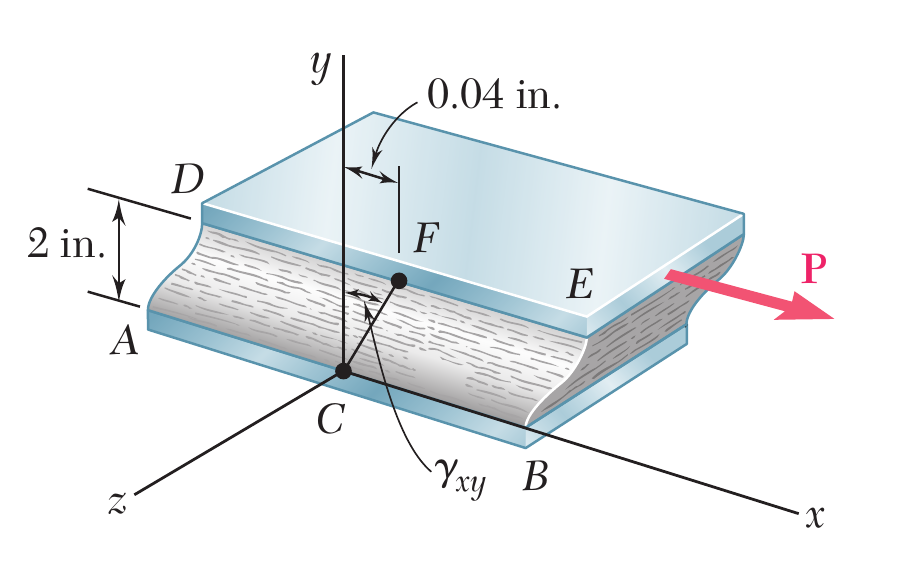
\includegraphics[width=\linewidth,height=5.5cm,keepaspectratio]{Chap_2/fig_2_48.png}
    \column{0.62\textwidth}
      \small
      \begin{itemize}
        \setlength{\itemsep}{0.7em}
        \item Xác định biến dạng góc trung bình, hay biến dạng trượt,
              của khối:
        \[
          \gamma_{xy} \approx \tan\gamma_{xy}
            = \frac{1\,\mathrm{mm}}{50\,\mathrm{mm}}
          \qquad \gamma_{xy} = 0{,}020\,\mathrm{rad}
        \]
        \item Áp dụng định luật Hooke để tìm ứng suất tiếp tương ứng:
        \[
          \tau_{xy} = G\gamma_{xy} = (630\,\mathrm{MPa})(0{,}020\,\mathrm{rad})
            = 12{,}6\,\mathrm{MPa}
        \]
        \item Dùng định nghĩa ứng suất tiếp để tìm lực $P$:
        \[
          P = \tau_{xy}A = (12{,}6\times10^{6})(0{,}2)(0{,}062)
            = 156{,}2\times10^{3}\,\mathrm{N}
        \]
        \[
          \boxed{P = 156{,}2\,\mathrm{kN}}
        \]
      \end{itemize}
  \end{columns}
\end{frame}
% ===========
\section{Quan hệ giữa \texorpdfstring{$E$, $\nu$ và $G$}{E, nu và G}}
\begin{frame}[t]{Quan hệ giữa $E$, $\nu$ và $G$}
  \begin{columns}[T]
    \column{0.60\textwidth}
      \small
      \begin{itemize}
        \setlength{\itemsep}{0.6em}
        \item Một thanh mảnh chịu tải trọng dọc trục sẽ giãn dài theo
              phương dọc trục và co lại theo phương ngang.
        \item Một phân tố ban đầu là hình lập phương, đặt như hình trên,
              sẽ biến dạng thành hình hộp chữ nhật. Tải trọng dọc trục
              gây ra biến dạng dài.
        \item Nếu phân tố lập phương được đặt như hình dưới, nó sẽ biến
              dạng thành hình thoi. Tải trọng dọc trục cũng gây ra biến
              dạng trượt.
        \item Các thành phần biến dạng dài và biến dạng trượt có quan hệ:
        \[
          \frac{E}{2G} = (1 + \nu)
        \]
      \end{itemize}
    \column{0.38\textwidth}
      \centering
      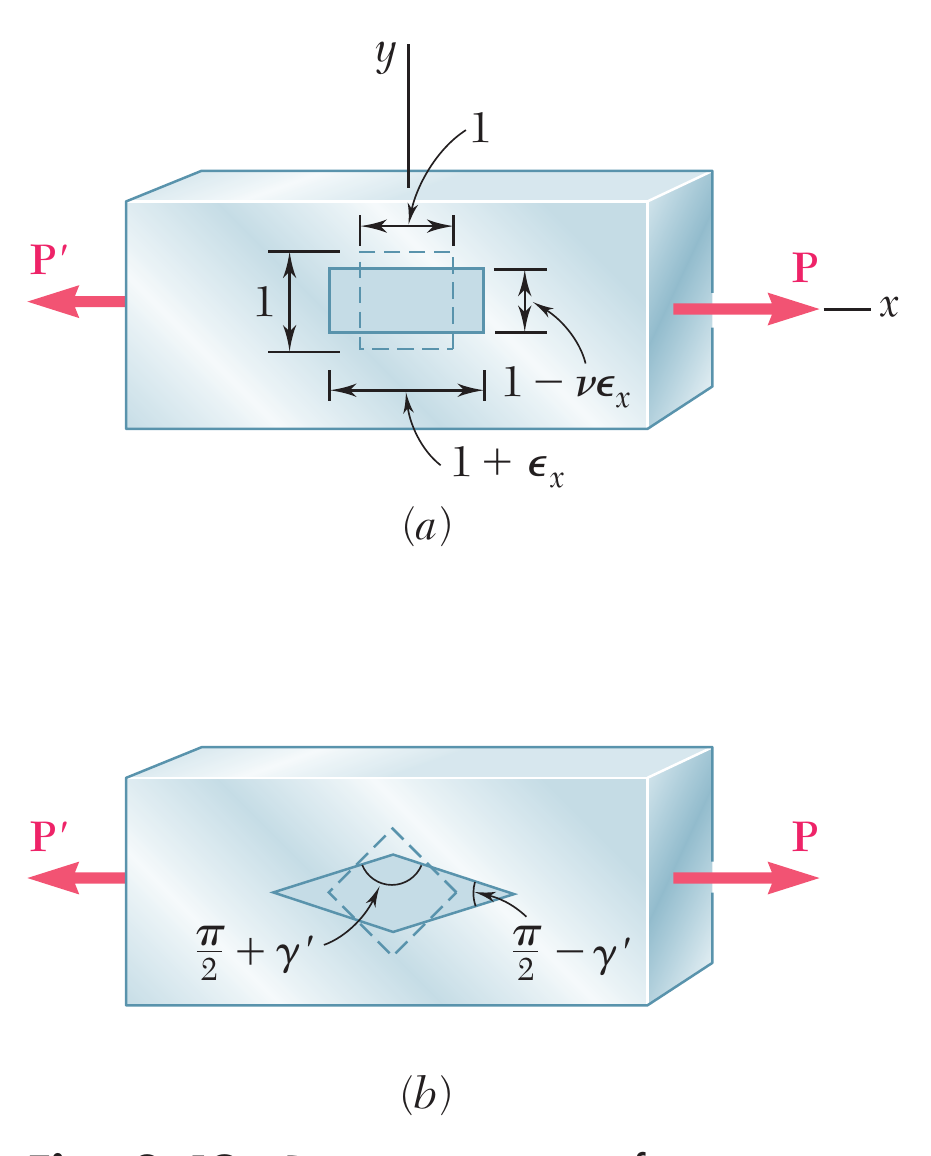
\includegraphics[width=\linewidth,height=5.5cm,keepaspectratio]{Chap_2/fig_2_49.png}
  \end{columns}
\end{frame}
% ===========
\section{Bài mẫu 2.5}
\begin{frame}[t]{Bài mẫu 2.5}
  \begin{columns}[T]
    \column{0.40\textwidth}
      \centering
      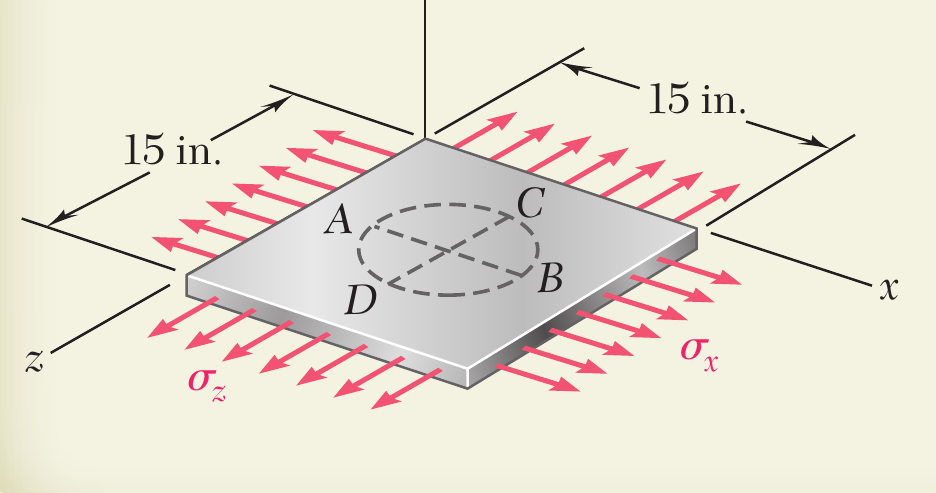
\includegraphics[width=\linewidth,height=5.5cm,keepaspectratio]{Chap_2/sp_2_5_1.png}
    \column{0.58\textwidth}
      \small
      Một đường tròn đường kính $d = 225\,\mathrm{mm}$ được vạch trên một
      tấm nhôm chưa chịu lực, chiều dày $t = 18\,\mathrm{mm}$. Sau đó các
      lực tác dụng trong mặt phẳng tấm gây ra các ứng suất pháp
      $\sigma_x = 84\,\mathrm{MPa}$ và $\sigma_z = 140\,\mathrm{MPa}$.

      \vspace{0.5em}
      Với $E = 70\,\mathrm{GPa}$ và $\nu = 1/3$, xác định độ thay đổi của:
      \begin{enumerate}[a)]
        \item chiều dài đường kính $AB$,
        \item chiều dài đường kính $CD$,
        \item chiều dày tấm, và
        \item thể tích tấm.
      \end{enumerate}
  \end{columns}
\end{frame}
% ===========
\begin{frame}[t]{Bài mẫu 2.5 (tiếp)}
  \begin{columns}[T]
    \column{0.50\textwidth}
      \footnotesize
      \textbf{LỜI GIẢI:}
      \begin{itemize}
        \item Áp dụng định luật Hooke tổng quát để tìm ba thành phần
              biến dạng dài:
      \end{itemize}
      \[
        \begin{aligned}
          \varepsilon_x &= +\frac{\sigma_x}{E} - \frac{\nu\sigma_y}{E}
                           - \frac{\nu\sigma_z}{E}\\
            &= \frac{1}{70\times10^{3}\,\mathrm{MPa}}
               \left[(84\,\mathrm{MPa}) - 0 - \tfrac{1}{3}(140\,\mathrm{MPa})\right]\\
            &= +0{,}533\times10^{-3}\,\mathrm{mm/mm}\\[0.3em]
          \varepsilon_y &= -\frac{\nu\sigma_x}{E} + \frac{\sigma_y}{E}
                           - \frac{\nu\sigma_z}{E}
             = -1{,}067\times10^{-3}\,\mathrm{mm/mm}\\[0.3em]
          \varepsilon_z &= -\frac{\nu\sigma_x}{E} - \frac{\nu\sigma_y}{E}
                           + \frac{\sigma_z}{E}
             = +1{,}600\times10^{-3}\,\mathrm{mm/mm}
        \end{aligned}
      \]
    \column{0.48\textwidth}
      \footnotesize
      \begin{itemize}
        \setlength{\itemsep}{0.5em}
        \item Tính các thành phần biến dạng:
        \[
          \delta_{B/A} = \varepsilon_x d
            = (+0{,}533\times10^{-3})(225\,\mathrm{mm})
        \]
        \[ \boxed{\delta_{B/A} = +0{,}12\,\mathrm{mm}} \]
        \[
          \delta_{C/D} = \varepsilon_z d
            = (+1{,}600\times10^{-3})(225\,\mathrm{mm})
        \]
        \[ \boxed{\delta_{C/D} = +0{,}36\,\mathrm{mm}} \]
        \[
          \delta_t = \varepsilon_y t = (-1{,}067\times10^{-3})(18\,\mathrm{mm})
        \]
        \[ \boxed{\delta_t = -0{,}0192\,\mathrm{mm}} \]
        \item Tìm độ thay đổi thể tích:
        \[
          e = \varepsilon_x + \varepsilon_y + \varepsilon_z
            = 1{,}067\times10^{-3}\,\mathrm{mm^3/mm^3}
        \]
        \[
          \Delta V = eV = 1{,}067\times10^{-3}(380\times380\times18)\,\mathrm{mm}^3
        \]
        \[ \boxed{\Delta V = +2733\,\mathrm{mm}^3} \]
      \end{itemize}
  \end{columns}
\end{frame}
% ===========
\section{Vật liệu composite}
\begin{frame}[t]{Vật liệu composite}
  \begin{columns}[T]
    \column{0.60\textwidth}
      \small
      \begin{itemize}
        \setlength{\itemsep}{0.5em}
        \item Vật liệu composite cốt sợi được tạo thành từ các lớp sợi
              graphit, thủy tinh hoặc polyme nằm trong nền nhựa.
        \item Ứng suất pháp và biến dạng dài liên hệ với nhau theo định
              luật Hooke nhưng với mô đun đàn hồi phụ thuộc phương:
        \[
          E_x = \frac{\sigma_x}{\varepsilon_x} \qquad
          E_y = \frac{\sigma_y}{\varepsilon_y} \qquad
          E_z = \frac{\sigma_z}{\varepsilon_z}
        \]
        \item Biến dạng co ngang liên hệ qua hệ số Poisson phụ thuộc
              phương, ví dụ:
        \[
          \nu_{xy} = -\frac{\varepsilon_y}{\varepsilon_x} \qquad
          \nu_{xz} = -\frac{\varepsilon_z}{\varepsilon_x}
        \]
        \item Vật liệu có cơ tính phụ thuộc phương được gọi là vật liệu
              \emph{dị hướng}.
      \end{itemize}
    \column{0.38\textwidth}
      \centering
      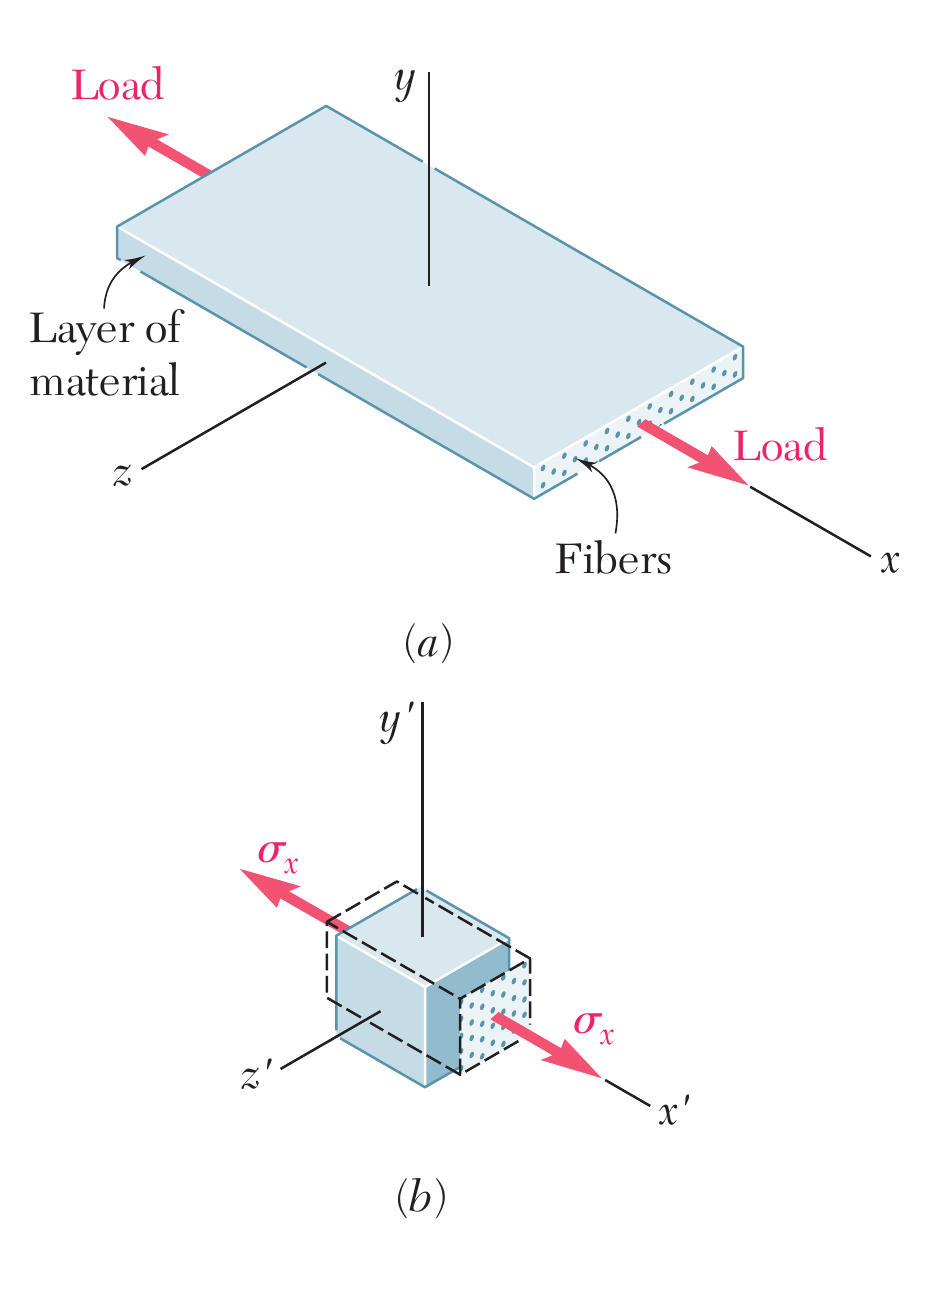
\includegraphics[width=\linewidth,height=7cm,keepaspectratio]{Chap_2/fig_2_51.png}
  \end{columns}
\end{frame}
% ===========
\section{Nguyên lý Saint-Venant}
\begin{frame}[t]{Nguyên lý Saint-Venant}
  \begin{columns}[T]
    \column{0.40\textwidth}
      \centering
      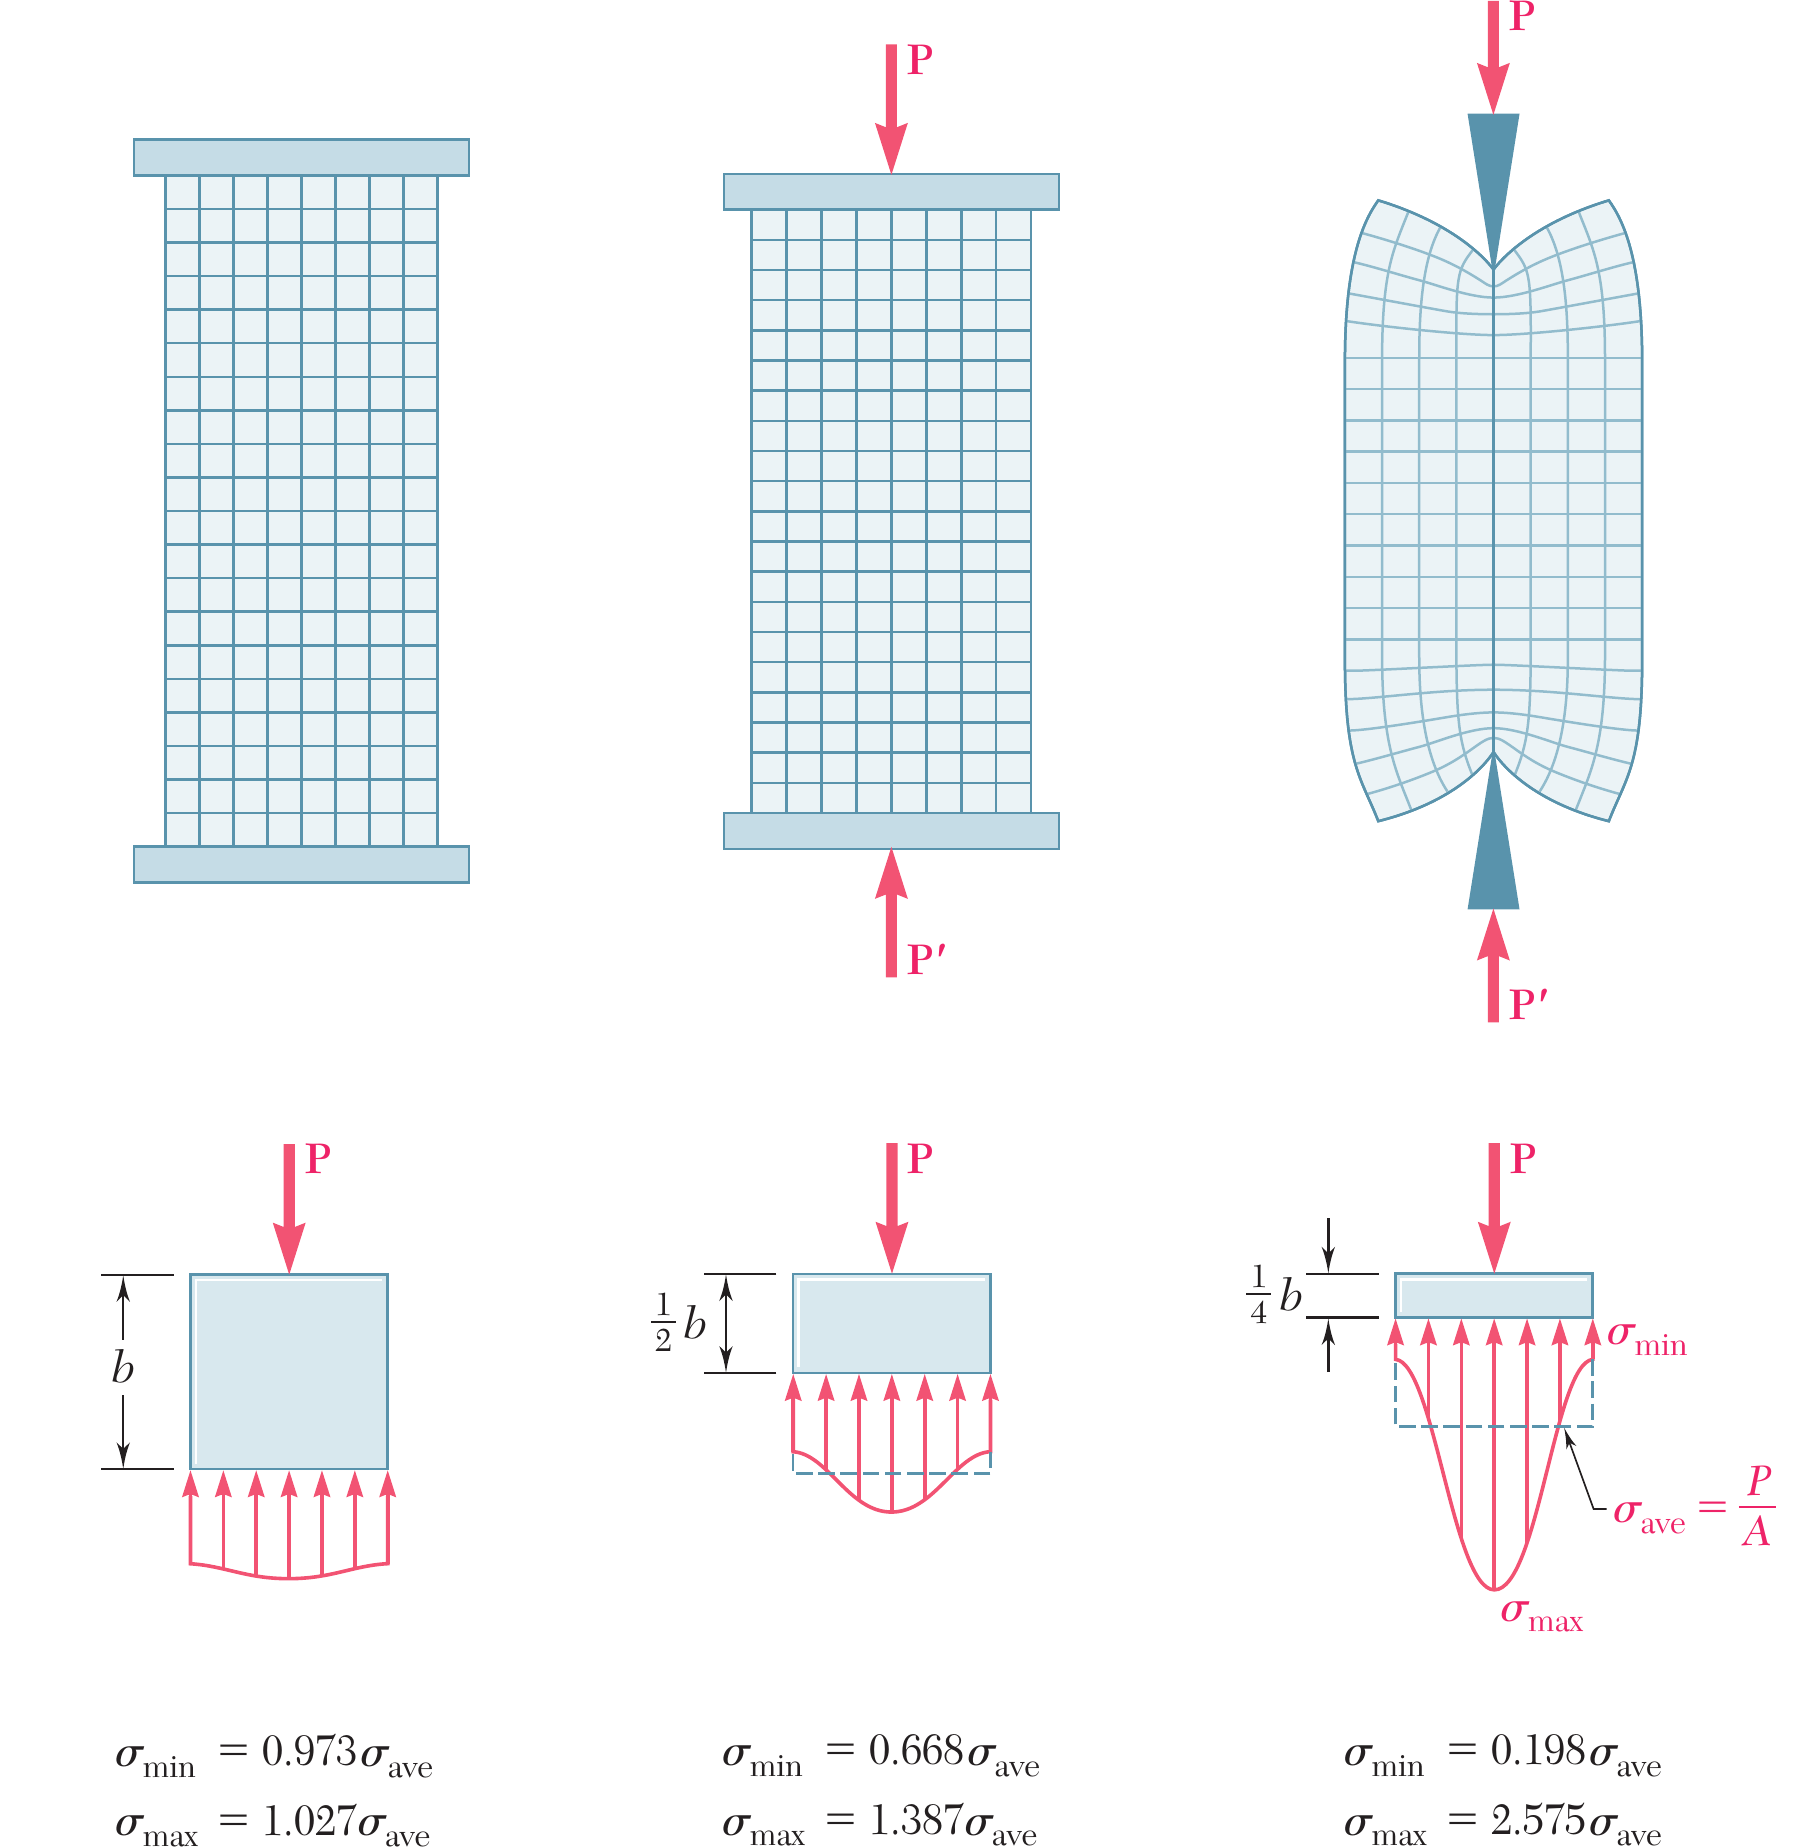
\includegraphics[width=\linewidth,height=8cm,keepaspectratio]{Chap_2/fig_2_55_57.png}\\[2pt]
    \column{0.58\textwidth}
      \small
      \begin{itemize}
        \setlength{\itemsep}{0.6em}
        \item Tải trọng truyền qua các tấm cứng tạo ra phân bố ứng suất
              và biến dạng đều.
        \item Tải trọng tập trung gây ra ứng suất lớn trong vùng lân cận
              điểm đặt lực.
        \item Phân bố ứng suất và biến dạng trở nên đều ở khoảng cách
              tương đối ngắn tính từ điểm đặt lực.
        \item \textbf{Nguyên lý Saint-Venant:} Có thể giả thiết phân bố
              ứng suất không phụ thuộc vào cách đặt tải, trừ vùng lân
              cận ngay sát điểm đặt lực.
      \end{itemize}
  \end{columns}
\end{frame}
% ===========
\section{Tập trung ứng suất: lỗ khoét}
\begin{frame}[t]{Tập trung ứng suất: lỗ khoét}
  \begin{columns}[T]
    \column{0.40\textwidth}
      \centering
      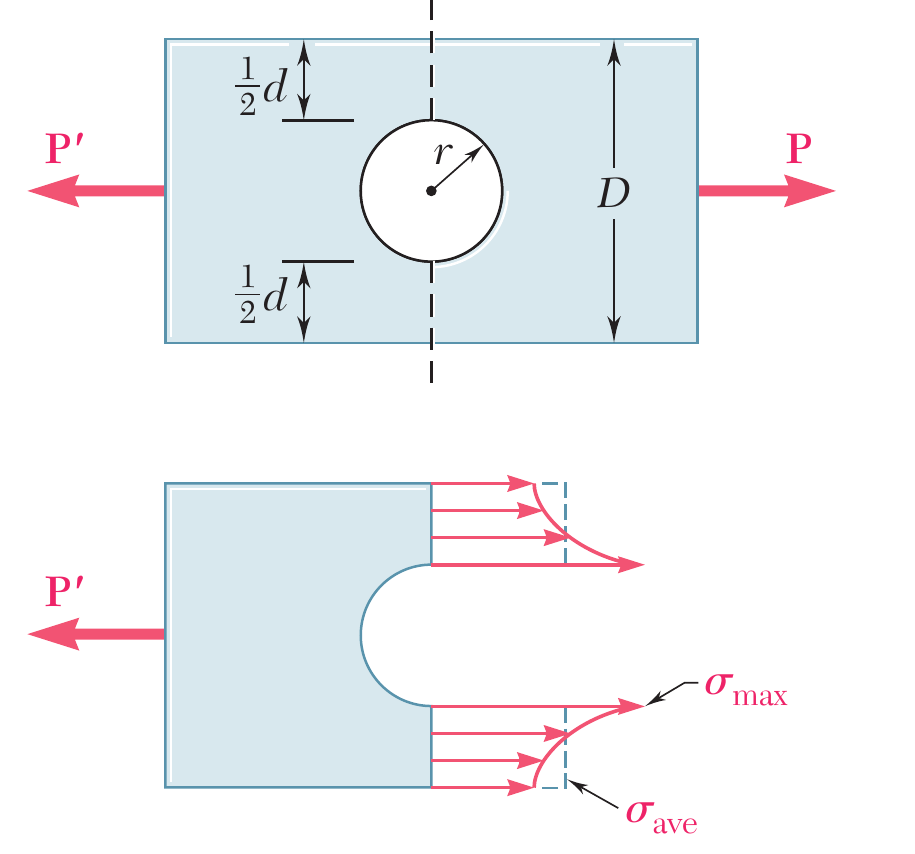
\includegraphics[width=\linewidth,height=3cm,keepaspectratio]{Chap_2/fig_2_58.png}
      \small
      \vspace{0.5em}

      Sự thay đổi đột ngột của mặt cắt ngang có thể gây ra ứng suất cục
      bộ lớn, hay ứng suất tập trung.
      \[
        K = \frac{\sigma_{\max}}{\sigma_{\mathrm{tb}}}
      \]
    \column{0.58\textwidth}
      \centering
      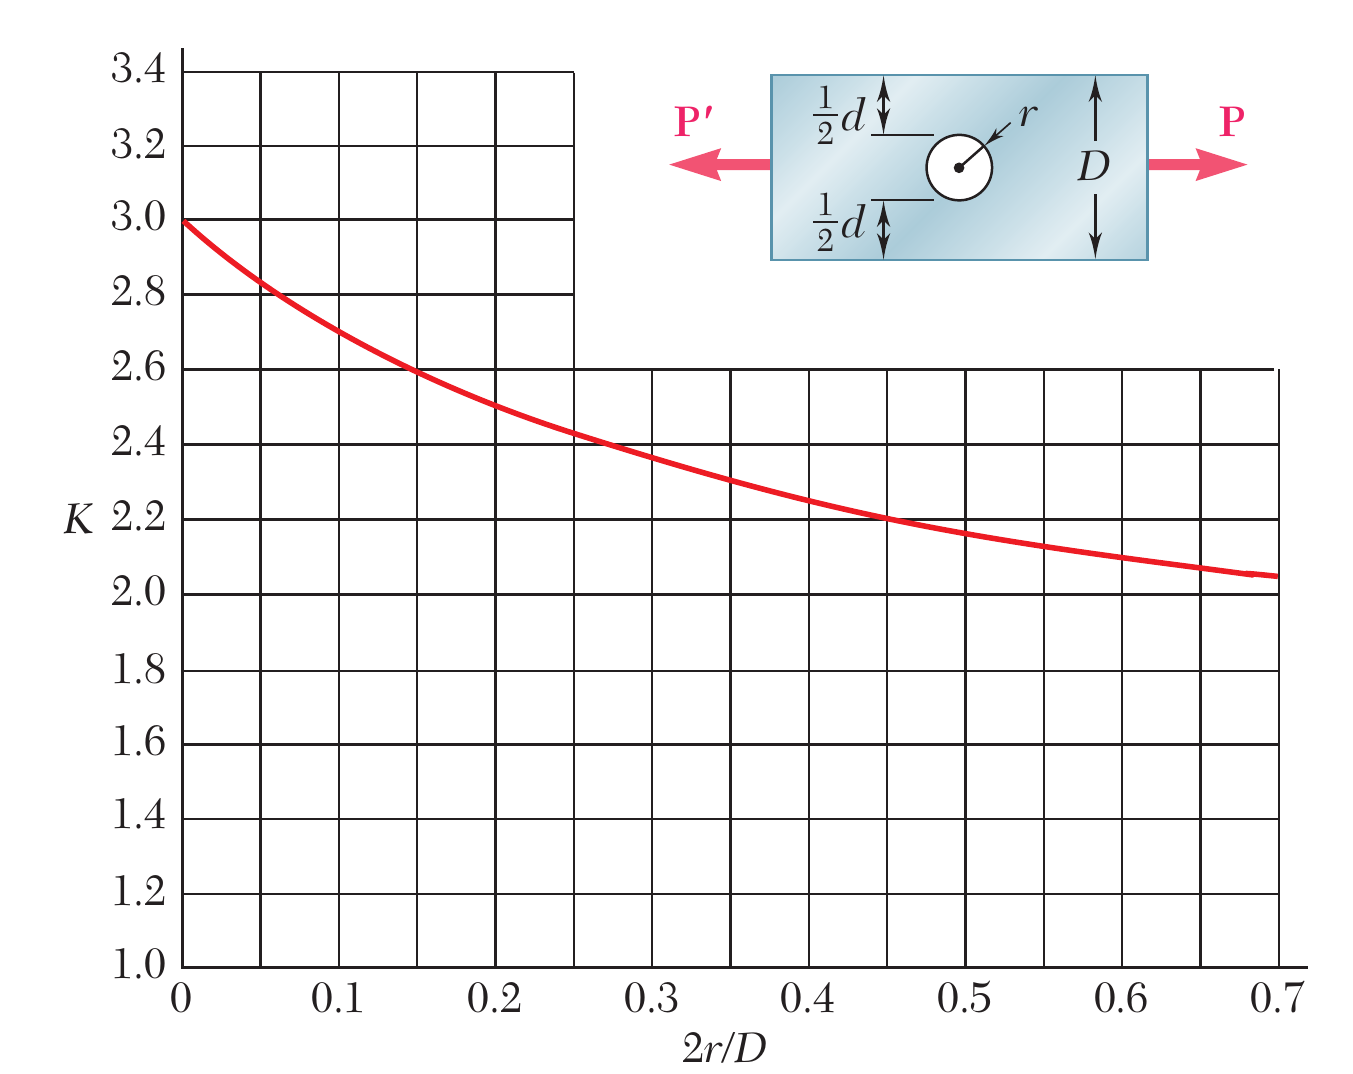
\includegraphics[width=\linewidth,height=5.5cm,keepaspectratio]{Chap_2/fig_2_60a.png}\\
      \scriptsize (a) Thanh dẹt có lỗ khoét
  \end{columns}
\end{frame}
% ===========
\section{Tập trung ứng suất: góc lượn}
\begin{frame}[t]{Tập trung ứng suất: góc lượn}
  \begin{columns}[T]
    \column{0.40\textwidth}
      \centering
      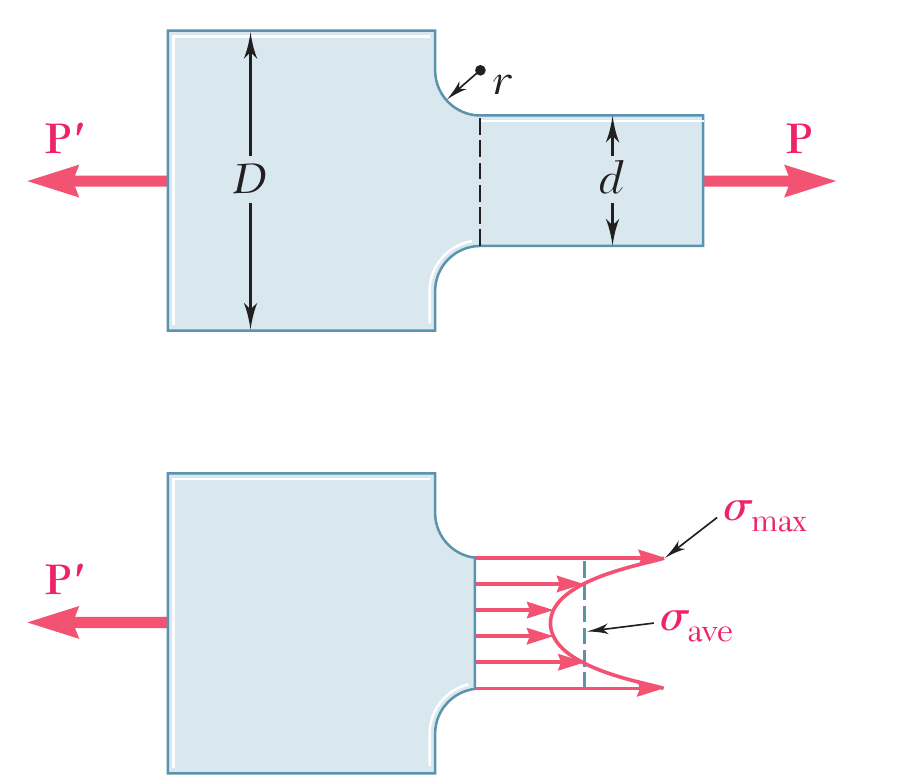
\includegraphics[width=\linewidth,height=5.5cm,keepaspectratio]{Chap_2/fig_2_59.png}
    \column{0.58\textwidth}
      \centering
      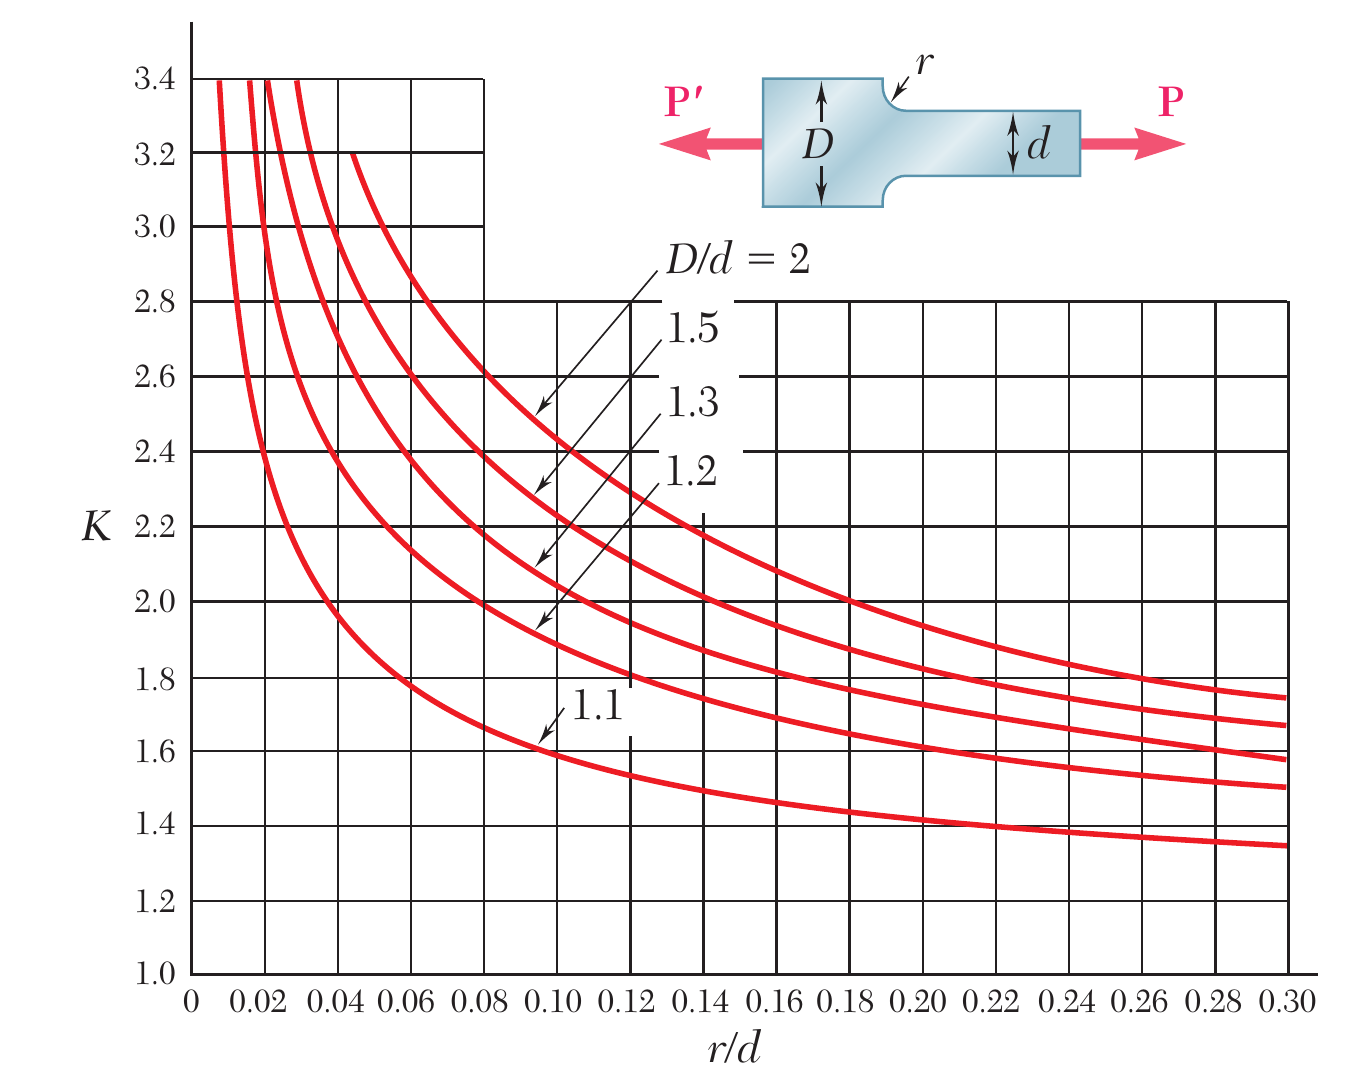
\includegraphics[width=\linewidth,height=5.5cm,keepaspectratio]{Chap_2/fig_2_60b.png}\\
      \scriptsize (b) Thanh dẹt có góc lượn
  \end{columns}
\end{frame}
% ===========
\section{Ví dụ 2.12}
\begin{frame}[t]{Ví dụ 2.12}
  \begin{columns}[T]
    \column{0.40\textwidth}
      \centering
      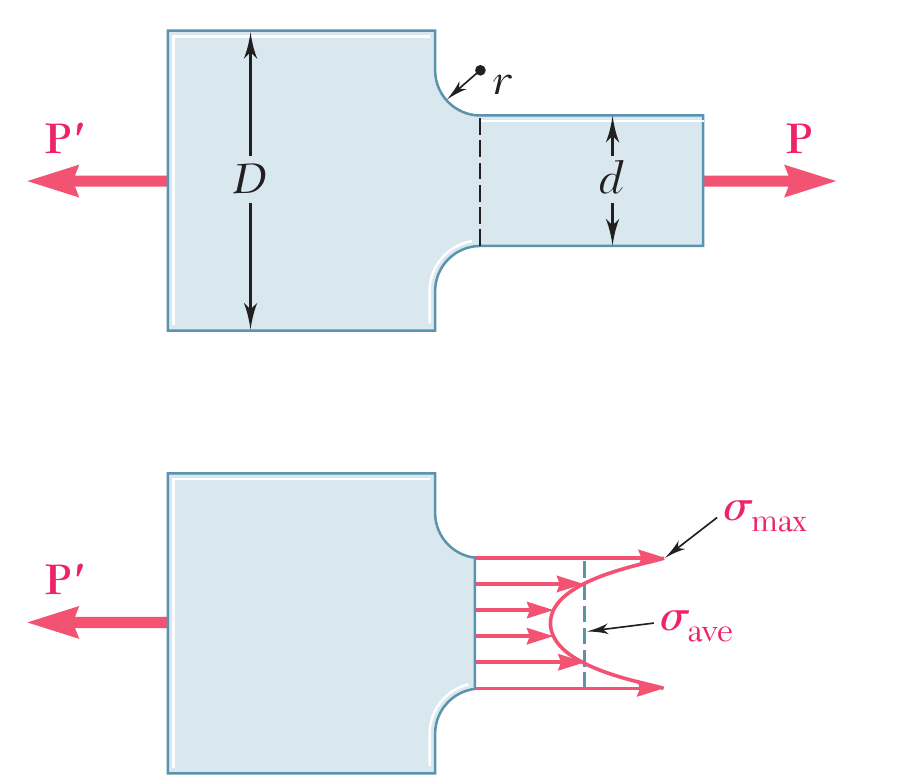
\includegraphics[width=\linewidth,height=5.5cm,keepaspectratio]{Chap_2/fig_2_59.png}
    \column{0.58\textwidth}
      \small
      Xác định tải trọng dọc trục lớn nhất $P$ mà một thanh thép dẹt có
      thể chịu được an toàn. Thanh gồm hai đoạn, cùng dày 10 mm, rộng lần
      lượt 40 mm và 60 mm, nối với nhau bằng góc lượn bán kính
      $r = 8\,\mathrm{mm}$. Giả thiết ứng suất pháp cho phép là
      165 MPa.

      \vspace{0.5em}
      \textbf{LỜI GIẢI:}
      \begin{itemize}
        \setlength{\itemsep}{0.4em}
        \item Xác định các tỉ số hình học và tra hệ số tập trung ứng
              suất từ Hình 2.60b.
        \item Tìm ứng suất pháp trung bình cho phép từ ứng suất cho phép
              của vật liệu và hệ số tập trung ứng suất.
        \item Áp dụng định nghĩa ứng suất pháp để tìm tải trọng cho phép.
      \end{itemize}
  \end{columns}
\end{frame}
% ===========
\begin{frame}[t]{Ví dụ 2.12 (tiếp)}
  \begin{columns}[T]
    \column{0.58\textwidth}
      \small
      \begin{itemize}
        \setlength{\itemsep}{0.5em}
        \item Xác định các tỉ số hình học và tra hệ số tập trung ứng
              suất từ Hình 2.60b:
        \[
          \frac{D}{d} = \frac{60\,\mathrm{mm}}{40\,\mathrm{mm}} = 1{,}50
          \qquad
          \frac{r}{d} = \frac{8\,\mathrm{mm}}{40\,\mathrm{mm}} = 0{,}20
        \]
        \[
          K = 1{,}82
        \]
        \item Tìm ứng suất pháp trung bình cho phép:
        \[
          \sigma_{\mathrm{tb}} = \frac{\sigma_{\max}}{K}
            = \frac{165\,\mathrm{MPa}}{1{,}82} = 90{,}7\,\mathrm{MPa}
        \]
        \item Áp dụng định nghĩa ứng suất pháp để tìm tải trọng cho phép:
        \[
          P = A\sigma_{\mathrm{tb}} = (40)(10)(90{,}7)
            = 36{,}3\times10^{3}\,\mathrm{N}
        \]
        \[
          \boxed{P = 36{,}3\,\mathrm{kN}}
        \]
      \end{itemize}
    \column{0.40\textwidth}
      \centering
      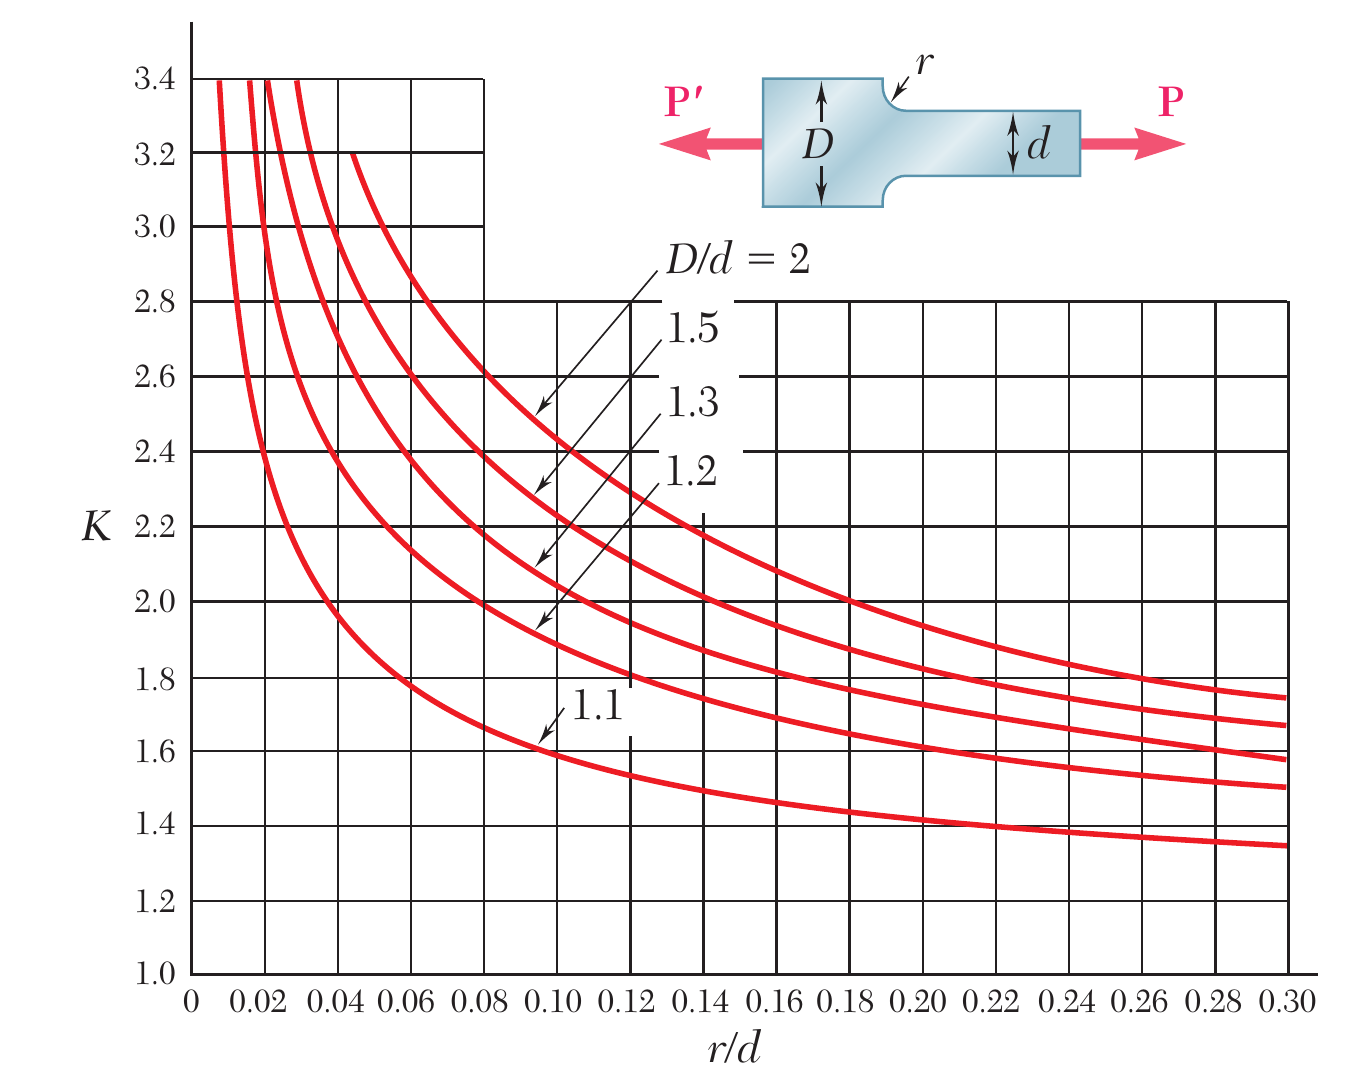
\includegraphics[width=\linewidth,height=5.5cm,keepaspectratio]{Chap_2/fig_2_60b.png}\\
      \tiny (b) Thanh dẹt có góc lượn
  \end{columns}
\end{frame}
% ===========
\section{Vật liệu đàn -- dẻo}
\begin{frame}[t]{Vật liệu đàn -- dẻo}
  \begin{columns}[T]
    \column{0.60\textwidth}
      \small
      \begin{itemize}
        \setlength{\itemsep}{0.35em}
        \item Các phân tích trước đây dựa trên giả thiết quan hệ ứng suất
              -- biến dạng tuyến tính, tức là ứng suất nhỏ hơn giới hạn
              chảy.
        \item Giả thiết này phù hợp với vật liệu giòn, bị phá hủy mà không
              chảy dẻo.
        \item Nếu ứng suất vượt quá giới hạn chảy của vật liệu dẻo thì
              xuất hiện biến dạng dẻo.
        \item Việc phân tích biến dạng dẻo được đơn giản hóa bằng cách giả
              thiết vật liệu đàn -- dẻo lý tưởng.
        \item Biến dạng của vật liệu đàn -- dẻo được chia thành miền đàn
              hồi và miền dẻo.
        \item Biến dạng dư (vĩnh viễn) xuất hiện khi chất tải vượt quá
              giới hạn chảy.
      \end{itemize}
    \column{0.38\textwidth}
      \centering
      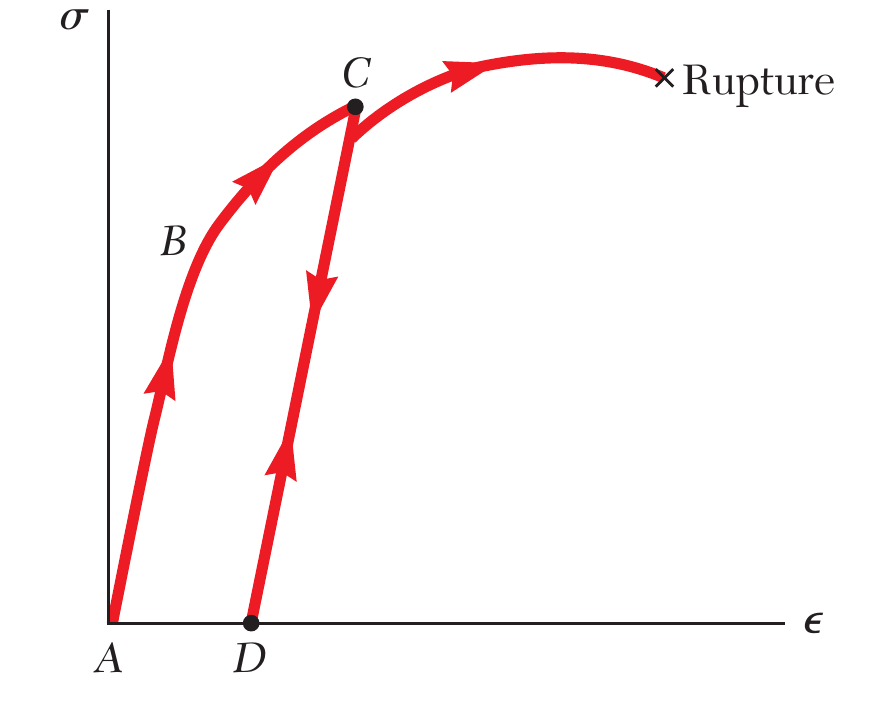
\includegraphics[width=\linewidth,height=2.9cm,keepaspectratio]{Chap_2/fig_2_14.png}\\[2pt]
      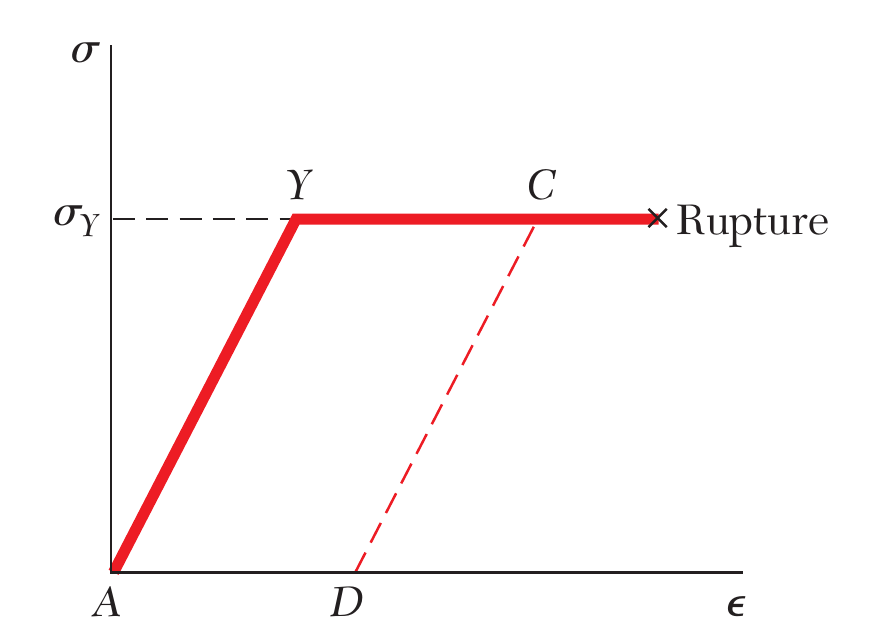
\includegraphics[width=\linewidth,height=2.9cm,keepaspectratio]{Chap_2/fig_2_61.png}
  \end{columns}
\end{frame}
% ===========
\section{Biến dạng dẻo}
\begin{frame}[t]{Biến dạng dẻo}
  \begin{columns}[T]
    \column{0.60\textwidth}
      \small
      \begin{itemize}
        \setlength{\itemsep}{0.4em}
        \item Biến dạng đàn hồi khi ứng suất lớn nhất còn nhỏ hơn giới
              hạn chảy:
        \[
          P = \sigma_{\mathrm{tb}}A = \frac{\sigma_{\max}A}{K}
        \]
        \item Ứng suất lớn nhất bằng giới hạn chảy tại tải trọng đàn hồi
              lớn nhất:
        \[
          P_Y = \frac{\sigma_Y A}{K}
        \]
        \item Khi tải trọng vượt quá tải trọng đàn hồi lớn nhất, một vùng
              biến dạng dẻo hình thành gần lỗ khoét.
        \item Khi tải trọng tăng, vùng dẻo mở rộng cho đến khi toàn bộ mặt
              cắt có ứng suất đều bằng giới hạn chảy:
        \[
          P_U = \sigma_Y A = K P_Y
        \]
      \end{itemize}
    \column{0.38\textwidth}
      \centering
      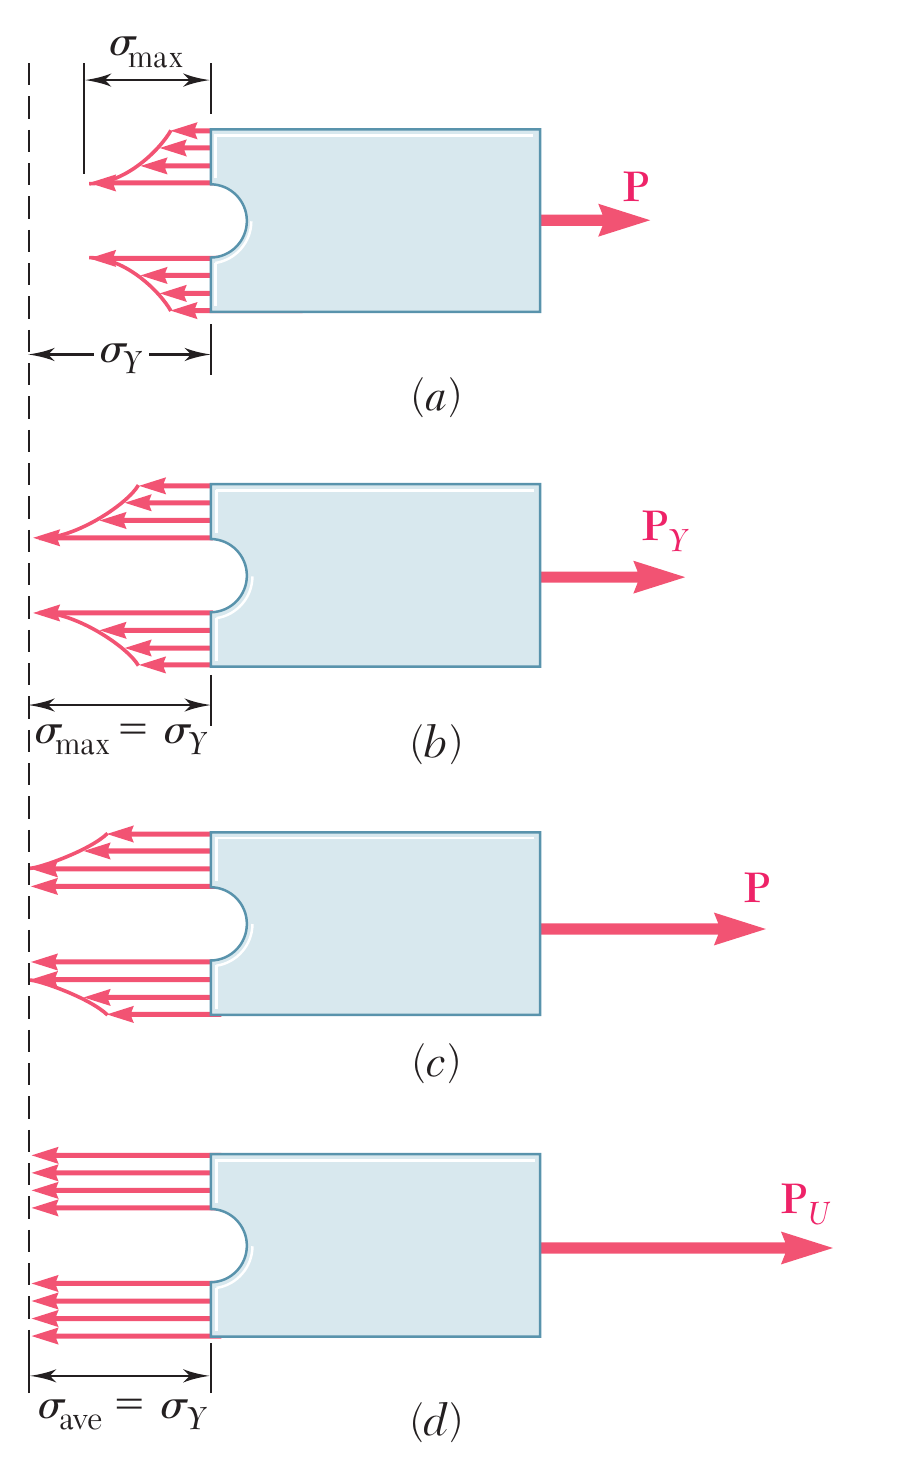
\includegraphics[width=\linewidth,height=7cm,keepaspectratio]{Chap_2/fig_2_65.png}
  \end{columns}
\end{frame}
% ===========
\section{Ứng suất dư}
\begin{frame}[t]{Ứng suất dư}
  \small
  \begin{itemize}
    \setlength{\itemsep}{0.9em}
    \item Khi một cấu kiện đơn lẻ được chất tải đều vượt quá giới hạn
          chảy rồi dỡ tải, nó bị biến dạng vĩnh viễn nhưng mọi ứng suất
          đều biến mất. Đây không phải là kết quả tổng quát.
    \item Ứng suất dư sẽ còn lại trong kết cấu sau khi chất tải và dỡ
          tải nếu:
          \begin{itemize}
            \item chỉ một phần của kết cấu bị biến dạng dẻo
            \item các phần khác nhau của kết cấu có biến dạng dẻo khác nhau
          \end{itemize}
    \item Ứng suất dư cũng xuất hiện do kết cấu hoặc cấu kiện bị nung
          nóng hoặc làm nguội không đều.
  \end{itemize}
\end{frame}
% ===========
\section{Ví dụ 2.14, 2.15, 2.16}
\begin{frame}[t]{Ví dụ 2.14, 2.15, 2.16}
  \begin{columns}[T]
    \column{0.40\textwidth}
      \centering
      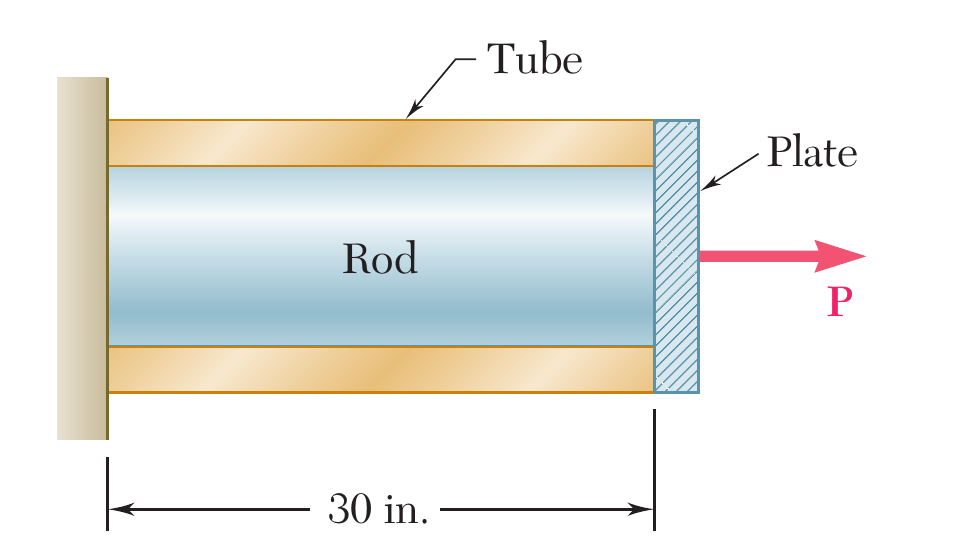
\includegraphics[width=\linewidth,height=5.5cm,keepaspectratio]{Chap_2/fig_2_62.png}
    \column{0.58\textwidth}
      \small
      Một thanh trụ tròn đặt bên trong một ống có cùng chiều dài. Hai đầu
      thanh và ống được gắn vào một gối cứng ở một phía và một tấm cứng ở
      phía kia. Tải trọng tác dụng lên cụm thanh -- ống tăng từ 0 đến
      25 kN rồi giảm về 0.
      \begin{enumerate}[a)]
        \setlength{\itemsep}{0.3em}
        \item vẽ biểu đồ tải trọng -- chuyển vị của cụm thanh -- ống
        \item xác định độ giãn dài lớn nhất
        \item xác định biến dạng dư
        \item tính ứng suất dư trong thanh và trong ống.
      \end{enumerate}
      \vspace{0.3em}
      \footnotesize
      $A_r = 48\,\mathrm{mm}^2$, $E_r = 210\,\mathrm{GPa}$,
      $(\sigma_r)_Y = 250\,\mathrm{MPa}$\\
      $A_t = 62\,\mathrm{mm}^2$, $E_t = 105\,\mathrm{GPa}$,
      $(\sigma_t)_Y = 310\,\mathrm{MPa}$, $L = 750\,\mathrm{mm}$
  \end{columns}
\end{frame}
% ===========
\begin{frame}[t]{Ví dụ 2.14, 2.15, 2.16 (tiếp)}
  \begin{columns}[T]
    \column{0.60\textwidth}
      \footnotesize
      a) Vẽ biểu đồ tải trọng -- chuyển vị của cụm thanh -- ống:
      \[
        (P_r)_Y = (\sigma_r)_Y A_r = (250\times10^{6}\,\mathrm{Pa})
                  (48\times10^{-6}\,\mathrm{m}^2) = 12\,\mathrm{kN}
      \]
      \[
        (\delta_r)_Y = (\varepsilon_r)_Y L = \frac{(\sigma_r)_Y}{E_r}L
          = \frac{250\times10^{6}\,\mathrm{Pa}}{210\times10^{9}\,\mathrm{Pa}}
            (750\,\mathrm{mm}) = 0{,}89\,\mathrm{mm}
      \]
      \[
        (P_t)_Y = (\sigma_t)_Y A_t = (310\times10^{6}\,\mathrm{Pa})
                  (62\times10^{-6}\,\mathrm{m}^2) = 19{,}2\,\mathrm{kN}
      \]
      \[
        (\delta_t)_Y = (\varepsilon_t)_Y L = \frac{(\sigma_t)_Y}{E_t}L
          = \frac{310\times10^{6}\,\mathrm{Pa}}{105\times10^{9}\,\mathrm{Pa}}
            (750\,\mathrm{mm}) = 2{,}21\,\mathrm{mm}
      \]
      \[
        P = P_r + P_t \qquad \delta = \delta_r = \delta_t
      \]
    \column{0.38\textwidth}
      \centering
      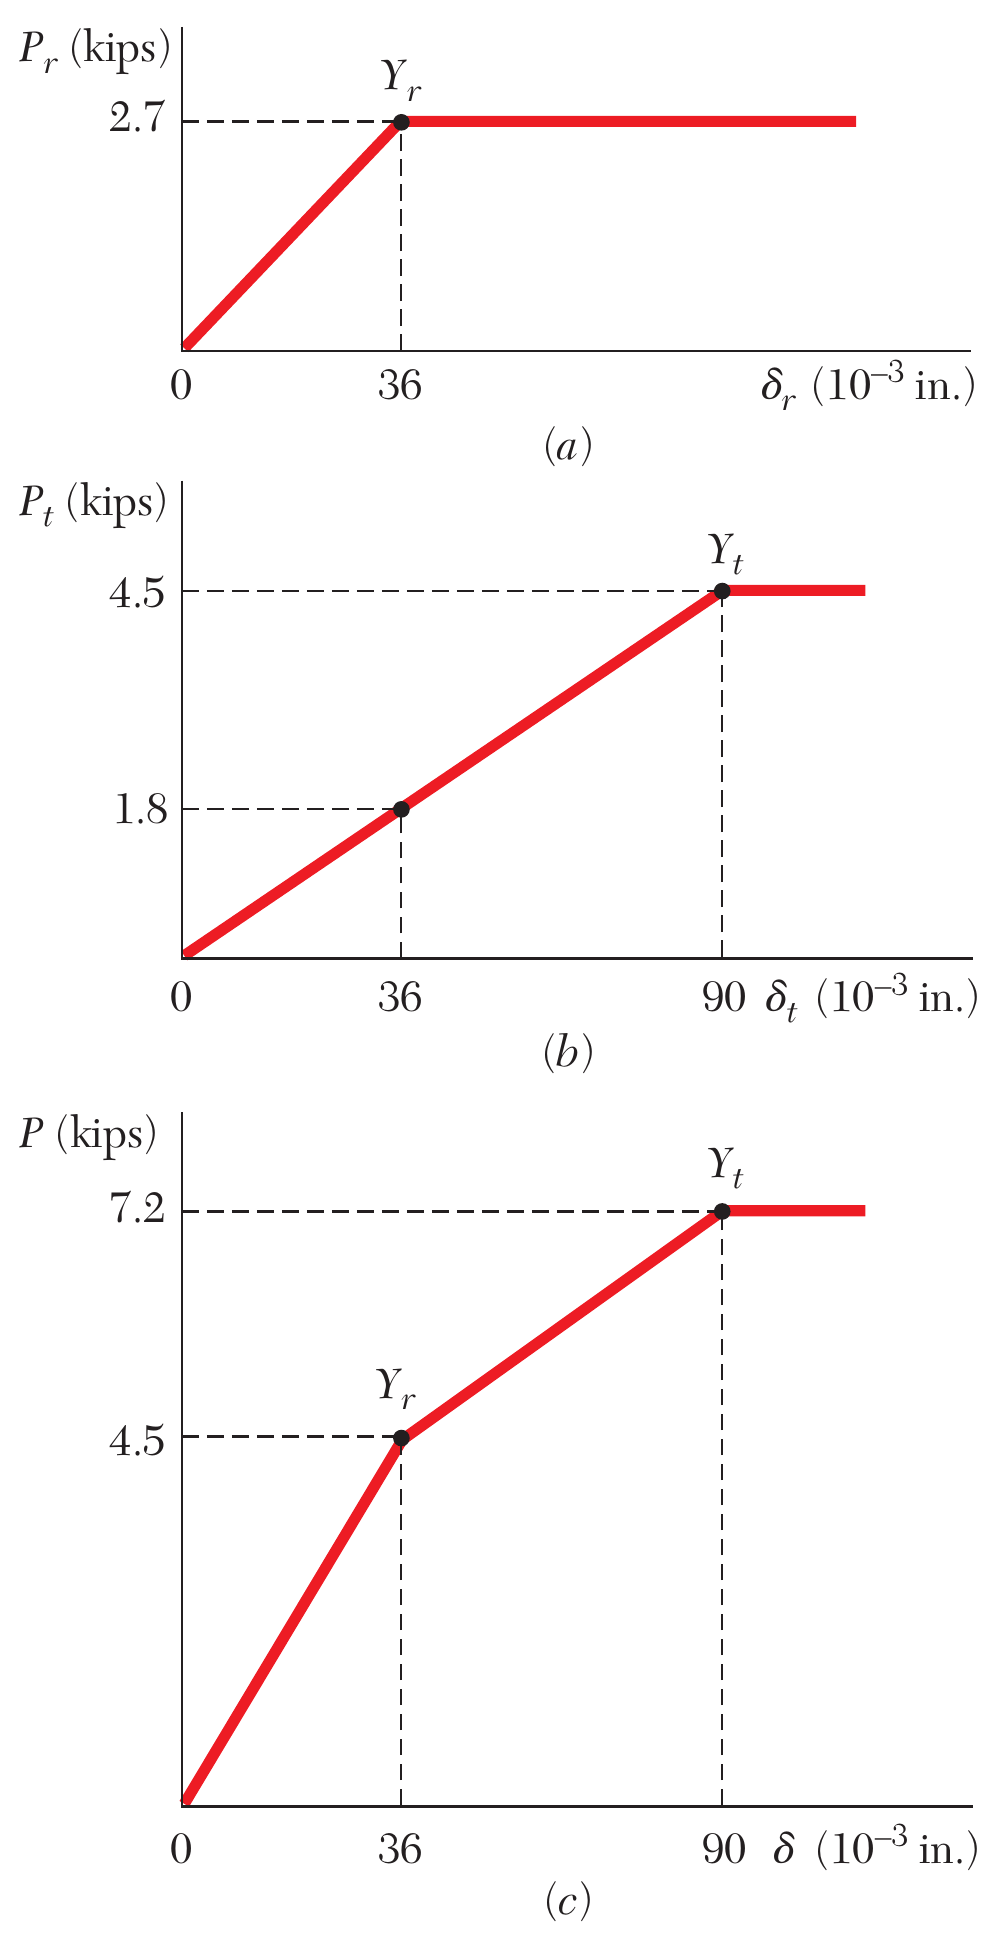
\includegraphics[width=\linewidth,height=7cm,keepaspectratio]{Chap_2/fig_2_63.png}
  \end{columns}
\end{frame}
% ===========
\begin{frame}[t]{Ví dụ 2.14, 2.15, 2.16 (tiếp)}
  \begin{columns}[T]
    \column{0.62\textwidth}
      \scriptsize
      b, c) Xác định độ giãn dài lớn nhất và biến dạng dư
      \begin{itemize}
        \setlength{\itemsep}{0.25em}
        \item Tại tải trọng $P = 25\,\mathrm{kN}$, thanh đã vào miền dẻo
              trong khi ống vẫn ở miền đàn hồi:
        \[
          P_r = (P_r)_Y = 12\,\mathrm{kN} \qquad
          P_t = P - P_r = (25 - 12)\,\mathrm{kN} = 13\,\mathrm{kN}
        \]
        \[
          \sigma_t = \frac{P_t}{A_t}
            = \frac{13\,\mathrm{kN}}{62\times10^{-6}\,\mathrm{m}^2}
            = 210\,\mathrm{MPa}
        \]
        \[
          \delta_t = \varepsilon_t L = \frac{\sigma_t}{E_t}L
            = \frac{210\times10^{6}}{105\times10^{9}}(750\,\mathrm{mm})
        \]
        \[
          \boxed{\delta_{\max} = \delta_t = 1{,}5\,\mathrm{mm}}
        \]
        \item Cụm thanh -- ống dỡ tải theo đường song song với $0Y_r$:
        \[
          m = \frac{19{,}2\,\mathrm{kN}}{0{,}89\,\mathrm{mm}}
            = 21{,}6\,\mathrm{kN/mm} = \text{độ dốc}
        \]
        \[
          \delta' = -\frac{P_{\max}}{m}
            = -\frac{25\,\mathrm{kN}}{21{,}6\,\mathrm{kN/mm}} = -1{,}16\,\mathrm{mm}
        \]
        \[
          \delta_p = \delta_{\max} + \delta' = (1{,}5 - 1{,}16)\,\mathrm{mm}
          \qquad \boxed{\delta_p = 0{,}34\,\mathrm{mm}}
        \]
      \end{itemize}
    \column{0.36\textwidth}
      \centering
      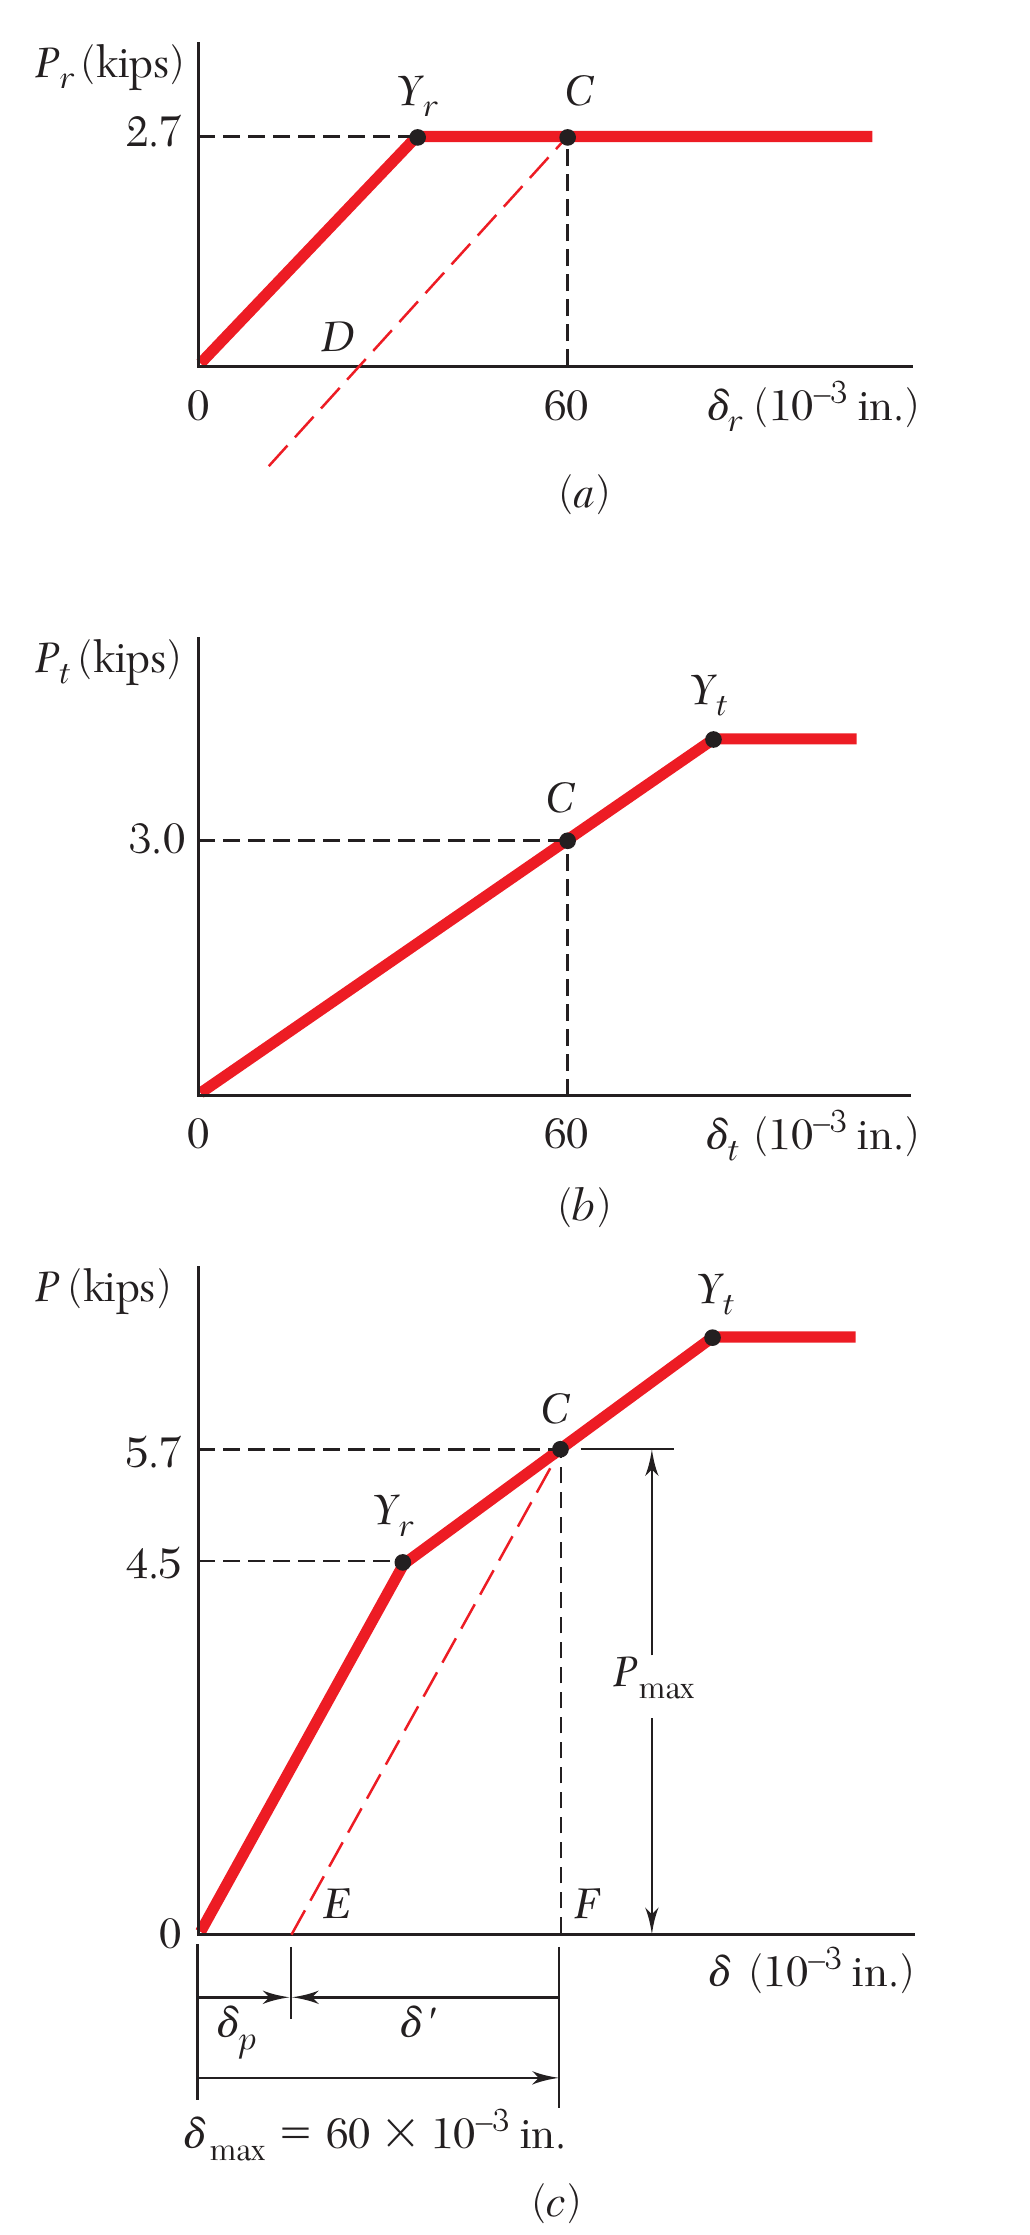
\includegraphics[width=\linewidth,height=7cm,keepaspectratio]{Chap_2/fig_2_64.png}
  \end{columns}
\end{frame}
% ===========
\begin{frame}[t]{Ví dụ 2.14, 2.15, 2.16 (tiếp)}
  \begin{columns}[T]
    \column{0.62\textwidth}
      \footnotesize
      d) Tính ứng suất dư trong thanh và ống.

      \vspace{0.3em}
      Tính ứng suất ngược trong thanh và ống do dỡ tải gây ra rồi cộng
      với ứng suất lớn nhất:
      \[
        \varepsilon' = \frac{\delta'}{L}
          = \frac{-1{,}16\,\mathrm{mm}}{750\,\mathrm{mm}}
          = -1{,}55\times10^{-3}\,\mathrm{mm/mm}
      \]
      \[
        \sigma'_r = \varepsilon'E_r = (-1{,}55\times10^{-3})(210\,\mathrm{GPa})
          = -325{,}5\,\mathrm{MPa}
      \]
      \[
        \sigma'_t = \varepsilon'E_t = (-1{,}55\times10^{-3})(105\,\mathrm{GPa})
          = -162{,}75\,\mathrm{MPa}
      \]
      \[
        \sigma_{\mathrm{dư},r} = \sigma_r + \sigma'_r
          = (250 - 325{,}5)\,\mathrm{MPa} = -75{,}5\,\mathrm{MPa}
      \]
      \[
        \sigma_{\mathrm{dư},t} = \sigma_t + \sigma'_t
          = (210 - 162{,}75)\,\mathrm{MPa} = 47{,}25\,\mathrm{MPa}
      \]
    \column{0.36\textwidth}
      \centering
      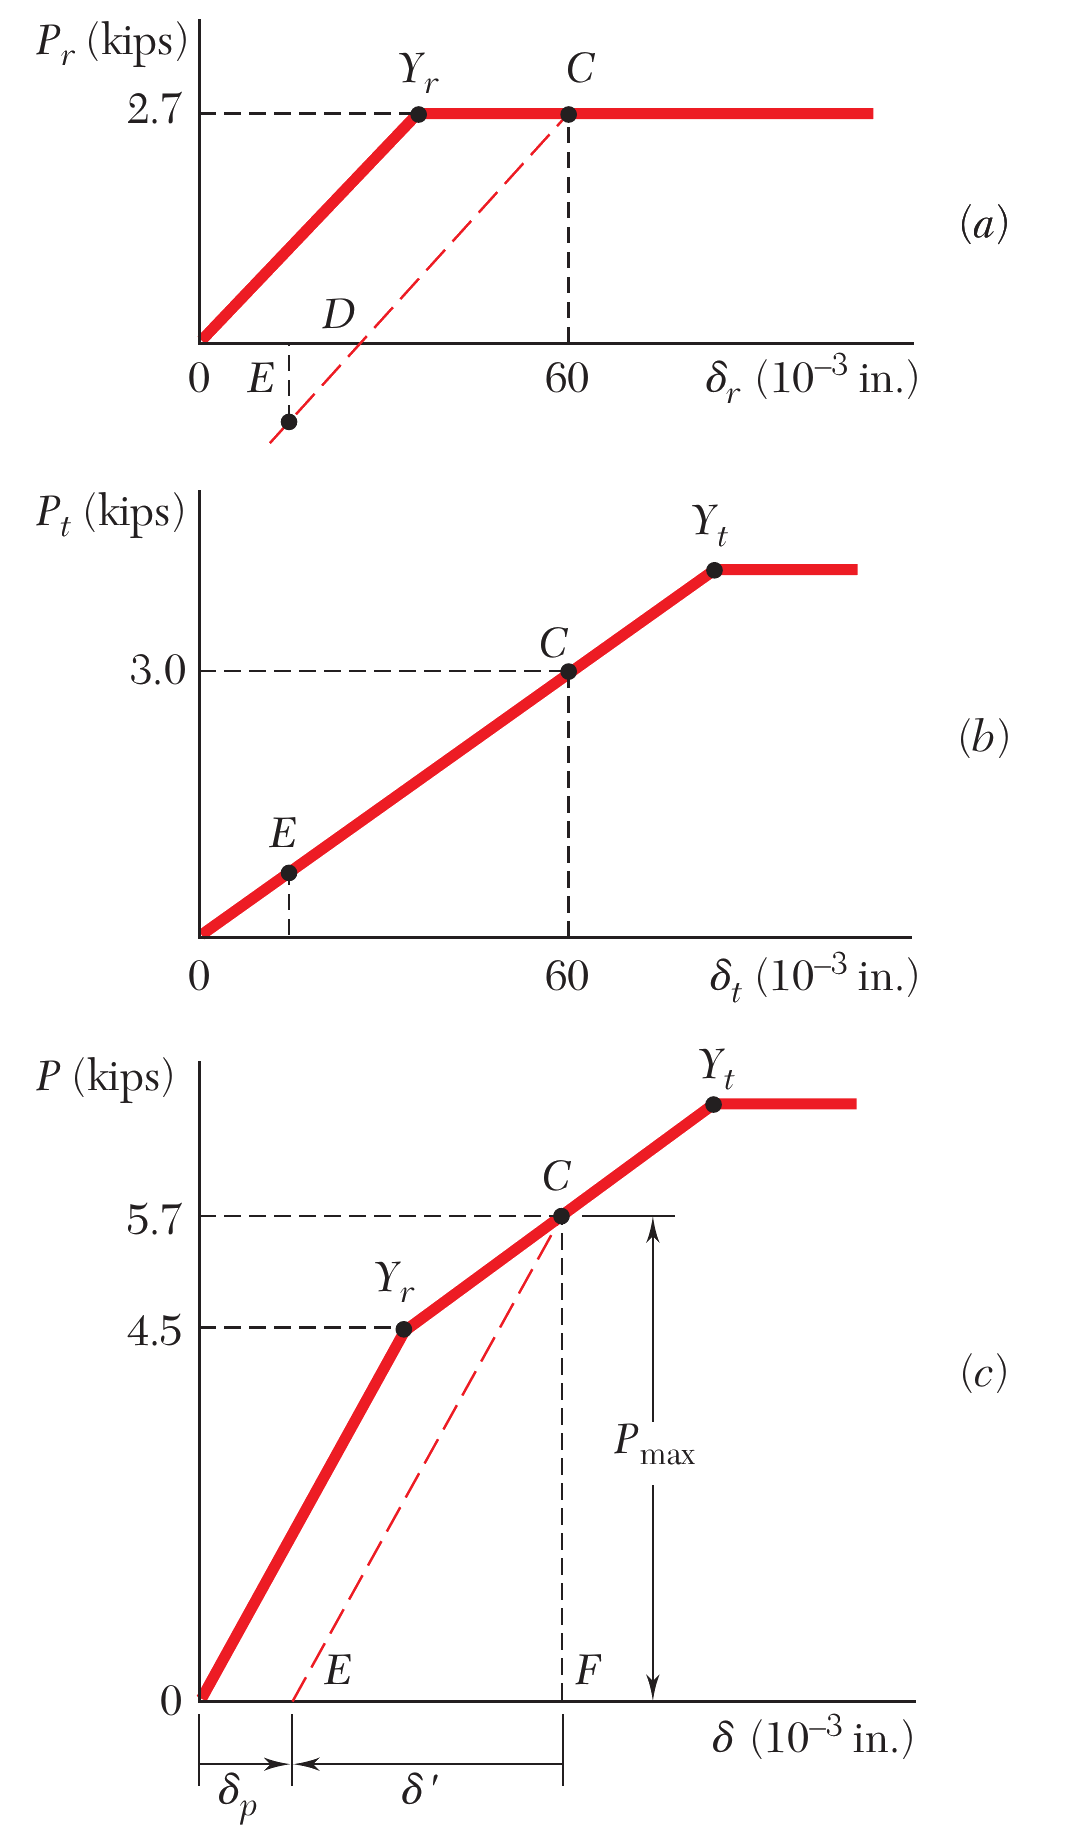
\includegraphics[width=\linewidth,height=6.5cm,keepaspectratio]{Chap_2/fig_2_66.png}
  \end{columns}
\end{frame}

\end{document}
